\documentclass[a4paper,twoside,11pt]{report}

\usepackage[english]{babel}
\usepackage{natbib}
\usepackage[left=2.5cm,right=2.5cm,top=3cm,bottom=3cm]{geometry}
\usepackage[hidelinks]{hyperref}
\usepackage{enumerate}
\usepackage{threeparttable}
\usepackage{mathtools}
\usepackage{graphicx}
\usepackage{epstopdf}
\epstopdfDeclareGraphicsRule
  {.tif}{png}{.png}{convert tif:\SourceFile.\SourceExt png:\OutputFile}
\AppendGraphicsExtensions{.tif}

\usepackage{xargs}
\usepackage[pdftex,dvipsnames]{xcolor}
\usepackage[colorinlistoftodos,prependcaption,textsize=tiny]{todonotes}
\newcommandx{\unsure}[2][1=]{\todo[linecolor=red,backgroundcolor=red!25,bordercolor=red,#1]{#2}}
\newcommandx{\change}[2][1=]{\todo[linecolor=blue,backgroundcolor=blue!25,bordercolor=blue,#1]{#2}}
\newcommandx{\info}[2][1=]{\todo[linecolor=OliveGreen,backgroundcolor=OliveGreen!25,bordercolor=OliveGreen,#1]{#2}}
\newcommandx{\improvement}[2][1=]{\todo[linecolor=Plum,backgroundcolor=Plum!25,bordercolor=Plum,#1]{#2}}
\newcommandx{\thiswillnotshow}[2][1=]{\todo[disable,#1]{#2}}

%set the number of sectioning levels that get number and appear in the contents
\setcounter{secnumdepth}{2}
\setcounter{tocdepth}{3}

\usepackage{graphicx}
\usepackage{verbatim}
\usepackage{latexsym}
\usepackage{mathchars}
\usepackage{setspace}
\usepackage[utf8]{inputenc}

\setlength{\parskip}{\medskipamount}  % a little space before a \par
\setlength{\parindent}{0pt}	      % don't indent first lines of paragraphs
%UHEAD.STY  If this is included after \documentstyle{report}, it adds
% an underlined heading style to the LaTeX report style.
% \pagestyle{uheadings} will put underlined headings at the top
% of each page. The right page headings are the Chapter titles and
% the left page titles are supplied by \def\lefthead{text}.

% Ted Shapin, Dec. 17, 1986

\makeatletter
\def\chapapp2{Chapter}

\def\appendix{\par
 \setcounter{chapter}{0}
 \setcounter{section}{0}
 \def\chapapp2{Appendix}
 \def\@chapapp{Appendix}
 \def\thechapter{\Alph{chapter}}}

\def\ps@uheadings{\let\@mkboth\markboth
% modifications
\def\@oddhead{\protect\underline{\protect\makebox[\textwidth][l]
		{\sl\rightmark\hfill\rm\thepage}}}
\def\@oddfoot{}
\def\@evenfoot{}
\def\@evenhead{\protect\underline{\protect\makebox[\textwidth][l]
		{\rm\thepage\hfill\sl\leftmark}}}
% end of modifications
\def\chaptermark##1{\markboth {\ifnum \c@secnumdepth >\m@ne
 \chapapp2\ \thechapter. \ \fi ##1}{}}%
\def\sectionmark##1{\markright {\ifnum \c@secnumdepth >\z@
   \thesection. \ \fi ##1}}}
\makeatother
%%From: marcel@cs.caltech.edu (Marcel van der Goot)
%%Newsgroups: comp.text.tex
%%Subject: illegal modification of boxit.sty
%%Date: 28 Feb 92 01:10:02 GMT
%%Organization: California Institute of Technology (CS dept)
%%Nntp-Posting-Host: andromeda.cs.caltech.edu
%%
%%
%%Quite some time ago I posted a file boxit.sty; maybe it made it
%%to some archives, although I don't recall submitting it. It defines
%%	\begin{boxit}
%%	...
%%	\end{boxit}
%%to draw a box around `...', where the `...' can contain other
%%environments (e.g., a verbatim environment). Unfortunately, it had
%%a problem: it did not work if you used it in paragraph mode, i.e., it
%%only worked if there was an empty line in front of \begin{boxit}.
%%Luckily, that is easily corrected.
%%
%%HOWEVER, apparently someone noticed the problem, tried to correct it,
%%and then distributed this modified version. That would be fine with me,
%%except that:
%%1. There was no note in the file about this modification, it only has my
%%   name in it.
%%2. The modification is wrong: now it only works if there is *no* empty
%%   line in front of \begin{boxit}. In my opinion this bug is worse than
%%   the original one.
%%
%%In particular, the author of this modification tried to force an empty
%%line by inserting a `\\' in the definition of \Beginboxit. If you have
%%a version of boxit.sty with a `\\', please delete it. If you have my
%%old version of boxit.sty, please also delete it. Below is an improved
%%version.
%%
%%Thanks to Joe Armstrong for drawing my attention to the bug and to the
%%illegal version.
%%
%%                                          Marcel van der Goot
%% .---------------------------------------------------------------
%% | Blauw de viooltjes,                    marcel@cs.caltech.edu
%% |    Rood zijn de rozen;
%% | Een rijm kan gezet
%% |    Met plaksel en dozen.
%% |


% boxit.sty
% version: 27 Feb 1992
%
% Defines a boxit environment, which draws lines around its contents.
% Usage:
%   \begin{boxit}
%	... (text you want to be boxed, can contain other environments)
%   \end{boxit}
%
% The width of the box is the width of the contents.
% The boxit* environment behaves the same, except that the box will be
% at least as wide as a normal paragraph.
%
% The reason for writing it this way (rather than with the \boxit#1 macro
% from the TeXbook), is that now you can box verbatim text, as in
%   \begin{boxit}
%   \begin{verbatim}
%   this better come out in boxed verbatim mode ...
%   \end{verbatim}
%   \end{boxit}
%
%						Marcel van der Goot
%						marcel@cs.caltech.edu
%

\def\Beginboxit
   {\par
    \vbox\bgroup
	   \hrule
	   \hbox\bgroup
		  \vrule \kern1.2pt %
		  \vbox\bgroup\kern1.2pt
   }

\def\Endboxit{%
			      \kern1.2pt
		       \egroup
		  \kern1.2pt\vrule
		\egroup
	   \hrule
	 \egroup
   }	

\newenvironment{boxit}{\Beginboxit}{\Endboxit}
\newenvironment{boxit*}{\Beginboxit\hbox to\hsize{}}{\Endboxit}
\pagestyle{empty}

\setlength{\parskip}{2ex plus 0.5ex minus 0.2ex}
\setlength{\parindent}{0pt}

\makeatletter  %to avoid error messages generated by "\@". Makes Latex treat "@" like a letter

\linespread{1}
\def\submitdate#1{\gdef\@submitdate{#1}}
\def\director#1{\gdef\@director{#1}}
\def\directortwo#1{\gdef\@directortwo{#1}}

\def\maketitle{
  \begin{titlepage}{
  
\includegraphics[height=17mm]{Images/LogoUPC.eps}

    \vskip 0.5cm
    \textsc{Programa de Doctorat en Enginyeria Biom\`{e}dica\\
    		\vskip 0.1cm
           Departament d'Enginyeria de Sistemes,\\ 
           Autom\`{a}tica i Inform\`{a}tica Industrial\\
           \vskip 0.1cm
           Centre de Recerca en Enginyeria Biom\`{e}dica}

    \rm
    \vskip 4cm
    
  \textbf{\Large \textsc Tesis Doctoral por compendio de publicaciones}\\
  \vspace{0.5cm}
    \Large \bf \@title \par
  }
  \vskip 1cm
  \par
  {\Large \@author}\\
   \vskip 0.2cm
  \Large{\@submitdate}

  \vskip 3cm
  
	\Large{Directores:\\ }
    {\Large \@director}\\
    {\Large \@directortwo}\\
  \vfil
  \end{titlepage}
}

\def\titlepage{
  \newpage
  \centering
  \linespread{1}
  \normalsize
  \vbox to \vsize\bgroup\vbox to 9in\bgroup
}
\def\endtitlepage{
  \par
  \kern 0pt
  \egroup
  \vss
  \egroup
  \cleardoublepage
}

\def\abstract{
    \LARGE \textbf{Abstract}
  \small
  %\def\baselinestretch{1.5}
  \linespread{1.5}
  \normalsize
}
\def\endabstract{
  \par
}

\def\resumen{
    \LARGE \textbf{Resumen}
  \small
  %\def\baselinestretch{1.5}
  \linespread{1.5}
  \normalsize
}
\def\endabstract{
  \par
}

\newenvironment{acknowledgements}{
  \cleardoublepage
  \begin{center}{
    \large \bf Acknowledgements}
  \end{center}
  \small
  \linespread{1.5}
  \normalsize
}{\cleardoublepage}
\def\endacknowledgements{
  \par
}

\newenvironment{dedication}{
  \cleardoublepage
  \begin{center}{
    \large \bf Dedication}
  \end{center}
  \small
  \linespread{1.5}
  \normalsize
}{\cleardoublepage}
\def\enddedication{
  \par
}

\def\preface{
    \pagenumbering{roman}
    \pagestyle{plain}
    \doublespacing
}

\def\body{
    \cleardoublepage    
    \pagestyle{uheadings}
    \tableofcontents
    \pagestyle{plain}
    \cleardoublepage
    \pagestyle{uheadings}
    \phantomsection
    \addcontentsline{toc}{chapter}{\listtablename}
    \listoftables
    \pagestyle{plain}
    \cleardoublepage
    \pagestyle{uheadings}
    \phantomsection
    \addcontentsline{toc}{chapter}{\listfigurename}
    \listoffigures
    \pagestyle{plain}
    \cleardoublepage
    \pagestyle{uheadings}
    \pagenumbering{arabic}
    \doublespacing
}

\makeatother  %to avoid error messages generated by "\@". Makes Latex treat "@" like a letter

\newcommand{\ipc}{{\sf ipc}}

\newcommand{\Prob}{\bbbp}
\newcommand{\Real}{\bbbr}
\newcommand{\real}{\Real}
\newcommand{\Int}{\bbbz}
\newcommand{\Nat}{\bbbn}

\newcommand{\NN}{{\sf I\kern-0.14emN}}   % Natural numbers
\newcommand{\ZZ}{{\sf Z\kern-0.45emZ}}   % Integers
\newcommand{\QQQ}{{\sf C\kern-0.48emQ}}   % Rational numbers
\newcommand{\RR}{{\sf I\kern-0.14emR}}   % Real numbers
\newcommand{\KK}{{\cal K}}
\newcommand{\OO}{{\cal O}}
\newcommand{\AAA}{{\bf A}}
\newcommand{\HH}{{\bf H}}
\newcommand{\II}{{\bf I}}
\newcommand{\LL}{{\bf L}}
\newcommand{\PP}{{\bf P}}
\newcommand{\PPprime}{{\bf P'}}
\newcommand{\QQ}{{\bf Q}}
\newcommand{\UU}{{\bf U}}
\newcommand{\UUprime}{{\bf U'}}
\newcommand{\zzero}{{\bf 0}}
\newcommand{\ppi}{\mbox{\boldmath $\pi$}}
\newcommand{\aalph}{\mbox{\boldmath $\alpha$}}
\newcommand{\bb}{{\bf b}}
\newcommand{\ee}{{\bf e}}
\newcommand{\mmu}{\mbox{\boldmath $\mu$}}
\newcommand{\vv}{{\bf v}}
\newcommand{\xx}{{\bf x}}
\newcommand{\yy}{{\bf y}}
\newcommand{\zz}{{\bf z}}
\newcommand{\oomeg}{\mbox{\boldmath $\omega$}}
\newcommand{\res}{{\bf res}}
\newcommand{\cchi}{{\mbox{\raisebox{.4ex}{$\chi$}}}}
%\newcommand{\cchi}{{\cal X}}
%\newcommand{\cchi}{\mbox{\Large $\chi$}}

% Logical operators and symbols
\newcommand{\imply}{\Rightarrow}
\newcommand{\bimply}{\Leftrightarrow}
\newcommand{\union}{\cup}
\newcommand{\intersect}{\cap}
\newcommand{\boolor}{\vee}
\newcommand{\booland}{\wedge}
\newcommand{\boolimply}{\imply}
\newcommand{\boolbimply}{\bimply}
\newcommand{\boolnot}{\neg}
\newcommand{\boolsat}{\!\models}
\newcommand{\boolnsat}{\!\not\models}


\newcommand{\op}[1]{\mathrm{#1}}
\newcommand{\s}[1]{\ensuremath{\mathcal #1}}

% Properly styled differentiation and integration operators
\newcommand{\diff}[1]{\mathrm{\frac{d}{d\mathit{#1}}}}
\newcommand{\diffII}[1]{\mathrm{\frac{d^2}{d\mathit{#1}^2}}}
\newcommand{\intg}[4]{\int_{#3}^{#4} #1 \, \mathrm{d}#2}
\newcommand{\intgd}[4]{\int\!\!\!\!\int_{#4} #1 \, \mathrm{d}#2 \, \mathrm{d}#3}

% Large () brackets on different lines of an eqnarray environment
\newcommand{\Leftbrace}[1]{\left(\raisebox{0mm}[#1][#1]{}\right.}
\newcommand{\Rightbrace}[1]{\left.\raisebox{0mm}[#1][#1]{}\right)}

% Funky symobols for footnotes
\newcommand{\symbolfootnote}{\renewcommand{\thefootnote}{\fnsymbol{footnote}}}
% now add \symbolfootnote to the beginning of the document...

\newcommand{\normallinespacing}{\renewcommand{\baselinestretch}{1.5} \normalsize}
\newcommand{\mediumlinespacing}{\renewcommand{\baselinestretch}{1.2} \normalsize}
\newcommand{\narrowlinespacing}{\renewcommand{\baselinestretch}{1.0} \normalsize}
\newcommand{\bump}{\noalign{\vspace*{\doublerulesep}}}
\newcommand{\cell}{\multicolumn{1}{}{}}
\newcommand{\spann}{\mbox{span}}
\newcommand{\diagg}{\mbox{diag}}
\newcommand{\modd}{\mbox{mod}}
\newcommand{\minn}{\mbox{min}}
\newcommand{\andd}{\mbox{and}}
\newcommand{\forr}{\mbox{for}}
\newcommand{\EE}{\mbox{E}}

\newcommand{\deff}{\stackrel{\mathrm{def}}{=}}
\newcommand{\syncc}{~\stackrel{\textstyle \rhd\kern-0.57em\lhd}{\scriptstyle L}~}

\def\coop{\mbox{\large $\rhd\!\!\!\lhd$}}
\newcommand{\sync}[1]{\raisebox{-1.0ex}{$\;\stackrel{\coop}{\scriptscriptstyle
#1}\,$}}

\newtheorem{definition}{Definition}[chapter]
\newtheorem{theorem}{Theorem}[chapter]

\newcommand{\Figref}[1]{Figure~\ref{#1}}
\newcommand{\fig}[3]{
 \begin{figure}[!ht]
 \begin{center}
 \scalebox{#3}{\includegraphics{figs/#1.ps}}
 \vspace{-0.1in}
 \caption[ ]{\label{#1} #2}
 \end{center}
 \end{figure}
}

\newcommand{\figtwo}[8]{
 \begin{figure}
 \parbox[b]{#4 \textwidth}{
 \begin{center}
 \scalebox{#3}{\includegraphics{figs/#1.ps}}
 \vspace{-0.1in}
 \caption{\label{#1}#2}
 \end{center}
 }
 \hfill
 \parbox[b]{#8 \textwidth}{
 \begin{center}
 \scalebox{#7}{\includegraphics{figs/#5.ps}}
 \vspace{-0.1in}
 \caption{\label{#5}#6}
 \end{center}
 }
 \end{figure}
}

\begin{document}

\title{\LARGE {\bf Muscular pattern based on multichanel surface EMG during voluntary contractions of the upper-limb}\\
 \vspace*{6mm}
}

\author{Mislav Jordanic}
\submitdate{September 2017}
\director{Miguel Angel Ma\~nanas Villanueva}
\directortwo{Mónica Rojas-Martínez}

\normallinespacing
\maketitle

\preface

\newpage
\phantomsection
\addcontentsline{toc}{chapter}{Abstract}

\begin{abstract}

Extraction of neuromuscular information is an important and extensively researched issue in biomedical engineering. Information on muscle control can be used in numerous human-machine interfaces and control applications, including rehabilitation engineering, e.g., prosthetics, exoskeletons and rehabilitation robots. 

Neuromuscular information can be extracted at the brain level, peripheral nerves, or muscles. Among these options, muscle interface is the only viable way of information extraction in everyday life. Although brain and nerve recordings are promising, they usually require invasive measurement and achieve relatively low extraction speed which prevents real time control. Even though in electromyographic (EMG) recordings information is not obtained directly from neural cells, it contains similar information as nerve recording. Information contained in action potential of the innervated muscle fibers (MUAP) is equivalent to the information contained in the action potential of corresponding motor neurons. Moreover, muscles contain multiple motor units that activate simultaneously so their electrical activity sums on the surface of the skin, resulting in a relatively high amplitude compared to the other bioelectrical signals. Therefore, due to the richness of neural information, noninvasiveness and high signal-to-noise ratio, the surface EMG is extensively used for man–machine interfacing, especially in commercial/clinical upper-limb prosthetic control.

Motivation and merit of this thesis lies in the fact that information associated with muscular pattern during exercises can be very useful in different applications such as monitoring patients’ control strategies during recovery, personalizing rehabilitation processes to increase their effectiveness or to provide information to be used for control of external devices (EMG based control of prosthesis or exoskeletons).

Within this doctorate a pattern recognition approach was used to assess neuromuscular information and to identify subjects' intended motion based on multichannel surface electromyographic recordings. Research was focused on control strategies of upper-limb, both in normal subjects and in patients with impaired mobility caused by incomplete spinal cord injury. Methods which are proposed can be used for the design and monitoring of rehabilitation therapies intended for patients with neuromuscular impairment, as well for the control of external devices like rehabilitation robots, exoskeletons, prostheses and even virtual games. However, that is in the domain of future applications and is not the scope of the thesis.

\end{abstract}
\newpage

\phantomsection
\addcontentsline{toc}{chapter}{Resumen}

\begin{resumen}

Texto aqui!

\end{resumen}
%\cleardoublepage

\addcontentsline{toc}{chapter}{Acknowledgements}

\begin{acknowledgements}

\narrowlinespacing
\begin{myquote}
\begin{flushright}
%Soyons reconnaissants aux personnes qui nous donnent du bonheur, elles sont les charmants jardiniers par qui nos âmes sont fleuries.\\
\textit{Let us be grateful to people who make us happy,\\they are the charming gardeners who make our souls blossom.} \\-- Marcel Proust
\end{flushright}
\end{myquote}
\normallinespacing

Writing this section is an act that demands more social responsibility than writing the rest of the thesis. The interesting fact is that most “readers” will pay great care only to this paragraphs and only rapidly turn the other 150 pages by a firm grip of the thumb and the index finger, a so called \emph{key grip}. (In a digital society most of us live in, the equivalent would be “by rapidly swirling the mouse wheel”.)

They are the people I met through live, whose friendship influenced me and my personality. To them I owe gratitude for who I am (or not!). They all mean a lot to me, whether we are no longer in contact, we are in contact, or we exchange faithfully four e-mails per year. They all deserve to be mentioned by name, but that would require appendix D. I can, however, mention them in a string of characters, in no particular order: T, A, Š, S, M, M, N, I, M, M, M, K, K, M, D, Dj, B, M, J, E, 1., 2., P, I, S, T, A, K, A, T, L, S, Dr. M, K, Z, V, E, A, I, R, N, D, C, V, L.

These readers are also my family, to whom I always stand in debt. To my wonderful parents, a dangerous collision of empathy and feelings from one side and logic and stubbornness from the other, who always provided me with more than I needed and guided me with their wisdom through the important choices in life, which I would only occasionally choose. This required patience! Here I also have to thank Mirta, my sister, with whom I grew up, who always tolerated my misbehavior, and with whom I share precious memories from the early days of her life. 

I also need to express my gratitude to Albert, the man with a green thumb, a daydreamer who accepted me in his home remotely and in good faith, and greatly facilitated my acclimatization to Barcelona. His ability to produce chaos is beyond anything I encountered with, but without him I would be lost. Luckily, I gained an ally when Pau joined me in the battle against this bohemian mess. A true companion through dust, tools, and spoiled food.

My Catalan friends who are not Catalan at all! Ivan and Zvonko with whom I shared so many \emph{glasses-of-water} all along the city, mountain experiences, long drives, swims, sweatings, and early morning yoga classes. I particularly enjoyed our discussions on physics, electromagnetism, and linear algebra. These discussions would always start with a disagreement on the particular question or phenomena, but very quickly they would bring us to the elementary mathematics, where they would shortly come to an end because of lack of knowledge and arguments. Number $\pi$, for example. Where is it coming from? It's in every important equation... why? Where is it coming from?!!

On the other hand, there are people who might find interesting what I wrote here and who might even go further and read other chapters. My colleagues from whom I learned so much. Miguel Angel, who showed me trust from the beginning and guided me through this research with his knowledge and experience, for which I am grateful. I admire his ability to look at the problem from a different perspective and come up with a solution where there isn't any. He also has a unique ability to postpone tasks. Mónica, who introduced me to the field, answered thousands of questions, and mentored me patiently through these years. Joan Francesc, always existing reliably in the background, giving support at the crucial moments. Hamid, a kind fellow with whom I spent much less time than I wanted to. The volume of his knowledge amazes me. I also have to thank to the rest of the group. To Carolina, Leidy, and Alejandro for sharing the burden and despair of doctoral study. And to Sergio for being the faithful companion on Friday meetings. BIOART group is a lovely working environment which I grew fond of.

Finally, I have to thank to my wonderful companion Kate for standing beside me and sharing her life with me, in the beginning over Skype, and towards the end in Carrer de Roger. For all the travels, adventures, ups, and downs -- everything with a smile and goofy silliness. I am grateful to have a soulmate with so high compatibility, and a true friend. Her life energy and joy inspire me and sometimes it can be difficult to keep up with her. And I hope it always will be...

That's it! The corny cliché part is over! Everybody has been thanked to. But for the end I would also like to thank to myself. Without help I wouldn't get far, but without daring I wouldn't have even started. Coming to Barcelona was a lifelong experience that changed and broaden my perspective on many things. As Hunter S. Thompson wrote: “Maybe it meant something. Maybe not, in the long run, but no explanation, no mix of words or music or memories can touch that sense of knowing that you were there and alive in that corner of time and the world. Whatever it meant.”

\end{acknowledgements}
%\clearpage

\narrowlinespacing

\vspace*{7cm}
\begin{flushright}
 \hspace{5cm} \emph{To my family. I am who they made me to be. \\For the good or the bad.}
\end{flushright}
\normallinespacing
%\clearpage

\narrowlinespacing

%\vspace*{7cm}
%\begin{flushright}
% \hspace{5cm} "Reserve your right to think, for even to think wrongly is better than not to think at all."\\
%\emph{Hypatia}

\vspace*{7cm}
\begin{myquote}
\begin{flushright}
\textit{Maybe it meant something. Maybe not, in the long run, but no explanation, no mix of words
or music or memories can touch that sense of knowing that you were there and alive in that
corner of time and the world. Whatever it meant.} \\Hunter S. Thompson
\end{flushright}
\end{myquote}



\normallinespacing

\body
%

\chapter{Introduction}

Performing a movement is a complicated process that involves many physiological entities working in high coherence. It involves bones, tendons, nerves, and many other working in perfect harmony. Even the simplest movements are rarely performed using just one muscle. Everything we do involves high muscular coordination and constant and precise regulation. While standing, muscles of legs and trunk are constantly simultaneously co-contracting, maintaining balance.  
Muscle is a body tissue capable of transforming chemical energy to force. There are several muscle types: smooth, building internal organs, cardiac, building the heart, and skeletal. Only skeletal muscles can be controlled voluntarily and are used in locomotion. They are usually connected to bones with tendons (collagen fibers), as shown in figure \ref{fig:muscle}.

The neurons controlling the movement are organized in hierarchical fashion \citep{Widmaier2014}. In the highest level of hierarchy, the movement is conceived. Here the complex plan of intention is made. Very little is known about the exact location of neurons responsible for this task. Higher centers then transmit this command to the middle level structures, where the task is elaborated. Simultaneously, this middle level neurons receive the information from the receptors in muscles, skin, tendons, and join, but also from the visual system. Planning of the movement that is about to be performed is performed with respect to the space this movement will occupy, and detailed control signals for each muscle involved in the movement are generated. Centers involved in this tasks are located in cerebral cortex, cerebellum, subcortical nuclei, and brainstem. The information is then transmitted to the lowest level of the motor hierarchy: spinal cord and brainstem. Here the information is transmitted over motor neurons to the muscles. The selection of motor neurons involved in the task and timing is performed at this level. Organization and locations of the neural system for motor control can be seen in figure \ref{fig:brain_centers}, whereas overall figure of motor control can be seen in figure \ref{fig:control-merletti}.
\begin{figure*}[t!]
    \centering
    \begin{subfigure}[t]{0.95\textwidth}
        \centering
        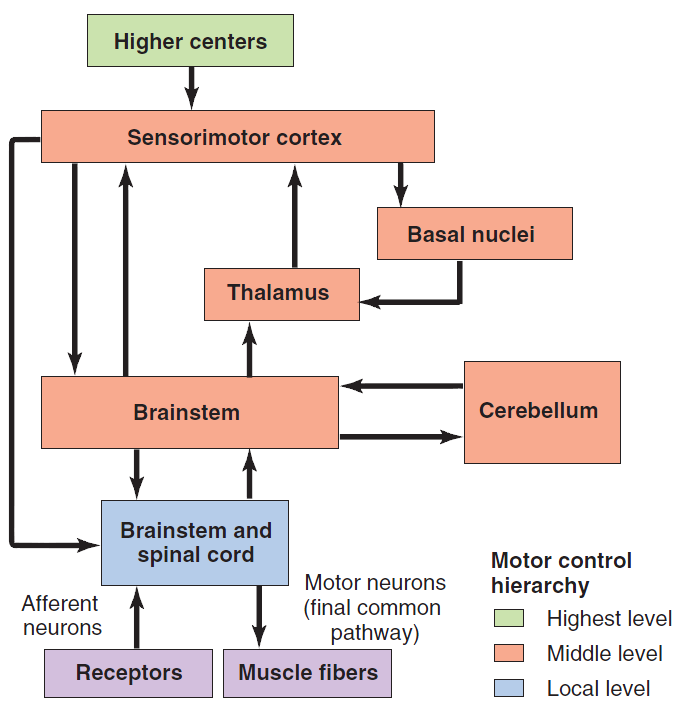
\includegraphics[height=3in]{Images/introduction/control.png}
        \caption{}
    \end{subfigure}%
    
    \begin{subfigure}[t]{0.95\textwidth}
        \centering
        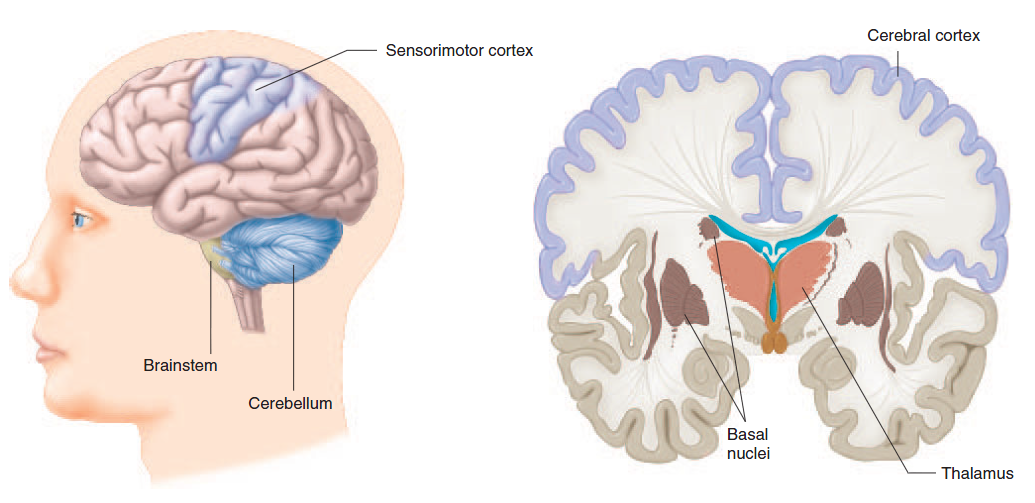
\includegraphics[height=3in]{Images/introduction/control2.png}
        \caption{}
    \end{subfigure}
    \caption{Figure describes \textbf{a)} hierarchical organization of neural system for motor control and \textbf{b)} side view and cross section of the brain showing motor control centers. Retrieved from \citep{Widmaier2014}}
\label{fig:brain_centers}
\end{figure*}

\begin{figure}[ht]
\centering
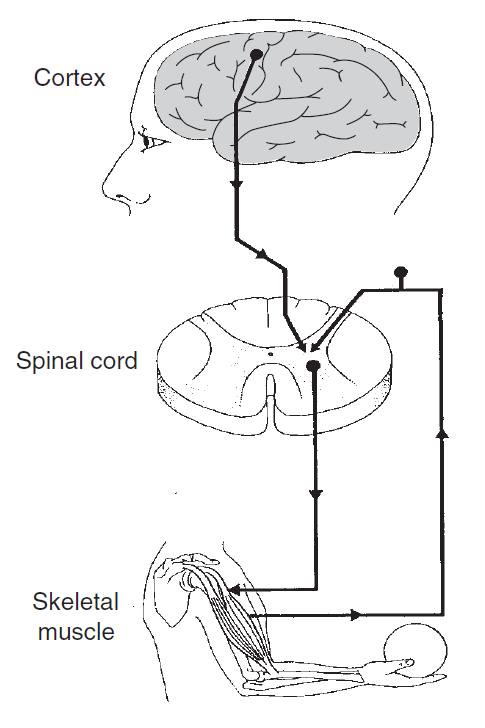
\includegraphics[width=0.45\textwidth]{Images/introduction/control-merletti2.png}
\caption{Figure represents a schematic representation of motor control mechanisms. Idea of a movement is conceived in the brain, and is getting to spinal cord by neural pathways. Motor neurons exiting spinal cord trigger muscle contraction. Simultaneously, sensory information is being transmitted to the higher controlling mechanisms. Retrieved from \citep{Merletti-book}}
\label{fig:control-merletti}
\end{figure}


\section{Muscle physiology}

Elementary building block of a muscle is muscle cell, or muscle fiber - \emph{myocyte}. They are ensheated by \emph{endomysium}, a connective tissue that contains nerves and capillaries. Myocytes are organized in bundles of 10 to 100 fibers, which are called \emph{fascicles}, and they are surrounded by sheath of connective tissue, \emph{perymisium}. Group of fascicles is finally grouped together and enveloped by \emph{epimysium}, forming a muscle. Muscle can be seen in figure \ref{fig:muscle}.
\begin{figure}[ht]
\centering
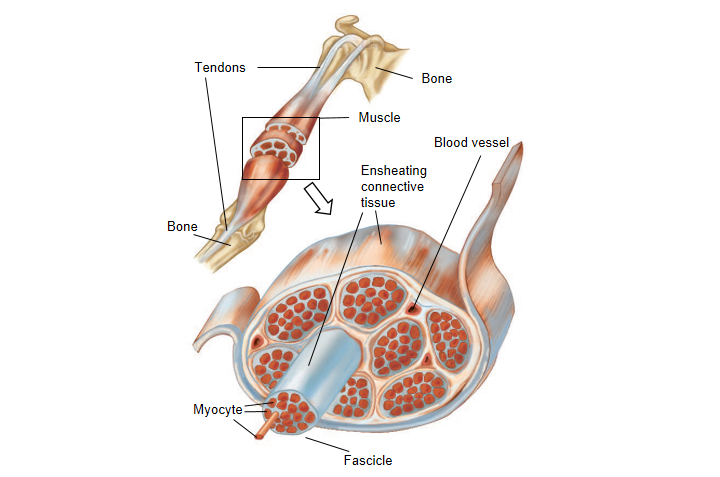
\includegraphics[width=0.9\textwidth]{Images/introduction/muscle2.png}
\caption{Organization of skeletal muscle with attachment to the bone. Retrieved from \citep{Widmaier2014}}
\label{fig:muscle}
\end{figure}

\emph{Sarcolema} is the cell membrane of myocyte, consisting of a lipid bilayer that contains intracelular liquid, \emph{myoplasma}. In the myoplasma, thin and thick filaments are serially connected, forming \emph{sarcomeres}, which are longitudinally connected in \emph{myofibrils} that extend through entire length of the myocyte. During shortening of muscle fibers, thin and thick filaments of sarcomeres are pulled together by cross-bridges between them. Total shortening of myofibril is summation of shortenings of sarcomeres of which it is composed.

Each motor neuron at the neuromuscular junction innervates several muscle fibers, forming the smallest functional unit called \emph{motor unit}. It was firstly defined by Liddell and Sherrington in 1925 \citep{Liddell1925, Sherrington1925} and is composed of motor neuron with axon and dendrites, and muscle fibers that axon innervates, as seen in the figure \ref{fig:motor units} \citep{Duchateau2011}. Since motor neuron with a single action potential usually evokes action potentials simultaneously in all belonging muscle fibers, by observing action potentials of the muscle fibers, information on activity of motor neurons in spinal cord or brain stem can be inferred \citep{Merletti-Farina-book}. Pool of motor neurons that innervates entire muscle generally ranges from ten to thousand, depending on the muscle \citep{Merletti-Farina-book}.
\begin{figure*}[t!]
    \centering
    \begin{subfigure}[t]{0.49\textwidth}
        \centering
        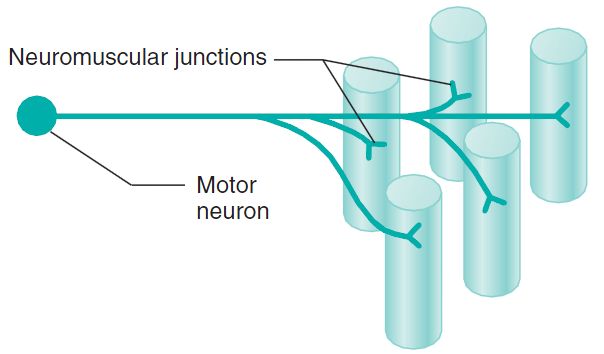
\includegraphics[height=1.7in]{Images/introduction/one_MU.png}
        \caption{}
    \end{subfigure}%
    ~ 
    \begin{subfigure}[t]{0.49\textwidth}
        \centering
        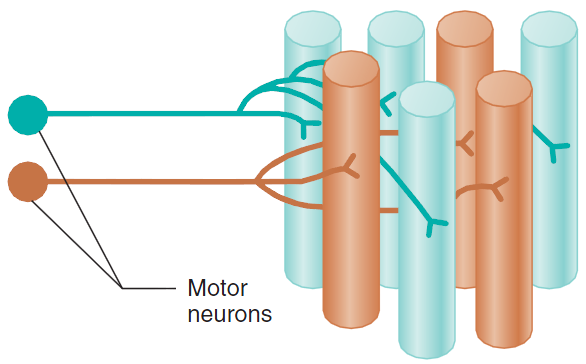
\includegraphics[height=1.7in]{Images/introduction/two_MU.png}
        \caption{}
    \end{subfigure}
    \caption{Figure shows \textbf{a)} a single motor unit with motoneuron and muscle fibers it innervates, and \textbf{b)} two motor units where it can be seen how muscle fibers of different motor units are intermingled. Retrieved from \citep{Widmaier2014}}
\label{fig:motor units}
\end{figure*}


By the characteristics of muscle fiber, there are three main types of muscle fibers:
\begin{description}
\item[Fast twitch, fatigable fibers (FF, or type IIb):] This fiber type have high levels of ATP (source of energy) for anaerobic energy supply, and are dominantly present in pale muscles. They are of glycolytic type and work well in ischemic or low oxygen conditions. Regarding contraction properties, they are characterized by fast twitch, large forces and high nerve conduction velocity, but they get fatigued faster than the other muscle fiber types. 

\item[Fast twitch, fatigue-resistant (FR, or type IIa):] These are oxidative glycolytic fibers, characterized by fast twitch and are resistant to fatigue. They have intermediate conduction velocity. 

\item[Slow twitch, very resistant to fatigue (S, or type I):] They are slow oxidative fibers and do not work well in low oxygen conditions. They generate small forces, have slow twitch and are characterized by lower nerve conduction velocity. This fiber type is very resilient to fatigue because of high oxidative metabolism and energy efficiency. They are present in high percentage in red muscles, such as soleus.
\end{description}

Muscle fibers innervated by the same motor neuron have similar histochemical and contractile characteristics, and can be said that motor unit is composed of the muscle fibers of the same type.

Force that muscle fibers generate depends on firing frequency of the action potentials (rate coding) innervating the neuromuscular junction, and the recruitment strategy by which the motor units are activated, i.e., the number of activated motor units. Firing frequency and the recruitment strategy depend on the speed and force of contraction. Muscle units with low threshold are activated firstly, resulting in low force and high endurance, i.e., resistance to fatigue. If greater force is required, muscle units with higher threshold that are prone to fatigue are activated \citep{Freund1975, Merletti-book}. This was firstly proposed by Henneman et al. in 1965 \citep{Henneman1965}, who state that order of recruitment of motor neurons is based on size principle, that is, neurons with smaller axons are recruited at lower effort levels and with increase in force, larger motoneurons are recruited. Therefore, S type muscle units, which have the smallest motoneurons are recruited first, followed by FR type units, and finally FF units. The recruitment strategy and resistance to fatigue can be seen in figure \ref{fig:fibers}. 

%\begin{figure}[ht]
%\centering
%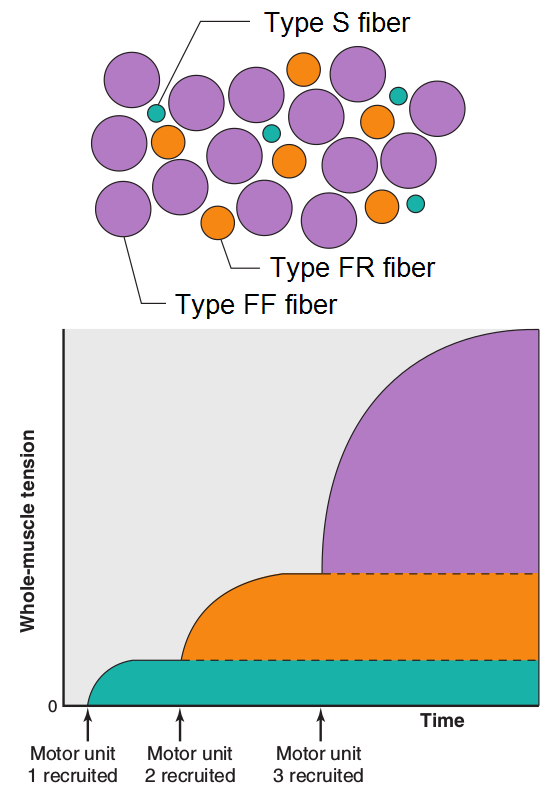
\includegraphics[width=0.5\textwidth]{Images/introduction/fiber_distribution.png}
%\caption{Figure illustrates \textbf{a)} diagram of different muscle fibers in muscle cross section, and \textbf{b)} muscle tension produced by recruitment of different types of muscle fiber. It can be noted that type S fibers are activated first and generate low force level, whereas type FF fibers are activated last and generate high forces . Adopted from Widmaier}
%\label{fig:fiber_distribution}
%\end{figure}
%
%\begin{figure}[ht]
%\centering
%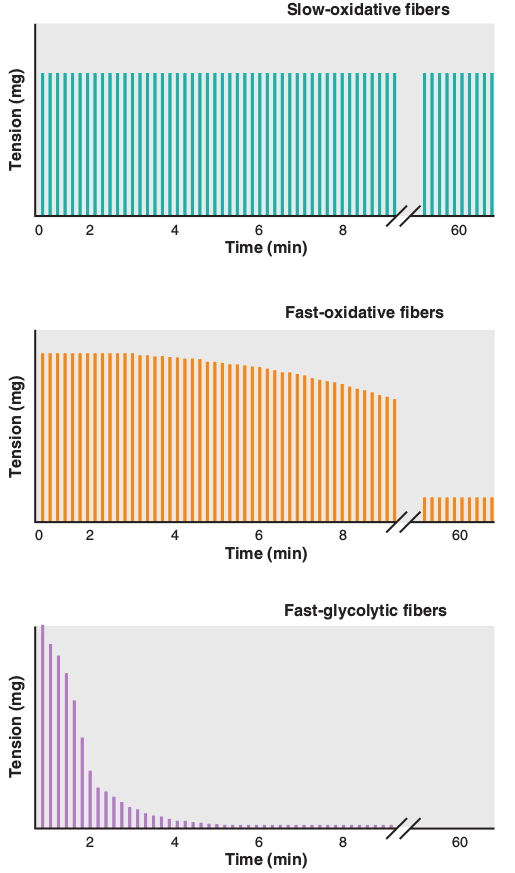
\includegraphics[width=0.5\textwidth]{Images/introduction/fiber_fatigue.png}
%\caption{Figure illustrates the time during which specific muscle fibers can remain tension. Adopted from Widmaier}
%\label{fig:fiber_fatigue}
%\end{figure}

\begin{figure*}[t!]
    \centering
    \begin{subfigure}[t]{0.45\textwidth}
        \centering
        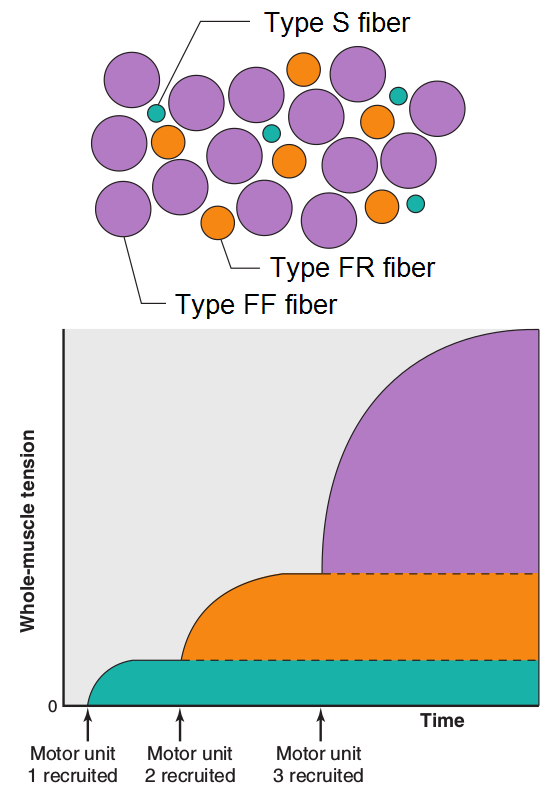
\includegraphics[height=4in]{Images/introduction/fiber_distribution.png}
        \caption{}
    \end{subfigure}%
    ~ 
    \begin{subfigure}[t]{0.45\textwidth}
        \centering
        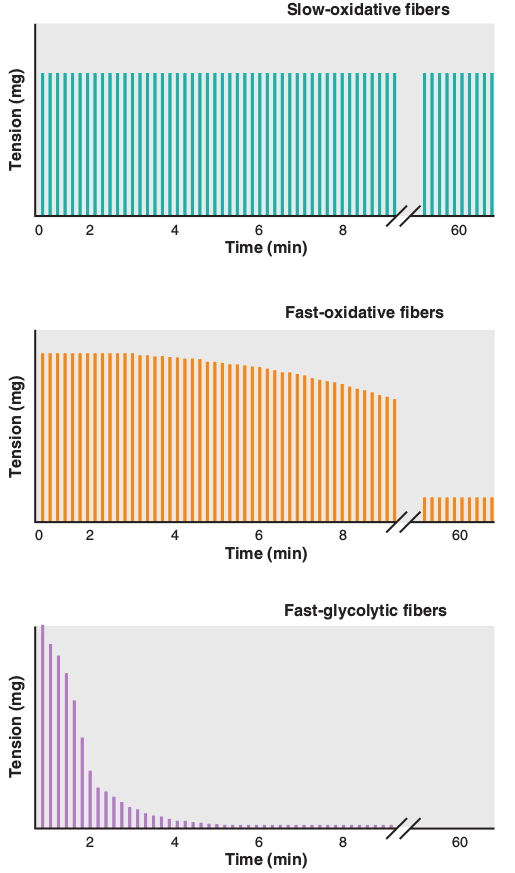
\includegraphics[height=4in]{Images/introduction/fiber_fatigue.png}
        \caption{}
    \end{subfigure}
    \caption{Figure describes characteristics of different types of muscle fibers. In \textbf{a)} is a diagram of different muscle fibers in muscle cross section (top), and muscle tension produced by recruitment of different types of muscle fiber (bottom), whereas in \textbf{b)} is the illustration of the time interval during which specific muscle fibers can remain tension. It can be noted that type S fibers are activated first, generate low force level, and are resistant to fatigue. On the other hand, type FF fibers are activated last, generate high forces, and develop fatigue fastest. Retrieved from \citep{Widmaier2014}}
\label{fig:fibers}
\end{figure*}


\section{Muscle contraction}

Skeletal muscles are activated voluntarily by electro-chemical impulses of motor neurons. The process is described in this chapter in summarized version. For more detailed description, the reader is pointed to medical literature (e.g. {Widmaier2014}).

During the stable state when there are no stimuli, i.e., in the resting state, the interior of the myocyte is at higher electrical potential that the exterior. This difference in potential is usually around 80 mV and it is caused by the higher concentration of positive ions, namely Na+, outside of the sarcolema \citep{Nazmi2016}, as shown in figure \ref{fig:depolarization}.

\begin{figure}[ht]
\centering
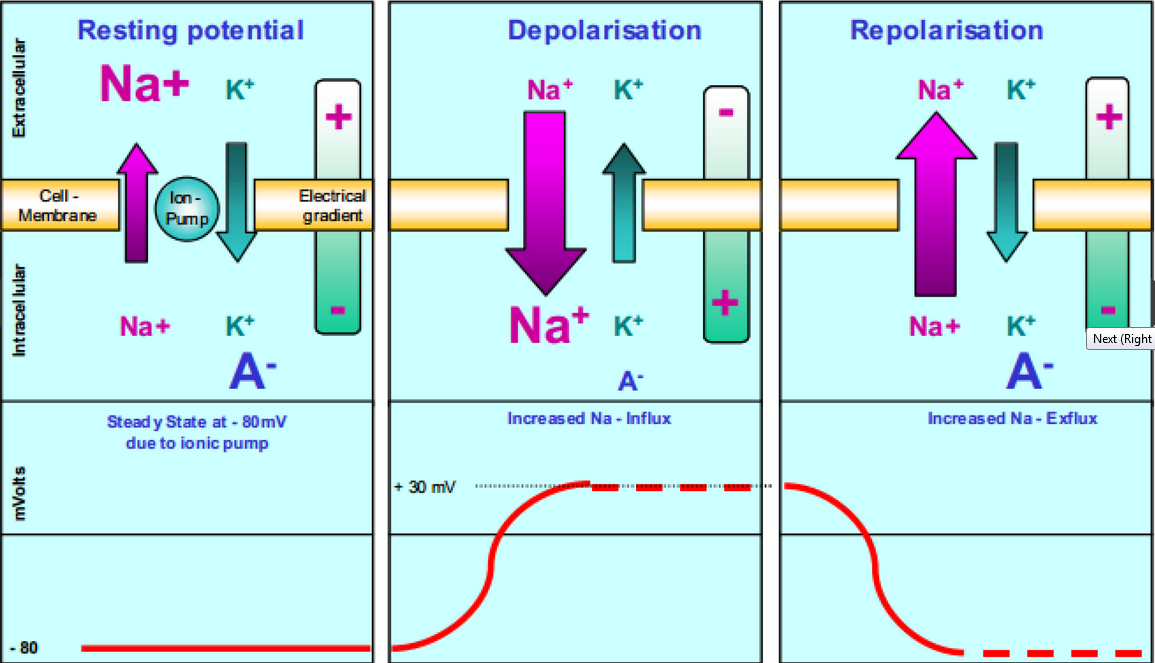
\includegraphics[width=0.95\textwidth]{Images/introduction/Depolarization.png}
\caption{Ilustration of depolarization/repolarization of the muscle fiber. Adopted from \citep{Nazmi2016}.}
\label{fig:depolarization}
\end{figure}

Motor neurons transfer nerve impulses that control the muscle from spinal cord to neuromuscular junction. At the nerve endings, action potentials induce the opening of calcium channels, which enables calcium from extracellular fluid to enter axon terminals and trigger the release of the neurotransmitter \emph{acetylcholine}. Acetylcholine is released to the narrow space between the axon and sarcolema of the myocyte, and causes sodium channels in sarcolema to open and allow the flow of Na+ and K+ ions in both directions. Na+ ions now flow into the myoplasma by diffusion due to higher concentration of Na+ ions outside of the membrane, but because of similar gradient, concentrations of the K+ ions don't change a lot. This process causes depolarization of sarcolema during which the outside potential of the muscle cell is at lower voltage than inside potential by around 30 mV. Depolarization is immediately followed by repolarization, a process during which the electrochemical balance and the resting potential of the cell are restored. It is achieved by flushing the Na+ ions outside of the sarcolema by the \emph{ion pump}. The process can be seen in figures \ref{fig:depolarization} and \ref{fig:action_potential_generation}.
  
\begin{figure}[ht]
\centering
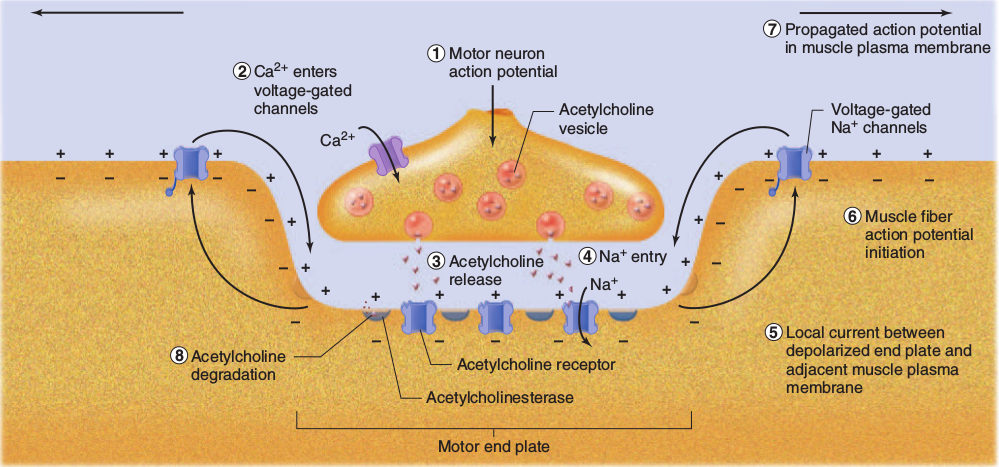
\includegraphics[width=0.95\textwidth]{Images/introduction/action_potential_generation.png}
\caption{Illustration of generation of action potential. Retrieved from \citep{Widmaier2014}.}
\label{fig:action_potential_generation}
\end{figure}
  
If the amount of acetylcoline is sufficient for the excitation, depolarization/repolarization wave, that is, action potential, propagates longitudinally from the neuromuscular junction towards the ends of the muscle fiber causing contraction \citep{Henneberg1999}. Speed of action potential propagation is called \emph{conduction velocity} and typically ranges around 4 m/s.

Detailed analysis of muscle physiology can be found elsewhere \citep{Squire1986, Widmaier2014}.



\section{Muscle fatigue} \label{sc:fatigue}

According to \citet{Widmaier2014}, muscle fatigue is a decline in muscle tension as a result of previous contractile activity. It is also characterized by decreased relaxation rate and lower shortening velocity of muscle fibers. Muscle fatigue is a continuous process that starts at the moment when muscle unit activates. If muscle keeps contracting long enough, eventually it will stop contracting because of electro-physiological inability to maintain the contraction. This moment is called the failure point \citep{DeLuca1984}. The failure point depends on many different factors physiological characteristics, but also on the number of muscle fibers and proportion of Type I/Type II muscle fibers. Muscles with higher proportion of Type I fibers do not fatigue easily and recover sooner than type II fibers. However, type II fibers are able to generate higher forces \citep{Kupa1995}.

Factors causing fatigue can be found in the muscle itself, which is \emph{peripheral fatigue}, but can also originate in central nervous system, in which case it is \emph{central fatigue}.

With respect to the source of impairment, the muscle fatigue can be:

\begin{description}

\item[Peripheral fatigue] \hfill \\
	Peripheral fatigue occurs in muscle itself, when because of electro-chemical imbalance muscle contraction is prevented. There are three main sources of peripheral fatigue:
	\begin{itemize}
		\item During sustained contraction, sarcolema of the muscle fibers become acid, and this accidifation lowers the muscle fiber conduction velocity \citep{DeLuca1984}.
		
		\item High concentration of K+ ions prevents generation of action potentials in muscle fiber \citep{Widmaier2014}. 
		
		\item Buildup of adenosine diphosphate, a byproduct of muscle contraction, slows the rate of cross-bridge cycling, affecting the relaxation, and reducing shortening velocity \citep{Widmaier2014}.
	\end{itemize}

\item[Central fatigue] \hfill \\
	Central fatigue occurs in central nervous system that controls the movement. It is manifested by synchronization of neural spike trains of different motor units. Probably by following the principle that by activating more muscle units simultaneously, total output force of the muscle is higher. 

\end{description}

Muscle fatigue changes characteristics of the myoelectric signal. Due to decrease of muscle fiber conduction velocity, caused by peripheral fatigue, but also due to synchronization of firing times caused by central fatigue, there is a shift of energy in frequency spectrum of myoelectric signal towards lower frequency, as shown in figure \ref{fig:fatigue} \citep{DeLuca1984}. Another indicator of muscle fatigue is increase of amplitude of surface electromyographic signal. This increase occurs due to two main reasons:
\begin{itemize}
\item Tissue between muscle fibers and recording electrodes positioned on the surface of the skin (e.g. fat layers, skin, etc.) have low-pass properties on the propagating electromagnetic wave. Since the power of the propagating wave shifts towards lower frequencies, amplitude of the recorded signal increase.

\item Due to synchronization of firing patterns cause by central fatigue, amplitude of recorded sEMG signal increases. 
\end{itemize} 

\begin{figure}[ht]
\centering
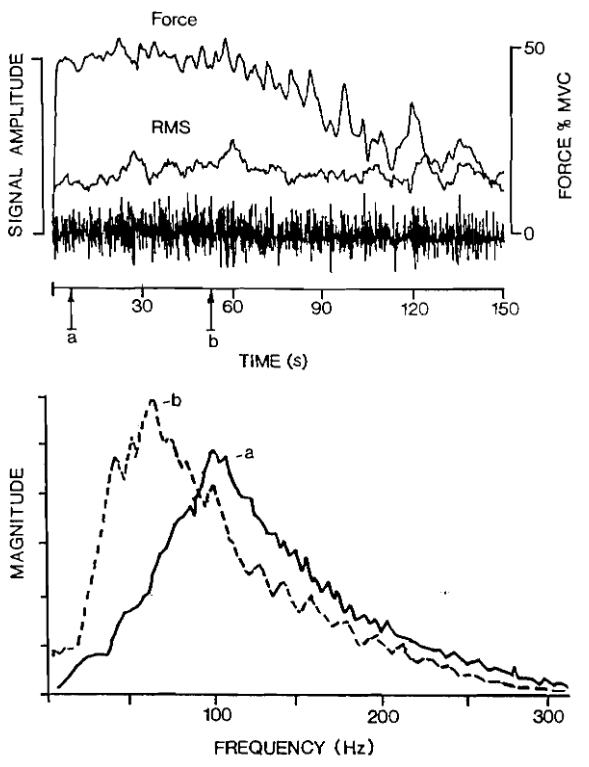
\includegraphics[width=0.45\textwidth]{Images/introduction/fatigue.png}
\caption{Illustration of force and EMG signal recorded during fatiguing exercise (top), and frequency spectra of corresponding EMG signal (bottom) recorded at the beginning of the exercise (a), and at time when force started decreasing (b). Retrieved from \citep{DeLuca1984}.}
\label{fig:fatigue}
\end{figure}

There are many studies exploiting this changes in sEMG signal to estimate and monitor muscle fatigue. Most of the approaches are based on monitoring frequency characteristics of the signal. One of the simplest measures is number of zero-crossings \citep{Hagg1981}, but it is very sensitive to noise. Mean and median frequencies are often used in literature \citep{Lindstrom1977, Merletti1997, Stulen1981}, but also more advanced time-frequency processing methods \citep{Knaflitz1999, Cifrek2000, Georgakis2003, Srhoj-Egekher2011a}.


\section{Surface electromyography}

Muscle unit action potentnial (MUAP) is the combination of action potentials generated by all muscle fibers belonging to that motor unit, whereas myoelectric signal is a superposition of electrical activity (propagating action potentials) produced by all muscle units. 

There are two main types of electromyographic measurements: 
\begin{description}
\item[Surface EMG (sEMG)] This is non-invasive type of EMG measurement where electrodes are positioned on the surface of the skin. Two types of electrodes are used: wet electrodes, which are used in combination with conductive gel that provide high signal quality, and dry electrodes, which can be applied directly on the skin. Although wet electrodes are mostly used, signal quality deteriorates during recording because of evaporation of the gel.

\item[Intramuscular EMG (iEMG)] This is invasive type of recording which implies insertion of needle or wire electrodes under the skin \citep{Marateb1999}. This type of recording is used for precise measurement of narrow volume, for example couple of muscle fibers. It has high SNR, but causes discomfort in subjects. It It is often used in clinical practice because it can detect abnormal functionality. For example, action potentials of spontaneously contracting single muscle fibers can be measured. These potentials are an important sign of deinnervation, but cannot be recorded using sEMG \citep{Merletti-book}.
\end{description}

Although iEMG signal usually has higher quality (in terms of signal-to-noise ratio), it was shown that both approaches provide a similar identification rate of upper-arm motor task \citep{Hargrove2007}. Since sEMG is non-invasive, it is usually preferred method in myocontrol. Moreover, although often narrow volume scope of iEMG can be beneficial, especially in clinical applications regarding activation of single muscle unit, it does not provide information on other parts of the muscle. For that reason, sEMG can be more appropriate because it simultaneously records action potentials of large muscle area. Depending on the application, that can also be a serious drawback because if there are several active muscles in small volume, myoelectric activity of both muscles will be recorded, i.e., there will be \emph{crosstalk} between muscles. 

Surface electromyographic signal is the sum of the electrical activity of the muscle fibers recorded on the surface of the skin. From statistical point of view, EMG signal can be considered as a non-stationary stochastic process whose probability density function is the Gaussian function. \citep{DeLuca1984, DeLuca1979}. Since muscle fibers are activated by the impulse train of the innervating motor neurons, i.e. neural drive to the muscle, sEMG is the convolution of motor neuron spike trains by the motor unit action potential recorded on the electrodes \citep{Farina2010, Farina2014}:

\begin{equation}
sEMG(t) = \sum_{i=1}^{M} \sum_{j=-\infty}^{+\infty} MUAP_i(t)\,\, \delta(t-t_{i,j})
\end{equation}

, where $M$ is the number of active motor units, $MUAP_i(t)$ is the action potential waveform of the $i^{th}$ motor unit recorded by the electrodes, and $t_{i,j}$ is the time of the discharge of the $i^{th}$ motor neuron. This model assumes there is no interference and that neuromuscular junction never fails, which is not the case. In the equation, $MUAP_i(t)$ is related to the electrophysiological state of the muscle fiber membranes and conduction properties of the tissue through which the potential propagates, whereas neural information is contained in motor neuron spike trains $\delta(t-t_{i,j})$ \citep{Farina2014b}. With respect to muscle fatigue explained in the previous section, peripheral fatigue affects $MUAP_i(t)$, whereas central fatigue have effect on $\delta(t-t_{i,j})$ term. It is important to notice that following this model, sEMG reflects all motor control information that is present in motor neuron. For that reason, it is more appropriate to extract motor control information carried by motor neurons using sEMG, than directly by invasive measurement of electrical potential of the motor neuron. The advantage of the sEMG is that multiple fibers are activated simultanously, generating bioelectrical signal with relatively high SNR, which can be measured on the surface of the skin. In this context, sEMG can be considered as the amplified neural signal, whereas muscle can be considered as a biological amplifier of nerve activity \citep{Farina2014}. Origin of sEMG signal can be seen in figure \ref{fig:EMG_origin}.
\begin{figure}[ht]
\centering
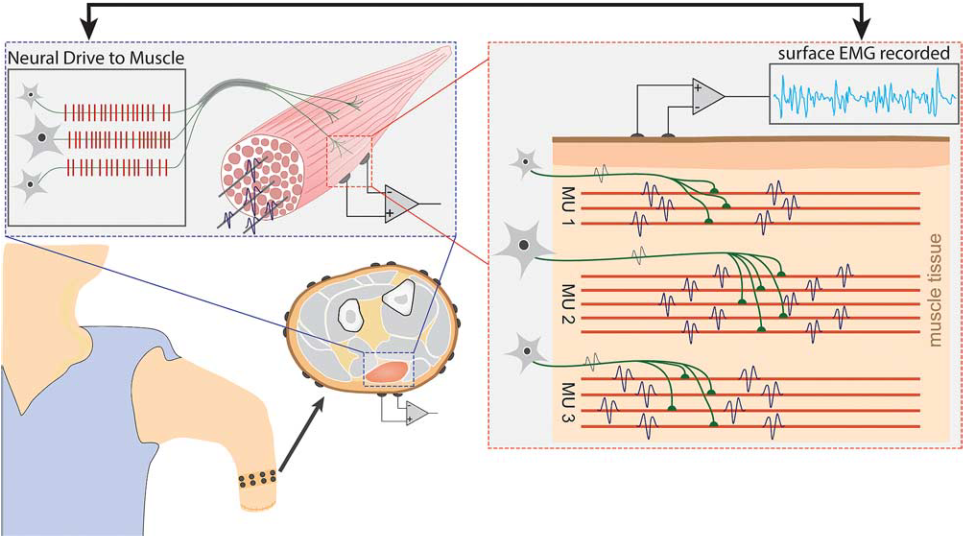
\includegraphics[width=0.75\textwidth]{Images/introduction/EMG_origin.png}
\caption{sEMG signal is a superposition of motor unit action potentials recorded on the electrodes convoluted by belonging motor neuron spike train. Retrieved from \citep{Farina2014}.}
\label{fig:EMG_origin}
\end{figure}

In frequency domain, motor unit action potential spike train provides both the neural and peripheral information:

\begin{equation}
P_{sEMG}(f) = \sum_{i=1}^{M} P_{ST_i}(f) \, \, \big\vert \Phi_{MUAP_i}(f) \big\vert^2
\end{equation}

,where $P_{sEMG}(f)$ is the power spectrum of sEMG signal, $\Phi_{MUAP_i}(f)$ is the Fourier transform of the $MUAP_i$, and $P_{ST_i}(f)$ is the power spectrum of the spike train that innervates it. It is assumed that spike trains are uncorrelated process \citep{Farina2014}.

In case of constant average discharge rate of spike trains (stationary process), spike train power spectrum can be calculated as:

\begin{equation}
P_{ST_i}(f) = DR_i \left[ 1- \big\vert Q_i(f)\big\vert^2 \right] + DR_i^2  \big\vert Q_i(f)\big\vert^2 \,  \sum_{n=-\infty}^{+\infty} \delta(f - n DR_i)
\end{equation}

, where $DR_i$ is the average discharge rate, and $Q_i(f)$ is the Fourier transform of the probability density function of the inter-spike interval variability. The first term in the equation is dominant and equal to $DR_i$ for frequencies greater than 10 - 20 Hz \citep{Lago1977, Farina2014}. Therefore, the power spectrum of the sEMG signal can be estimated as:

\begin{equation}
P_{sEMG}(f) \approx  \sum_{i=1}^{M} DR_i \, \big\vert Q_i(f)\big\vert^2
\end{equation}

Power of the EMG signal $P$ can be obtained in the frequency domain as:

\begin{equation}
P = \int_0^{+\infty} P_{sEMG}(f) \, df  \, \approx \, \sum_{i=1}^{M} DR_i \,E_i
\end{equation}

,where $E_i$ is the energy of $MUAP_i$. It can be noted that the power of sEMG is sum of energies of action potentials of motor units weighted by their discharge rate. When the force of contraction is increased, the power of EMG increases also because of the activation of additional motor units ($M$ increases) and because of the increase of the the average discharge rate of motor neuron action potentials ($DR_i$ increases). When the muscle is fatigued, the conduction velocity of muscle fibers decreases and the power spectrum of muscle fiber action potentials shifts towards lower frequencies, as explained in section \ref{sc:fatigue}. Due to this effect, energy of MUAPs recorded on the electrodes can increase, leading to increase of sEMG power ($E_i$ increases).

Given the fact that there is large variability between shape, and amplitude of MUAP with respect to electrode position and tissue conduction characteristics, the association between power of the sEMG and the neural drive can also have very high variability, depending on individual subject and muscle \citep{Farina2014}. 

Depending on number of electrodes used for the recording. the following classification exists: single-channel recording in monopolar mode, single channel recording in bipolar mode, recording using linear electrode array, and high-density EMG, as shown in figure \ref{fig:electrode_types}).
\begin{figure}[ht]
\centering
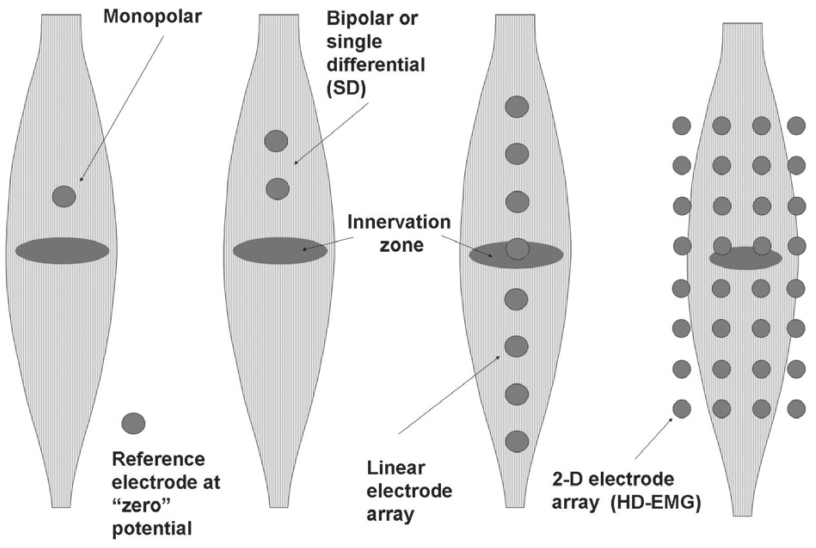
\includegraphics[width=0.65\textwidth]{Images/introduction/electrode_types.png}
\caption{Four types of recording surface EMG signal: monopolar, bipolar, linear electrode array, HD-EMG. Figure was modified from \citep{Merletti2010}.}
\label{fig:electrode_types}
\end{figure}

In single-channel monopolar recording, a single electrode is positioned over the muscle, whereas the reference electrode is positioned over the place that does not generate electrical activity. On the other hand, single-channel bipolar electrode configuration is most often used, in which signal is a difference of potential between two electrodes. These configuration is traditionally preferred because of the lower interference and higher signal-to-noise ration \citep{Merletti-book}. General recommendation is that the inter-electrode distance is around 20 cm \citep{Hermens1999}, but the optimal distance depends on many factors, as briefly explained in \citep{Hakonen2015}. For both monopolar and bipolar single channel recordings it is recommended that the electrodes are positioned between innervation zone and tendon. Exact recommendations can be found in the findings of the SENIAM project \citet{Hermens1999}.

Linear electrode array consists of multiple electrodes positioned at equal distance along the muscle line, folowing the direction of propagation of action potentials. Measurements recorded using this type of electrodes provide more information on the muscle. For example, it can be used for estimation of conduction velocity, as shown is figure \ref{fig:conduction_velocity} \citep{Merletti-book}.
\begin{figure}[ht]
\centering
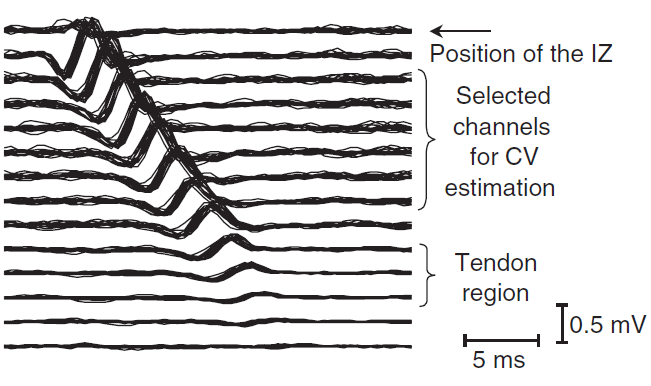
\includegraphics[width=0.60\textwidth]{Images/introduction/conduction_velocity.png}
\caption{Estimating conduction velocity using averaged MUAPs recorded using linear electrode array. Figure was retrieved from \citep{Merletti-book}.}
\label{fig:conduction_velocity}
\end{figure}

Technological advancement of EMG acquisition systems enables use of high-density electromyography (HD-EMG) \citep{Zwarts2004}. Using an array of closely spaced electrodes organized in a quadrature grid, multiple EMG channels are recorded over the wide area of the muscle. Electrodes used for HD-EMG recording can be seen in figure \ref{fig:electrode}. This type of recording is more reliable because it can record activations in different parts of the muscle and increase redundancy. HD-EMG is the only EMG recording approach that allows insights into spatial distribution of motor units in a muscle. By observing the amplitude or intensity of signals recorded in different channels, it is possible to analyze how different muscle regions activate depending on joint position \citep{Vieira2010}, contraction level \citep{Holtermann2005}, and duration of movement and fatigue \citep{Tucker2009, Staudenmann2014}. Moreover, Zwartz et al. pointed out that single channel EMG disregards important spatial aspects of MUAP propagation, which are essential for the force-generating capacity of the muscle, and, if not well addressed, can lead to incorrect conclusions \citep{Zwarts2003}. Moreover, since muscles do not activate homogeneously, single bipolar channel EMG has some serious drawbacks, which can be overcome by using 2D electrode arrays. 
\begin{figure}[ht]
\centering
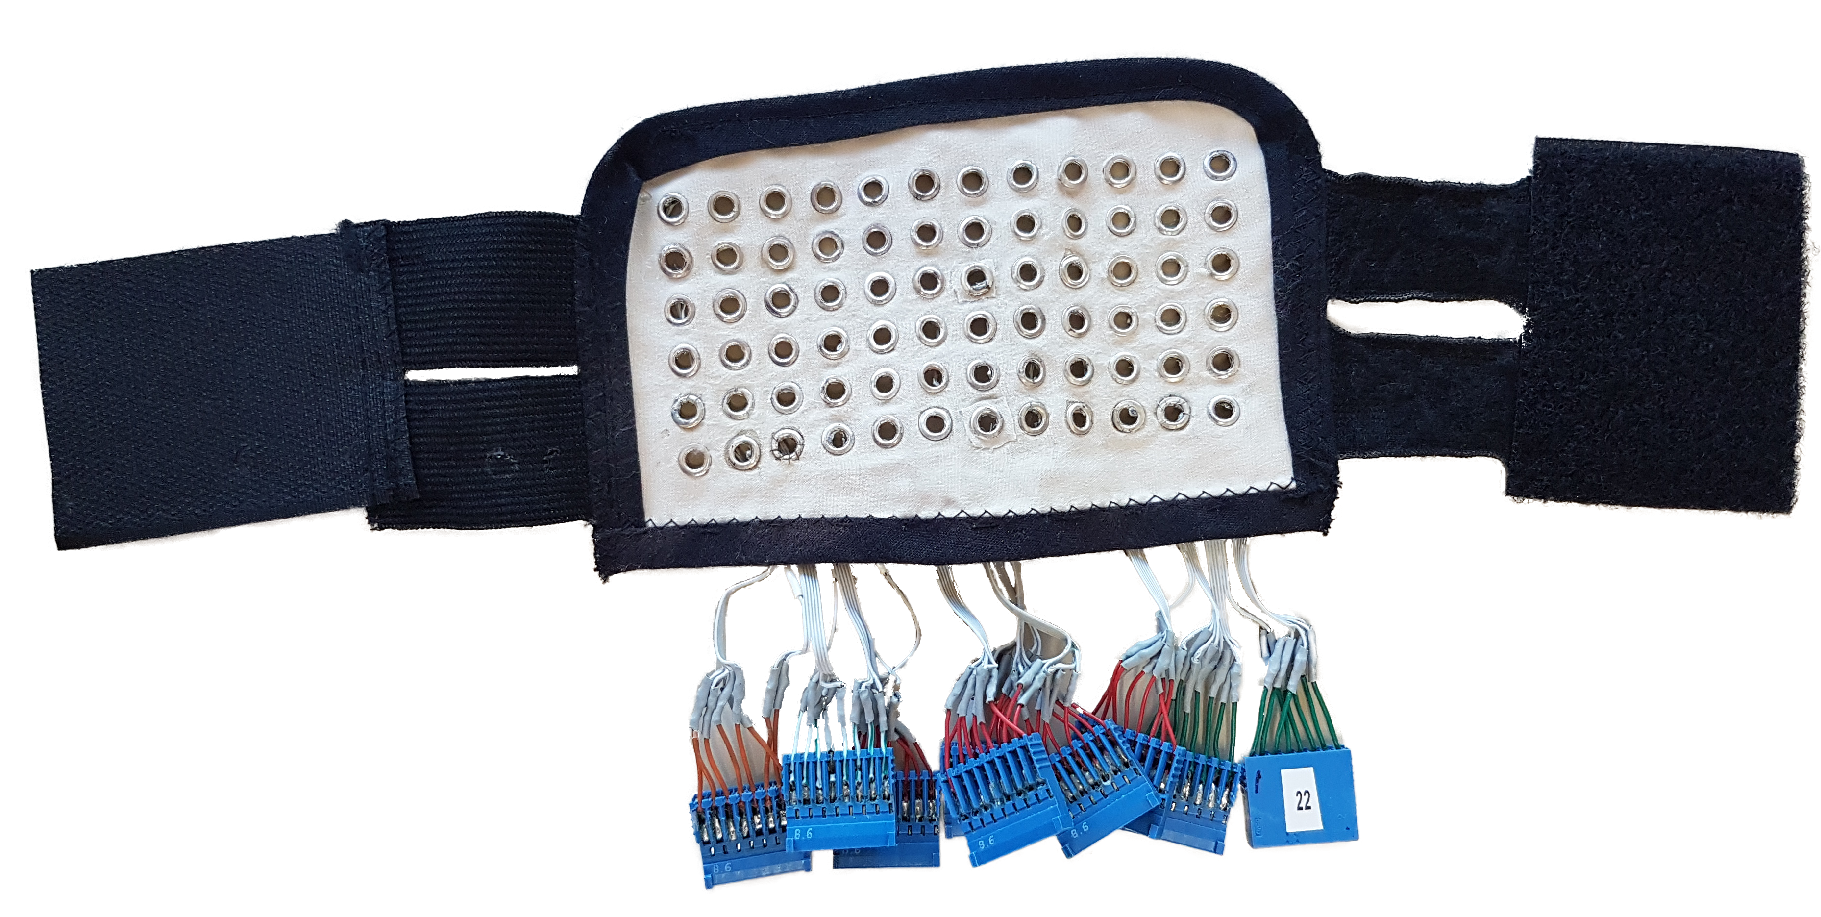
\includegraphics[width=0.7\textwidth]{Images/introduction/electrode2.png}
\caption{The figure represents HD-EMG electrode that was used for recording of database used in this Thesis.}
\label{fig:electrode}
\end{figure}

In addition, activation of individual motor units, i.e. individual motor neuron spike train, can be extracted from the HD-EMG recordings using Blind Source Separation methods \citep{Holobar2007, Holobar2010}, which can be a valuable information in force estimation because motor unit recruitment and firing frequency depend primarily on force level \citep{Merletti-book}. Several authors have used this approach instead of the traditional one based on intramuscular (invasive) EMG. One of the obvious advantages of this method is that is safe and not painful, although it has not been implemented in clinical practice yet. Using this technique, Holobar et al.  \citep{Holobar2010} were able to extract 6 to 7 motor units starting from contractions at 5\% MVC and up to 20\% MVC with associated discharge rates between 10 pps and 12 pps. However, one of the current limitations is that the intensity of isometric contraction must remain constant during the measurement.

HD-EMG recordings also allow calculation of two-dimensional activation maps where intensity of each pixel represents the intensity of a corresponding EMG channel (see figure \ref{fig:HD-EMG}). Consequently, the information on spatial distribution of EMG intensity over the muscle is provided. Recent studies show that changes in spatial activation pattern are related to duration of movement and fatigue \citep{Tucker2009, Staudenmann2014}, position of joint \citep{Vieira2010} and the level of contraction \citep{Holtermann2005}. 
\begin{figure}[ht]
\centering
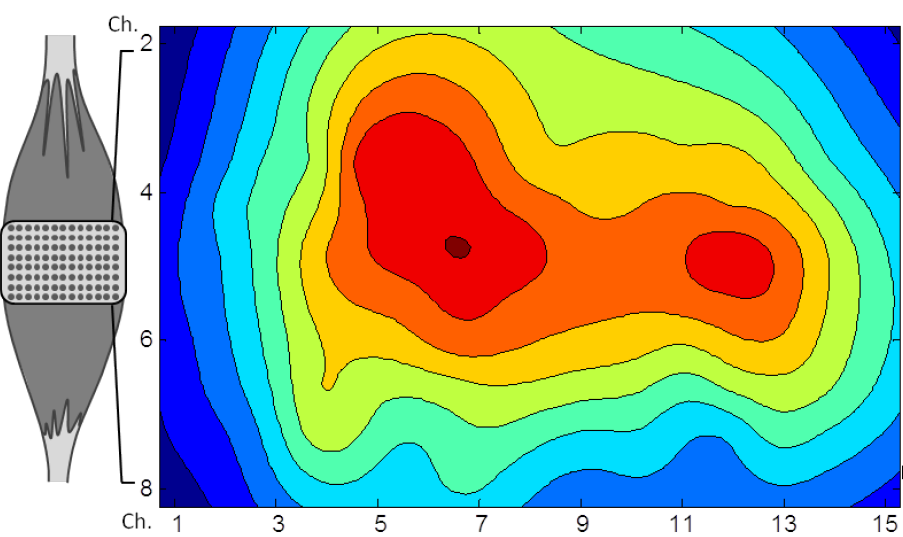
\includegraphics[width=0.95\textwidth]{Images/introduction/HD-EMG.png}
\caption{The figure represents the HD-EMG activation map recorded on the biceps brachii muscle during flexion. Distinct activation of the two heads can be noticed in the map. Modified from \citep{Monica-thesis}}
\label{fig:HD-EMG}
\end{figure}

These HD-EMG activation maps can be also used to determine multiple innervation zones \citep{Marateb2016}, but it was also proven that this spatial characteristics of HD-EMG change depending on the  task, but also depending on the force the subject is applying, and form repeatable muscle activation pattern that can be used in identification of motion intention \citep{Rojas-Martinez2012}.

However, HD-EMG can be corrupted by low quality channels, which are a common issue in measurements due to well-known artifacts, such as: electrode displacement, bad electrical contact between skin and the electrode, movement of cables, electromagnetic interference, etc. \citep{Clancy2002b}. Affected channels differentiate themselves in amplitude and spectral content. To cope with this problem, authors in \citep{Rojas-Martinez2012} developed an expert system for detection, removal and interpolation of HD-EMG channels corrupted by artifacts. On the other hand, Ghaderi and Marateb \citep{Ghaderi2017} used image inpainting and surface reconstruction methods to reconstruct the corrupted activation map.


\section{Task identification using pattern recognition}

Given the one to one relationship between the neural commands and the activation of motor units in the muscles, surface electromyography (sEMG) has been used for more than a half of century as a noninvasive and natural way of extracting motor control information for identification of motion intention. Such information is used in numerous applications in rehabilitation engineering, e.g., prosthetics \citep{Li2010, Young2013, Stango2015}, exoskeletons \citep{VacaBenitez2013} and rehabilitation robots \citep{Dipietro2005, Marchal-Crespo2009}.

Ideally, an identification system should fulfill the following criteria \citep{Farina2014}:
\begin{itemize}
\item Intuitive control: simultaneous and proportional
\item Insensitive to changes in electrode - skin impedance,
\item Adaptive to changes during the use, i.e. fatigue, electrode-skin impedance change due to sweating and drying of conductive gel
\item Insensitive to precise position of electrodes
\item Fast and easy training procedure (ideally none)
\item Real time identification, i.e. time delay less than 300 ms \citep{Oskoei2007}
\item Low computation complexity which enables implementation in battery-powered device
\end{itemize}

In most of the commercial prosthesis \citep{Parker1986}, sEMG of two muscles is recorded. In this simple scheme a single Degree-of-Freedom (DOF) can be controlled: the EMG amplitude of one muscle controls the output of one direction, whereas the EMG amplitude of the other muscle controls the other direction. If prosthesis needs to operate in multiple DOFs, a subject needs to switch between currently active DOF either by co-contraction or by pressing a switch button. In any case, the method is not intuitive nor efficient for the user \citep{Farina2014}.

Pattern recognition is an alternative to conventional control algorithms and has been extensively used in research institutions during last decades \citep{Hakonen2015, Farina2014}. The prerequisite of using pattern recognition for task identification is the presence of a pattern that can be extracted from the EMG signal. Major advancement over conventional switching myocontrol is the possibility of instant selection of one of predefined movements.

However, although pattern recognition improves the possibilities of extraction of motion intention, it has serious limitations. Therefore, there is still a large gap between use of pattern recognition in research and in practice in rehabilitation institutes and in users' homes \citep{Jiang2012}. Pattern recognition approach does not support proportional and simultaneous control for multiple motor tasks. Therefore, consecutive tasks need to be performed sequentially. This type of control prevents the user from achieving a fluid movement, but also demands planning of movement execution. There have been solutions proposed in literature that enable simultaneous controls over multiple degrees of freedom. For example, Young et al. \citep{Young2013} propose system of parallel classifiers that use conditional probabilities to separate between combination of tasks. On the other hand, there are also publications proposing solutions for proportional control. Fougner et al. prepared a review on the topic \citep{Fougner2012}. The main idea behind this technology is that the muscle force can be estimated using the EMG signal \citep{Staudenmann2010}. 

On the other hand, one of the disadvantages of pattern recognition is the fact that in spite of the high accuracy, an error could lead to the completely unwanted task. Furthermore, although identification rate is usually very high during the stationary task, errors often occur during transition between tasks. This problems can be partially prevented by employing the e.g. majority voting principle \citep{Englehart2003}, or decision-based velocity ramp that attenuates the velocity of a movement after the change of a task \citep{Simon2011}. % Englehart 300 ms

Although crosstalk is usually considered as a negative interference in electromyography, if it is consistent and repeatable, some authors argue that it can provide a discriminative power for task identification \citep{Farina2014}. However, for some approaches it has a negative influence \citep{He2015}. To resolve this issue, source separation methods can be used to separate EMG activity of adjacent muscles \citep{Farina2004, Holobar2014}. This can be a powerful tool in task identification \citep{Naik2007}, because it could separate contributions of individual muscles in the myoelectric signal, and, therefore, minimize crosstalk effect from nearby muscles. Consequently, extracted features would characterize only the target muscles.


According to Oskoei et al. pattern-recognition-based task identification approach includes four main modules \citep{Oskoei2007}:
\begin{description}
\item[Data segmentation:] \hfill \\
Comprises various techniques and methods that are used to handle data before feature extraction. Recording must be divided in time segments on which identification will be performed. Selection of duration of time segment has effect on the identification. Features calculated on wider segments usually have lower variability and, consequently, higher repeatability and stronger pattern, which increases identification rate. On the other hand, the output of the classifier should be as fast as possible in order to be used in real time.  Therefore, the shorter the window, the shorter the response time will be. General recommendation is that the delay should be less than 300 ms \citep{Oskoei2007, Englehart2003}. 
\item[Feature extraction:] \hfill \\
This module computes and presents preselected features for a classifier. Features, instead of raw signals, are fed into a classifier to improve classification efficiency. Selection or extraction features is one of the most critical stages in myoelectric control design.
\item[Classification:] \hfill \\
A classification module recognizes signal patterns, and classifies them into predefined categories. Due to the complexity of biological signals, and the influence of physiological and physical conditions, the classifier should be adequately robust.
\item[Controller:] \hfill \\Generates output commands based on signal patterns and control schemes. Post-processing methods, such as majority voting, which are often applied after classification to eliminate destructive jumps and make a smooth output, are included in this module too.
\end{description}

Many studies agree that selection of pattern recognition technique does not have a big influence on the task identification \citep{Hakonen2015}. Therefore, simple and fast classifiers are preferred. Linear discriminant analysis has become the 'gold standard' in the field of myoelectric control because of this properties \citep{Tkach2010, Li2014, Hakonen2015}. Although this classifier assumes multivariate normal distribution of classes, experiments proved that it performs well if when normality assumption is not met \citep{Grouven1996}. Features, on the other hand, have a major influence on the identification results \citep{Englehart1999, Tkach2010}. Therefore, there are many features proposed in the literature focused on improving rate of identification of motion intention:

\begin{description}
\item[Time domain features:] \hfill \\
Mean absolute value \citep{Hudgins1993}, integrated EMG \citep{Park1998}, variance \citep{Park1998, Zardoshti1995}, root mean square \citep{Farrell2008}, waveform length \citep{Hudgins1993}, zero crossing \citep{Hudgins1993}, log detector \citep{Tkach2010}, Wilson amplitude \citep{Zardoshti1995}, slope sign change \citep{Hudgins1993}, autoregressive coefficients \citep{Hargrove2007}, cepstral coefficients \citep{Park1998}, mean absolute value slope \citep{Phinyomark2012}, histogram of EMG \citep{Phinyomark2012, Zardoshti1995}
\item[Frequency domain features:] \hfill \\
Mean frequency \citep{Phinyomark2012b}, median frequency \citep{Phinyomark2012b}, modified mean frequency \citep{Phinyomark2009}
\item[Time-frequency domain features:] \hfill \\
Short time Fourier transform \citep{Englehart2003b, Englehart2001}, continuous wavelet transform \citep{Englehart2003b, Englehart2001}, discrete wavelet transform \citep{Englehart2003b}, stationary wavelet transform \citep{Englehart2003b}, wavelet packet transform \citep{Englehart2003b, Englehart2001, Chu2006}
\item[Spatial domain features:] \hfill \\
Experimental variogram \citep{Stango2015}, center of gravity \citep{Rojas-Martinez2012, Rojas-Martinez2013}
\end{description}

Time domain features are commonly used because they achieve high identification accuracy and are computationally efficient \citep{Hakonen2015}.

Since spatial distribution contains a lot of information on the muscle, it is acknowledged as a valuable feature in identification of motion intention \citep{Stango2015, Hakonen2015, Rojas-Martinez2013}. For example, Stango et al. \citep{Stango2015} used spatial characteristics of HD-EMG recording of the forearm muscles to identify 8 hand and wrist tasks (4 degrees of freedom). They fed support vector machine classifier with a statistical measure of spatial correlation, i.e. variogram and achieved high identification results (95\% accuracy). Furthermore, they proved that proposed spatial features are robust to electrode shift.

Most of pattern recognition identification methods are subject-specific. They usually achieve very high identification results, but require time consuming training procedure for every patient individually. This could be avoided by building a single identifier for a group of patients, i.e. group-specific identifier. However, inter-subject variability is a big concern in design of a group-specific pattern recognition-based identifier. Individuals differ from each other in a lot of physiological parameters, e.g., conductivity of subcuntaneous tissue, and limb dimension. Nevertheless, by comparing HD-EMG activation maps between normal subjects it has been shown that inter-subject activation patterns exists for different tasks and levels of contraction \citep{Rojas-Martinez2012}.

In \citep{Rojas-Martinez2013} authors demonstrate that by using intensity and spatial features extracted from activation maps it is possible to construct an inter-subject identification method based on LDA classifier not only for different tasks, but also for different effort levels. Authors reported that in healthy subjects identification performance improves by adding spatial features in the identification, which proves that spatial distribution is less sensitive to inter-subject variability. They achieved sensitivity higher than 75\% for identification of four upper-limb tasks at three different effort levels and more than 90\% sensitivity when identifying only four tasks and no effort level. Also, they report higher classification results when using classification in two steps (in first step task is classified, and in the second step level of effort), rather than a single step classification.


\section{Application to patients with neuromuscular impairment}

Physical injury to the brain, spinal cord, or nerves, is usually the cause of neurological disorders. According to World Health Organization, each year there are 500 000 spinal cord injuries and 15 million strokes (of which 5 million result with death and 5 million with permanent disability) every year. Furthermore, number of people who are older than 60 years will increase to 22\% of the world population by 2050 and will count 2 billion people. Unfortunately, in affected patients motor control can be impaired as a result of damaged nerves and they often suffer from uncoordinated movements, lack of force, and spasticity. On the other hand, stroke is a serious life-threatening condition that occurs when the blood supply to the brain is interrupted, resulting in severe disability among survivors. Brain damage due to stroke can affect important areas that control everything we do, including how we move different parts of our body. Common manifestations of upper extremity motor impairment include muscle weakness, impaired motor control, and changes in muscle tone are common manifestation of upper extremity motor impairment. These impairments induce disabilities in common daily life tasks like reaching and holding objects. During recovery process, rehabilitation robots that stimulate neuroplasticity are commonly used \citep{VacaBenitez2013, Dipietro2005, Marchal-Crespo2009}. 

Patients can still have uncoordinated movements, and lack of force, or, in more difficult cases, they can weakly activate their muscles, but cannot perform the movement. If their motion intention could be extracted in real time, it would allow them to control assistive devices and maximize the benefits of robotic-aided therapies where it has been proved that the active participation improves the medical condition of the patient \citep{Hogan2006}.

It was already shown that intensity-related and task-specific activation patterns exist in patients with neurological disorders and that motion intention can be extracted from EMG. In other words, movement that patient is trying to perform can be predicted using the recorded myoelectric activity. Liu and Zhou were able to successfully perform identification of tasks using time domain and autoregressive model features in patients with incomplete spinal cord injury \citep{Liu2013}, whereas Zhang and Zhou identified tasks in patients with stroke using a similar feature set \citep{Zhang2012}.

After the neurological disorder, rehabilitation treatment should start as soon as possible, only days after injury in stroke, whereas in case of spinal cord injury, after the inflammation. Early interventions can achieve incredible results and patients can either regain control of limbs, which is known as \emph{true recovery}, or can learn new compensatory movements, which is called \emph{restitution}. 

In spite the correct neuromuscular activation, patients sometimes cannot achieve movement because of insufficient contraction force, or spasticity \citep{Liu2016b}. These patients have good chance of recovery, but therapists are often unaware of their state. On the other hand, rehabilitation robots are mostly based on force and inertia, and, therefore, cannot be of assistance either. Since this patients have the ability to generate EMG signals, they could control a rehabilitation robot and maximize their chance of recovery by individualizing rehabilitation.




\section {Doctoral thesis overview}

This Doctoral Thesis is presented as the compendium of three publications. The topic of the Thesis is the analysis of muscular patterns of upper-limb muscles during isomeric contractions and its relationship to incomplete spinal cord injury. Furthermore, method for the identification of motion intention is developed base on pattern recognition approach and muscle co-activation patterns. 

The Doctoral Thesis is organized by chapters as follows:

\begin{itemize}
\item \textbf{Chapter 2: Problem statement}\\
	This chapter states the problem and provides the objectives of Doctoral Thesis.
	
\item \textbf{Chapter 3: Spatial distribution of HD-EMG improves identification of task and force in patients with incomplete spinal cord injury}\\
	This chapter represents the first publication of the compendium of publications. Using spatial distribution of myoelectric intensity task identification was performed on patients with incomplete spinal cord injury. This work proves the positive contribution of spatial features in pattern recognition technique of identification of motor tasks. Not only that the identification rate increases, but the features show resilience to slow time dependent changes in the myoelectric signal, such as fatigue and drying of electrolytic gel.
	
\item \textbf{Chapter 4: Prediction of isometric motor tasks and effort levels based on high-density EMG in patients with incomplete spinal cord injury}\\
	In this publication, the similarity of intensity and spatial distribution of intensity was investigated between patients with incomplete spinal cord injury. The results show that the repeatable pattern exists between different patients and, moreover, for the patients with similar level of injury this patterns are more similar.

\item \textbf{Chapter 5: A Novel Spatial Feature for the Identification of Motor Tasks Using High-Density Electromyography}\\
	This chapter summarizes the  third publication of the compendium. The novel feature was designed for task identification. It is based on probability density function of HD-EMG activation maps. Classifier based on this new feature show higher identification rate, as well as fidelity to fatigue.

\item \textbf{Chapter 6: Conclusions}\\
	In the last chapter, the conclusions and main contributions of the Thesis are provided. Also, the guidelines for the future work are stated, as well as list of publications derived from the Thesis.

\end{itemize}





\


%\chapter{Problem statement}

\narrowlinespacing
\begin{myquote}
\begin{flushright}
\textit{To define is to limit.} \\-- Oscar Wilde
\end{flushright}
\end{myquote}
\normallinespacing

Extraction of information on motor task intention can be used in many different applications from assistive devices, prosthetics, and rehabilitation robots to leisure and gaming equipment. This information can be extracted at any point of the system for motor control: from the brain centers controlling the movement to the muscles performing the movement. The central nervous system is organized in multiple levels, from simple connections between cells to coordinated cell populations, building a complex architecture of interconnected brain regions, including the centers for motor control. All this brain activity is summed together and its electromagnetic field can be measured on the scalp surface (electroencephalography, EEG). If this information is used as an interface between the subject and the computer, it is called the \emph{brain-computer-interface} (BCI). Although this approach is being extensively researched and the possibilities and achievements are rising rapidly, it is not an easy task. The problem is that the activity of the entire brain is superimposed to the motor control activity, such as emotions and memory.

On the other hand, EMG records electrical activity of many muscle units that carry similar information. The ratio of power of a useful signal, compared to the interference of other sources is much higher in the EMG recordings. Moreover, by recording myoelectrical activity over muscle surface with high spatial sampling (HD-EMG), even higher SNR can be achieved and more information can be extracted. Therefore, this doctoral thesis investigates the possibilities of extraction of motor control information from multichannel sEMG during voluntary contractions.

    
    
    \section{Motivation}
    
    Voluntary movements are achieved by the contraction of skeletal muscles controlled by the Central and Peripheral Nervous system. The contraction is initiated by the release of a neurotransmitter that promotes a reaction in the walls of the muscular fiber, producing a biopotential known as the Motor Unit Action Potential (MUAP) that travels from the neuromuscular junction to the tendons. The surface electromyographic signal records the continuous activation of such potentials over the surface of the skin and constitutes a valuable tool for the diagnosis, monitoring and clinical research of muscular disorders. Moreover, the use of electrode arrays facilitates the investigation of the peripheral properties of the active motor units such as: conduction velocity and fatigue \citep{Soares2015}; anatomical characteristics in terms of location of the innervation zones \citep{Beck2012}, the spatial composition of the muscle, that is, muscle compartmentalization \citep{Vieira2010}; estimation of number, type and spatial distribution of muscle fibers \citep{Marateb2016}; and change in spatial distribution of MUAPs with exercise and pain \citep{Madeleine2006}. This last property of the muscles has proven to be very useful to infer motion intention not only regarding the direction of the movement but also its force \citep{Rojas-Martinez2013}. The advantages of the HD-EMG lie in the large amount of recorded information, which enables minimizing the effect of electrodes shift and allows choosing an appropriate subset of channels for further analysis.  
%     HD-EMG also enables estimation of number, type and spatial distribution of muscle fibers \citep{Marateb2016}. This last property of the muscles has proven to be very useful to infer motion intention not only regarding the direction of the movement but also its force \citep{Rojas-Martinez2013}.
    %
%    HD-EMG enables measuring of valuable information about muscle unit recruitment: muscle fiber conduction velocity, location of the innervation zones, estimation of muscle fatigue, and estimation of number, type and the spatial distribution of muscle fibers \citep{Marateb2016}. The advantages of the HD-EMG lie in the large amount of recorded information, which enables minimizing the effect of electrodes shift and allows choosing an appropriate subset of channels for further analysis.
    
%Spinal cord injury is a neurologically disabling disease like the stroke.
In this thesis muscle co-activation patterns will be analyzed both in healthy subjects, and in patients with incomplete spinal cord injury (iSCI). In these types of neuromuscular impairments, patients often have residual motor capabilities and can weakly activate their muscles. However, although muscle is contracting and generating myoelectrical activity, the contraction is sometimes insufficient to generate joint movement. In this situation, it is likely that the rehabilitation will not be successful and the patient could develop compensatory movements to replace the lost functionality, either by himself, or by following the therapist's advice. Moreover, rehabilitation robots are widely used in this type of rehabilitation care. However, robots most often have only force sensors and can adjust the trajectory depending on the force that the patient is producing in order to assist/resist his efforts. Although it is well known that rehabilitation robots have a positive effect on the therapy, their effect on the rehabilitation could be greatly improved if the robots would adjust the force and trajectory based on the patient's capabilities and efforts. A patient's effort to achieve the movement could be extracted by a HD-EMG myocontrol system, which would be connected into the feedback loop of the robot to personalize the rehabilitation. It has been proven already that simple movement of a patient's limb along a set trajectory has a minimal effect on the outcome of the therapy and that the therapy can be greatly improved if the patient is actively trying to achieve a movement. Therefore, a personalized therapy system that responds to the patient's movement intention could bring recovery and patient's independence.

To achieve the accurate identification of motion intention using pattern recognition, a repeatable co-activation pattern should be present among the patients with neurologically disabling diseases. Therefore, the reproducibility of specific muscular activation patterns was investigated in patients with incomplete spinal cord injury during four isometric tasks of the upper limb, paying close attention to the spatial activation patterns. Moreover, activation patterns were also analyzed during different levels of effort.

Muscular pattern reproducibility can be evaluated using a pattern recognition techniques for task identification. In other words, results of task identification can be used as a figure of merit for muscular pattern quality. If the features extracted from the HD-EMG signal form a distinct pattern for each of the tasks, and if patterns for different tasks are different, identification performance will be high, that is, recognizable and distinct patterns will yield high identification results.
   
Task identification using pattern recognition consists in classification of the recorded sEMG signal segments into one of predefined classes based on a set of characteristics, i.e., pattern, extracted from the recorded EMG signal. These extracted features should ideally form a repeatable and distinct pattern for each class, and should be different between classes. A variety of classifiers (e.g. hidden Markov models, support vector machine, artificial neural network, fuzzy logic and linear discriminant analysis) \citep{Oskoei2007} have already been employed in myocontrol research. Nevertheless, multiple authors agree that the identification does not depend much on the classifier type \citep{Hargrove2007, Zhang2012, Hakonen2015}. Therefore, simple and easy to train classifiers like linear discriminant analysis are preferred \citep{Li2010, Englehart1999, Tkach2010, Li2014, Hakonen2015}. On the other hand, finding an appropriate set of features is challenging \citep{Englehart1999, Tkach2010, Liu2013}.

Through this thesis, the linear discriminant analysis (LDA) was used as a pattern recognition classifier, whereas the support vector machine (SVM) was used for the comparison in only one publication. LDA is a computationally simple and efficient classifier with linear decision boundary and it is based on the Bayesian equation \citep{McLachlan2004}. It is a \emph{parametric classifier}, i.e., it estimates statistical probability of classes by estimating the probability density function of each class from the available data, which is not a simple task and can often be erroneous. On the other hand, SVM \citep{Cortes1995} is nowadays known as a very powerful classifier with a lot of different applications. The big advantage over LDA is the fact that it is a \emph{non-parametric} classifier. The model of the classifier is not obtained using assumptions of the form of the class density function and estimation of it's parameters, which is inevitably a source of error. Instead, SVM forms the decision boundary using the samples (not their density estimates) by maximizing the distance between samples and the boundary. This was the idea Vladimir Vapnik, the inventor of this method stood for. It is better to try to solve the problem directly and simply, without many intermediate steps that can often be complicated and inaccurate. Detailed explanation and the working principle of these two classifiers are provided in the appendix \ref{pattern_recognition}.

The challenges faced in pattern recognition in electromyography include many factors, such as electrode shift \citep{Hargrove2008, Young2011}, change in arm posture \citep{Fougner2011}, and slow time dependent changes \citep{Farina2014}. This thesis addresses the challenges caused by slow time-dependent changes like fatigue \citep{Tkach2010} and change in electrode-skin impedance \citep{Clancy2002b} on highly controlled isometric tasks. A patient's limb was held in place during measurements using a mechanical brace in order to restrict joint movement. Therefore, effects accounted for limb movement, that is, electrode shift and change in arm posture, were minimal.  


     \section{Objectives}
     
     	\subsection*{Main objective}

This doctoral thesis addresses the problem of extraction of information from muscular patterns obtained from multichannel surface electromyography and associates them with different motor tasks and effort levels. The aim of the thesis is to analyze the muscular pattern of the upper-limb muscles during isometric contractions and its relationship to neuromuscular disorders, namely to incomplete spinal cord injury. This information can be useful for the identification of motion intention, i.e. identification of the intended motor task and force based on the sEMG, and could provide a control signal to interfaces that control external devices, like exoskeletons or rehabilitation robots, particularly for patients with neuromuscular disorders including spinal cord injury.

      
        \subsection*{Specific objectives}
        
To achieve the main objective, this thesis strives for the following specific objectives:

\begin{enumerate}[I]

\item To investigate muscle co-activation patterns extracted from multichannel sEMG in patients with incomplete spinal cord injury during isometric contractions, as well as to evaluate the repeatability of the muscular patterns for different motor tasks, and for different effort levels. The patterns related to intensity and spatial distribution of intensity were evaluated.

\item To investigate the influence of myoelectric fatigue on the obtained patterns and the effect on the task identification.

\item To investigate how these patterns change during recording time due to non-physiological parameters like drying of conductive gel.

\item To search for the similarity in multichannel sEMG activation patterns between different patients with incomplete spinal cord injury using the pattern-recognition approach.

\item To define new spatial features, test them in the identification of task and force of isometric contractions using pattern recognition, and to test the robustness of such features to physiological and non-physiological changes.

%\item To publish the obtained results and conclusions in high-impact journals and conferences.

\end{enumerate}

     \section{Thesis framework}
     
This thesis and the published articles that provide its content as a compendium were developed in the \emph{Department of Automatic Control (ESAII)} of the \emph{Universitat Polit\`{e}cnica de Catalunya (UPC)} under the framework of the muscular research line of the \emph{BIOsignal Analysis for Rehabilitation and Therapy Research Group (BIOART)}, that is part of the \emph{Biomedical Signals and Systems} division of the \emph{Biomedical Engineering Research Centre (CREB)} of UPC and the Biomedical Research Networking Center in Bioengineering, Biomaterials and Nanomedicine (CIBER-BBN). The research was done in collaboration with the \emph{Laboratory of Engineering of Neuromuscular System and Motor Rehabilitation} at the \emph{Politecnico di Torino}, directed by prof. Roberto Merletti, and with the \emph{Institut Guttman} in Badalona (Spain), where Ursula Costa and Josep Medina recruited the patinets.

Furthermore, this work has been supported by multiple funding projects and grants:

\begin{enumerate}
\item Ayudas para la contratación de personal investigador novel (FI-DGR 2014). \emph{Agencia de Gestión de Ayudas Universitarias y de Investigación (AGAUR) - Generalitat de Catalunya.}

\item 	Sistemas multicanal de análisis y sensorización para rehabilitación y monitorización clínica. (DPI2011-22680) \emph{Ministerio de Economia, Industria y Competitividad (MINECO)}

\item 	Design of methods for assessing processes of neurological and neuromuscular decline associated with aging. (DPI201459049R) \emph{Ministerio de Economia, Industria y Competitividad (MINECO)}


\end{enumerate}

\chapter[Spatial distribution of HD-EMG in task identification]{Spatial distribution of HD-EMG improves identification of task and force in patients with incomplete spinal cord injury }
\label{ch:3}
\textbf{Published as:} 
Jordanić, M., Roja-Martínez,  Ma\~nanas, M.A., Alonso J.F.
Spatial distribution of HD-EMG improves identification of task and force in patients with incomplete spinal cord injury \textit{Journal of NeuroEngineering and Rehabilitation} 13(1):41, 2016

doi: 10.1186/s12984-016-0151-8

Impact Factor: 3.222; Position: 3 of 65 (Q1) REHABILITATION, 12 of 77 (Q1) BIOMEDICAL ENGINEERING.


\change{You have to change this running title}
\textbf{Abstract:} \textit{Background.} Recent studies show that spatial distribution of High Density surface EMG maps (HD-EMG) improves the identification of tasks and their corresponding contraction levels. However, in patients with incomplete spinal cord injury (iSCI), some nerves that control muscles are damaged, leaving some muscle parts without an innervation.
Therefore, HD-EMG maps in patients with iSCI are affected by the injury and they can be different for every patient.
The objective of this study is to investigate the spatial distribution of intensity in HD-EMG recordings to distinguish
co-activation patterns for different tasks and effort levels in patients with iSCI. These patterns are evaluated to be used
for extraction of motion intention. \textit{Method.} HD-EMG was recorded in patients during four isometric tasks of the forearm at three different effort levels. A linear discriminant classifier based on intensity and spatial features of HD-EMG maps of five upper-limb muscles was used to identify the attempted tasks. Task and force identification were evaluated for each patient individually,
and the reliability of the identification was tested with respect to muscle fatigue and time interval between training and identification. \textit{Results.} Three feature sets were analyzed in the identification: 1) intensity of the HD-EMG map, 2) intensity and center of gravity of HD-EMG maps and 3) intensity of a single differential EMG channel (gold standard). Results show that the combination of intensity and spatial features in classification identifies tasks and effort levels properly (Acc = 98.8 \%; S = 92.5 \%; P = 93.2 \%; SP = 99.4 \%) and outperforms significantly the other two feature sets (\textit{p} \textless \,0.05). \textit{Conclusion.} In spite of the limited motor functionality, a specific co-activation pattern for each patient exists for both intensity, and spatial distribution of myoelectric activity. The spatial distribution is less sensitive than intensity to myoelectric changes that occur due to fatigue, and other time-dependent influences.

\textbf{Keywords:} Myoelectric control, Pattern recognition, High-density electromyography, Incomplete spinal cord injury


\section{Backround}

Surface electromyography (sEMG) is commonly used in noninvasive extraction of motor control information and identification of motion intention. Therefore, it has a wide practical application in rehabilitation engineering, e.g., prosthetics [1, 2, 3], exoskeletons [4] and rehabilitation robots [5, 6].

Conventional myocontrol is based on non-pattern recognition strategies. In a classical example of a single joint prosthesis (one degree of freedom), sEMG signals are recorded on two independent muscles. EMG of one muscle controls the intensity in one movement direction, and the EMG of another muscle in the opposite direction. The output force is proportional to EMG power of the controlling muscle. This strategy is simple, computationally efficient, robust, and does not need training, which makes it suitable for unsupervised, everyday use. However, it allows control only in one degree of freedom (DoF) at a time. Although this approach can provide intuitive interface with fewer commands [7], in case of a prosthetic device with multiple degrees of freedom (e.g. hand prostheses), switching between DoFs is impractical and requires a long time to complete a complex task [8].

On the other hand, pattern recognition-based control strategy enables usage of multiple DoFs without switching, which significantly improves task completion time [7]. Although a variety of classifiers (e.g. hidden Markov model, support vector machine, artificial neural network, fuzzy logic) have been evaluated for task identification [9], multiple authors agree that the identification does not significantly depend on the classifier type [7, 10, 11]. Therefore, simple and easy to train classifiers, e.g. linear discriminant analysis (LDA), are preferred [12, 13, 14, 15]. Conversely, finding an appropriate set of features is challenging [16, 17, 18, 19]. Time-domain features are commonly used because they can achieve high identification results and are computationally efficient [7].

The technological advancement of EMG acquisition systems [20, 21] enables the use of high-density electromyography (HD-EMG). By using an array of closely spaced electrodes organized in a quadrature grid, a wide muscle area is recorded. This technology allows insights into the spatial distribution of the myoelectric intensity of a muscle. The spatial distribution allows monitoring the activation of different muscle regions, which depends on joint position [22], contraction level [23], and duration of movement [24]. In addition, it has already been reported that spatial features can be used in task identification in normal subjects [3, 25].

In patients with neurological disorders (e.g., stroke, spinal cord injury) motor control is impaired and some muscle parts can be left without innervation. As a result, patients often have problems with uncoordinated movements, lack of force, and spasticity. Rehabilitation and therapy can partially regenerate motor control, and either the affected muscles can recover partial functionality or other muscle groups can replace the functionality of a dysfunctional part. Therefore, the spatial distribution of motor unit action potentials is different from subject to subject and depends on the injury. But is it task-specific? And a more interesting question: is it force-specific? Liu \& Zhou [17] already proved that an intensity-related muscle co-activation pattern exists and that different hand tasks can be successfully identified in patients with incomplete spinal cord injury (iSCI). But can spatial distribution of myoelectric intensity help in identification of task and level of effort in patients with iSCI?

In this work, a method for the identification of different tasks and effort levels in patients with iSCI is proposed. High density EMG was measured on muscles participating in the analyzed contractions. By using different feature sets and an LDA classifier, we demonstrate that a specific co-activation pattern exists in patients with iSCI not only for a certain task, but also for a contraction intensity. Furthermore, the influence of time-dependent changes in EMG signal (due to muscle fatigue and drying of conductive gel) on the reliability of identification was evaluated. It was demonstrated that features related to spatial distribution not only improve the identification, but they are also more robust to time changes. What is more, they are helpful when identifying both the task and the desired force, indicating that spatial activation of motor units depends on type of exercise and contraction level in patients with iSCI.


\clearpage 
\section{Method}

\subsection*{Measurements}

\subsubsection*{Instrumentation}
\change{add fig1}
For the recording of HD-EMG signals, 2-D electrode arrays were fabricated in our laboratory (see Fig. 1c). They were designed as silver-plated eyelets (5 mm external diameter), embedded in a hydrophobic fabric in a quadrature grid with 10 mm inter-electrode distance. When positioned and fixed with elastic straps, fabric follows the contour of the muscle enabling a constant electrical contact between subject’s skin and eyelets.

%\begin{figure}[ht]
%\centering
%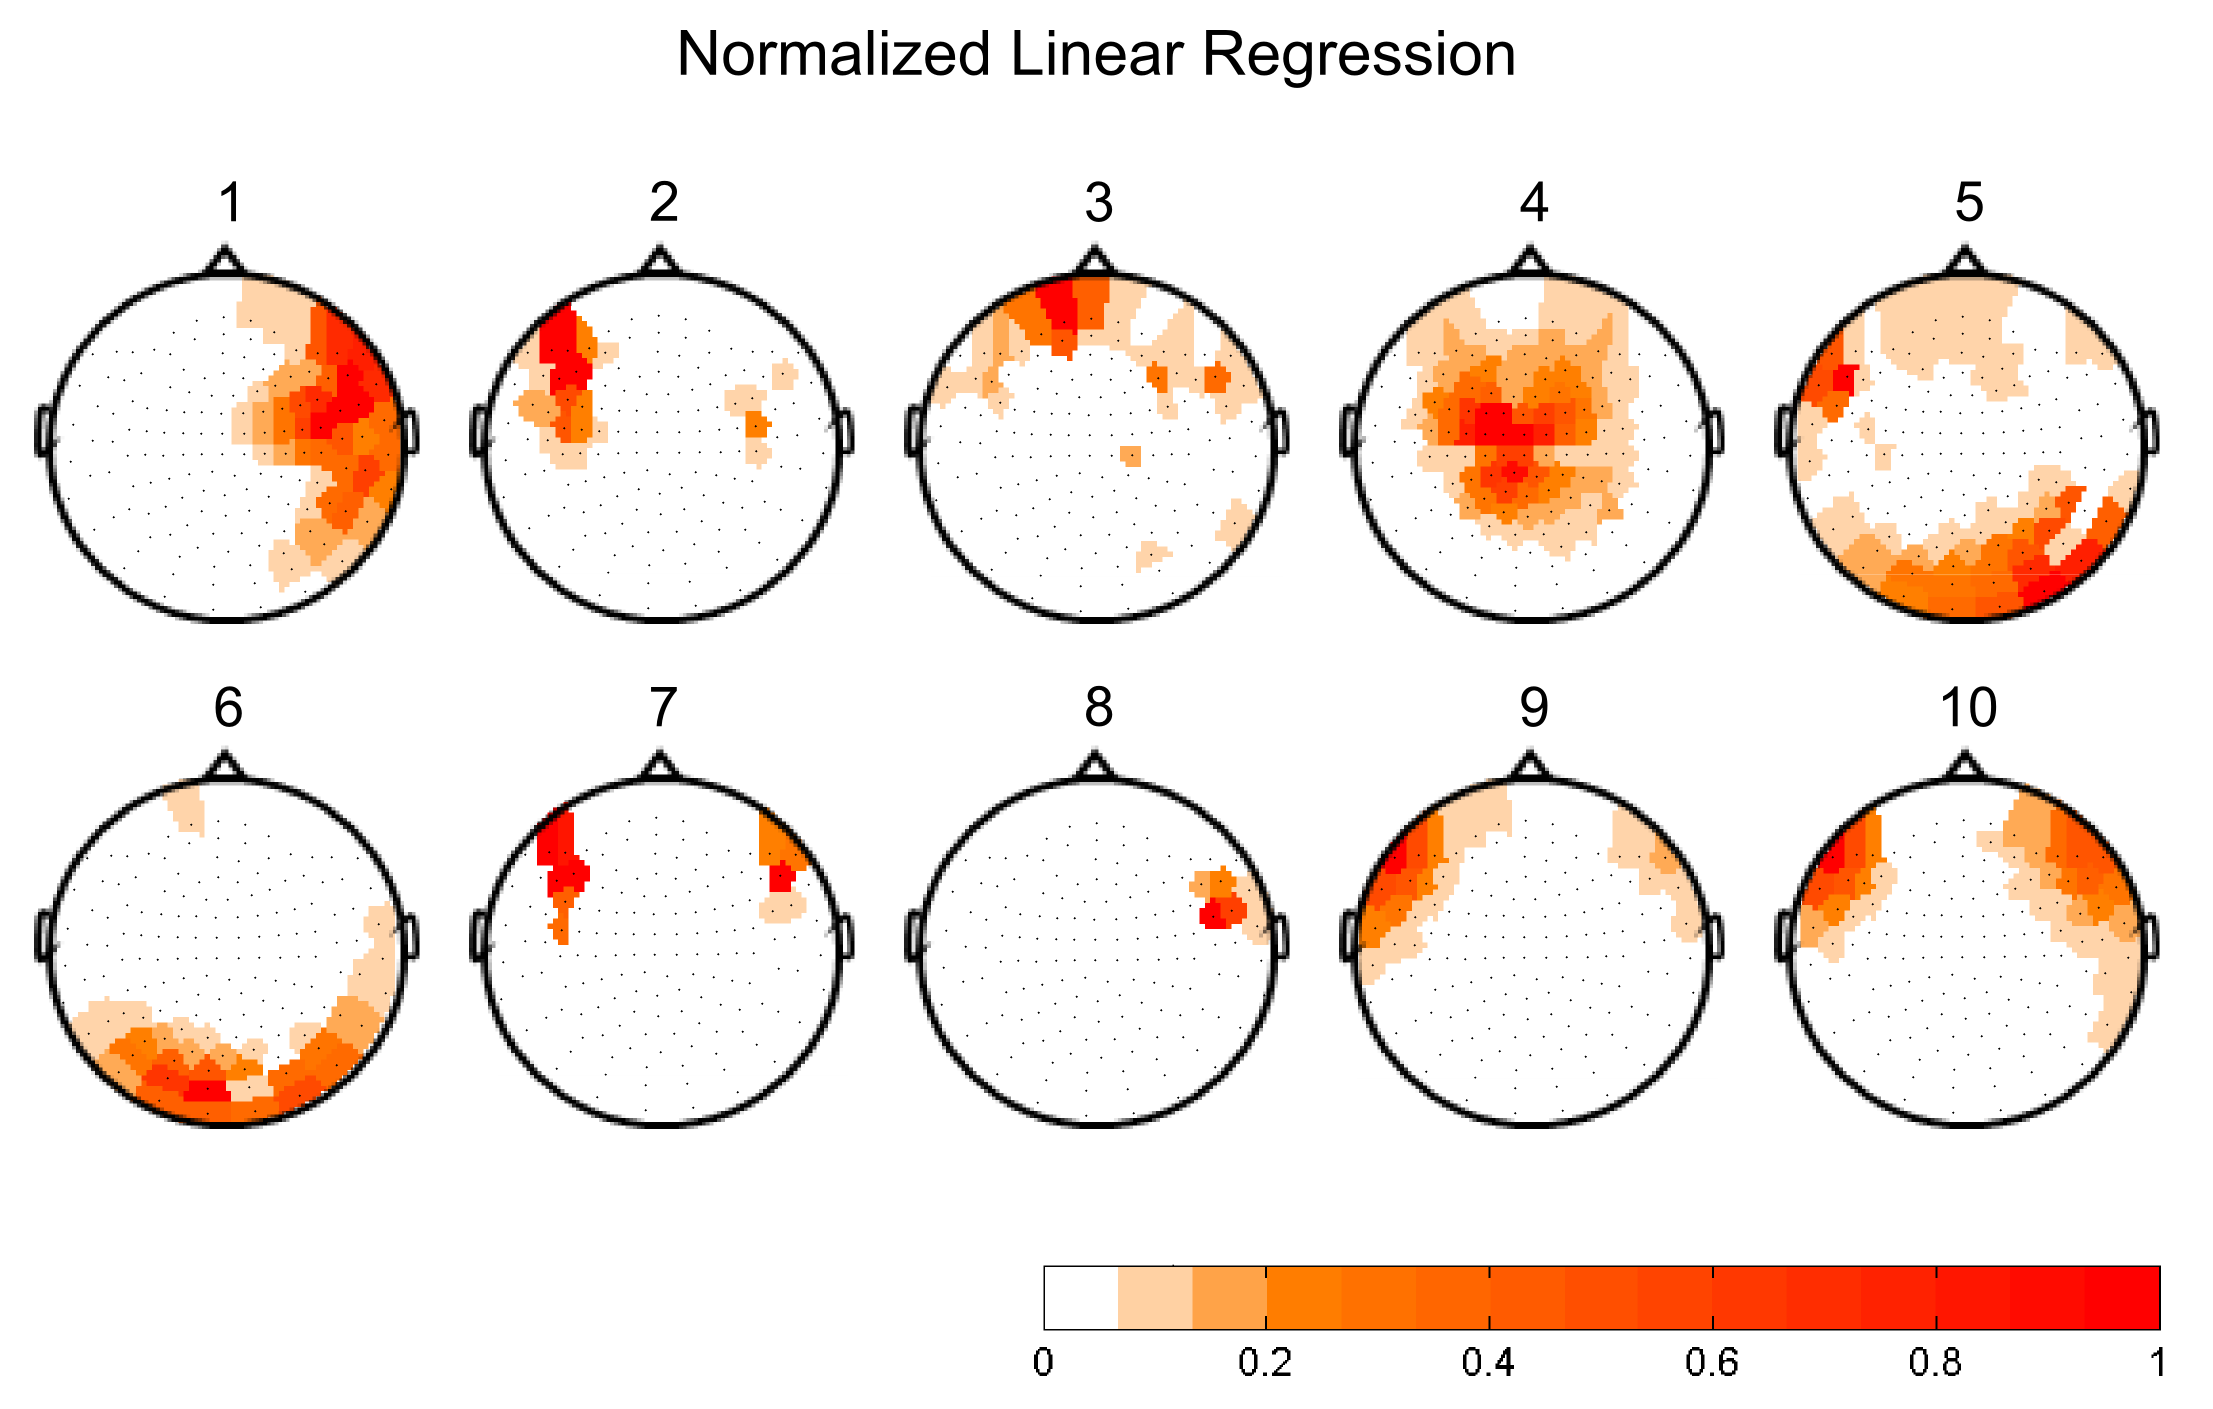
\includegraphics[width=0.9\textwidth]{Images/fig1-3.png}
%\caption{Sum of the linear regression coefficients normalized with respect to its maximum for all of the selected artifactual patterns for the 10 simulated MEG sets. Coefficients were obtained for the whole head after morphology selection and linear regression of each channel with the selected morphologies. Note that metallic artifacts behave differently depending on their nature and therefore they can appear in different areas of the head for each simulated MEG set.}
%\label{fig:1-3}
%\end{figure}      


In total, 240 monopolar EMG channels were recorded for each patient using three electrode arrays. A “driven right leg” circuit [26] was used to reduce the common mode interference by feeding the common mode voltage with opposite phase to the patient.

Monopolar EMG signals were digitized using two amplifiers with synchronized sampling (EMG-USB- 128 channels, sampling frequency 2048 Hz, 3 dB bandwidth 10–750 Hz, programmable gains of 100, 200, 500, 1000, 2000, 5000, 10000, manufactured by LISiN-OT Bioelettronica).

In order to perform isometric contractions at the desired force, a mechanical brace was used and torque transducers (OT Bioelettronica, range 150 Nm, resolution 2.5 mV/V) were placed on each joint to record the exerted torque (Fig. 1). During the measurements, patients were sitting upright in front of the brace with their dominant arm immobilized at the wrist to avoid hand grip. The forearm was in the sagittal plane, halfway between pronation and supination. The elbow was flexed at 45\textdegree and the shoulder was adducted at 90\textdegree in the horizontal plane and flexed at 45\textdegree in the sagittal plane. The exerted force level was displayed online to patients during the exercise for visual feedback.

\subsubsection*{Experimental setup}
Nine patients (four male, five female; age: 47 ± 18 years; body mass index: 28.2 ± 4.2) diagnosed with iSCI at C4-C6 levels participated in the study. Patients were rated C or D according to the ASIA scale and were injured at least 1 month before the experimental session. The study was conducted in accordance with the Declaration of Helsinki and subsequent amendments concerning research in humans and was approved by the Hospital Ethics Committee and the Local Government. All volunteers gave their written informed consent to participate.

HD-EMG was recorded during four isometric upper-limb tasks, i.e. flexion/extension of the elbow and supination/pronation of the forearm, on five superficial muscles involved by these tasks: Biceps Brachii, Triceps Brachii, Anconeus, Brachioradialis, and Pronator Teres. Prior to positioning of the electrode arrays, skin was cleaned, shaved, and treated with abrasive gel.

Three electrode arrays were used during the experiment: array A1 was placed over the forearm covering Anconeus, Brachioradialis and Pronator Teres muscles, and arrays A2 and A3 were placed over the upper arm covering Biceps Brachii and Triceps Brachii muscles. Reference electrodes were placed on the clavicle, wrist and shoulder of the active arm. After placing the arrays, each eyelet was filled with 20 μl of conductive gel using a gel dispenser (Multipette Plus, Eppendorf, Germany). The experimental setup can be seen in Fig. 1.


\subsubsection*{HD-EMG recordings}
Before signal recording, the maximal voluntary contraction (MVC) was measured for each task as a maximum of three consecutive trials. To prevent fatigue, each trial was followed by a three minute rest [27, 28]. Patients were trained to keep their fingers and wrist relaxed in order to minimize the activity of forearm muscles that do not participate in the intended tasks.

The measurement protocol was composed of two parts. In the first part, contractions at three levels of effort (10\%, 30\% and 50\% MVC) were measured for each task in randomized order. Visual feedback of the level of effort was provided in real time and subjects were asked to maintain the target level as precise as possible. Patients were instructed to remain at rest for three seconds followed by a contraction at a predefined force level for 10 s. There were three-minute breaks between consecutive recordings to prevent cumulative fatigue.

The second part of the measurement protocol began approximately half an hour (27.0 ± 9.8 min) after the end of the first part of the protocol. Each measurement started with a three-second rest period after which patients performed contraction at 50\% MVC until failure. The procedure was repeated for each task and between recordings there were three-minute breaks.
The recorded signals were divided into three sets for the subsequent analysis: the first set (submaximal set) was composed of the signals recorded in the first part of the protocol. The second set (time-effect set), used to test the time effect on the identification, was extracted from the beginning (up to 20\% of the total duration of the contraction, TDC) of the signals recorded in the second part of the protocol. Finally, the third set (endurance set) was used to test the effect of myoelectric fatigue on the identification, and was composed of the totality of the signals recorded in the second part of the protocol. The flow chart of the recording protocol can be seen in Fig. 2.



\subsection*{HD-EMG maps and feature extraction}
\subsubsection*{HD-EMG maps calculation}
Low quality channels, a common issue in HD-EMG measurements, were identified by an expert system proposed by Rojas-Martínez et al. [29]. The system is based on thresholds associated with the following three features: 1) relative power of low frequency components (from 0 to 12 Hz); 2) relative power of power-line components (50 Hz and first four harmonics); and 3) power calculated from RMS value of the signal. EMG channels without measurement artifacts were zero-phase filtered between 15 Hz and 350 Hz (Butterworth bandpass filter, 4th order), and the first 6 harmonics of power line coupling were suppressed by using the adaptive transversal filter described in [30], whose weights were estimated by a least mean squares algorithm.

HD-EMG maps represent the spatial distribution of intensities of active motor units over the surface of the muscle:
\change{Equation 1}

where HM is an activation map and each pixel in a map (HM i,j ) corresponds to an RMS value of a channel in an electrode array (position i,j). Maps were calculated on non-overlapping time windows of 250 ms to ensure an acceptable response time in applications directed to myoelectric control [9], and channels previously identified as artifacts were replaced by triangle-based cubic interpolation [29].


\subsubsection*{Feature extraction}
Two types of features related to HD-EMG maps were extracted: intensity and center of gravity. They were used in classification individually or combined in order to compare their performance. Additionally, the intensity of a single differential channel, i.e. traditional bipolar recordings usually employed in pattern recognition as a “gold standard”, was compared to other features. In any case, the feature set was composed of features extracted from all 5 monitored muscles.
Multiple studies suggest that the relationship between EMG amplitude and generated force is not linear [31, 32]. Accordingly, the intensity features were calculated as a common logarithm of the mean intensity of the HD-EMG maps, which proved to achieve higher classification results than a linear measure [25]:
\change{add equation 2}

where I is an intensity feature calculated from the HD-EMG intensity map HM with a total number of N channels, and HM ij is the intensity of a channel located at position i,j.

The center of gravity of an HD-EMG (CG) map was calculated as:
\change{add equation 3}
where (i,j) represents a channel position in the HD-EMG map HM.

The intensity of a single differential channel (Diff) was calculated as a common logarithm of an RMS value of difference of two consecutive channels in the direction of muscle fibers:
\change{add equation 4}
where the locations of channels (i,j) and (i + 1,j) are selected following SENIAM recommendations [33]. Diff was calculated on the same 250 ms time epoch as the HD-EMG map.


\subsection*{Identification of motion intention}
\subsubsection*{Classification}
Three LDA classifiers based on different feature sets extracted from all five monitored muscles were evaluated in the study:
\begin{enumerate}
\item Classifier based on the intensity of the HD-EMG map (I)
\item Classifier based on the intensity and center of gravity of the HD-EMG map (I + CG)
\item Classifier based on the intensity of a single differential channel (gold standard) (Diff)
\end {enumerate}

These classifiers were evaluated in the identification of task and level of contraction in patients with iSCI. Furthermore, the reliability of the classifiers was tested with respect to the slow time-dependent changes occurring in myoelectric signals, like those associated with gel drying or those related to changes at the physiological level (myoelectric fatigue).

Available observations were divided into a training group, which was used to train the classifier, and a validation group, which was used to evaluate classifier’s performance. Both groups were balanced, i.e. there was an equal number of observations of each class in the training group, as well as in the validation group, and data were split into training and validation sets using a 50\% / 50\% ratio [34]. To confirm the model was not overfitted, the results of classification of both sets were compared and were found similar. To achieve the statistical stability of results, each classifier was trained and evaluated in one thousand iterations, which are enough to avoid the potential error due to bad data partitioning [35], and then classification results were averaged. In every iteration, observations in the training and validation groups were assigned randomly.

The performances of the classifiers were expressed in terms of accuracy (Acc), sensitivity (S), precision (P) and specificity (SP) [36], as described in the following equations:
\change{add equation 5-8}

where true positives (TP) is the number of samples correctly appended to a certain class; true negatives (TN) is the number of samples that do not belong to a certain class and were not classified to that class; false positives (FP) is the number of samples not belonging to a certain class, but wrongly classified into that class; and false negatives (FN) is the number of samples belonging to a certain class, but wrongly classified into another class.


\subsubsection*{Short-term identification}
Classifiers with different sets of features (I, I + CG, and Diff) were tested on the submaximal set. Signals belonging to this set were recorded in a short time interval and, consequently, in the same conditions.

Two types of identification were considered: 1) Identification of tasks and 2) Identification of tasks and effort levels. Identification of tasks had 4 classes corresponding to the type of the task (flexion, extension, supination, and pronation) and an additional fifth class that corresponds to the rest period – no activity class (NoAct). Observations of no activity were extracted from the first three seconds of each recording, where subjects were asked to maintain at rest. Activity classes consisted of a mixture of all effort levels. On the other hand, identification of tasks and effort levels had 13 classes: 4 tasks with 3 levels of effort for each task (10\% MVC, 30\% MVC and 50\% MVC) and NoAct class.

Considering that patients were not always able to maintain the target level of contraction given their condition, the torque signal was used to select only time segments where the measured force remained within a threshold of ±5\%, ±10\% and ±10\% MVC for target contractions at 10\%, 30\% and 50\% MVC. From every submaximal contraction 20 non-overlapping, 250 ms time epochs, closest to the target force were selected. This procedure ensured 20 observations for each task with differentiation on the level of effort, or 60 samples for each task, without differentiation on the effort level. Consequently, 60 observations without muscle activity were selected for NoAct class from the beginnings of exercises (rest period).


\subsubsection*{Influence of time- progress on identification}
Wet electrodes with conductive electrolytic gel are commonly used for sEMG recording. However, these electrodes are not good for long-term monitoring [37]. Gel drying increases skin-electrode impedance, affecting amplitude and spectral content of the recorded signal. Moreover, skin perspiration is enhanced under the electrode array, which also affects the skin-electrode impedance and, consequently, the characteristics of the recorded signal. To compare the performances of the different features, task identification was tested in these conditions.

Classifiers were trained on the submaximal set and validated on the time-effect contractions recorded in the second part of the protocol. As in the previous section, 20 time epochs for each task and level of effort were identified from the submaximal set based on the torque signal. Half the extracted observations of all levels of effort were used for training, following the recommendations of Scheme and Englehart [12], where it was noticed that a mixture of effort levels in the training group yields a more robust classifier. NoAct observations for the training group were extracted from recordings in the first part of the measurement protocol, whereas observations for the validation group were extracted from recordings in the second part of the protocol.

For comparison, the same classifier was used to validate contractions recorded at the first part of the protocol, i.e. using samples of the submaximal set. Since the classifier was trained on just half of the available observations from the submaximal set, the remaining observations were used for validation. But considering that time-effect set was composed of contractions recorded at 50\% MVC effort level, the validation group was also composed only of 50\% MVC contractions from the submaximal set.

The classifier was trained and evaluated over 1000 iterations with observations selected randomly both in the training and validation sets to avoid bias in the performance.



\subsubsection*{Influence of muscle fatigue on identification}
Muscle fatigue is a slow change that occurs in contracting muscles. It alters the characteristics of recorded sEMG signal (i.e. amplitude and frequency content) [38] and, inherently, alters the extracted classification features [39]. To test the effect of fatigue on identification, each recording in the endurance set was divided into five equal time segments, i.e. 0–20\% TDC, 20–40\% TDC, 40–60\% TDC, 60–80\% TDC, and 80–100\% TDC. The first segments (0–20\% TDC) were used as a training group and the identification was carried out on all segments. The classification indices (accuracy, sensitivity, precision and specificity) were calculated for each segment in order to monitor performance during fatigue. The number of observations of each class was the same in the training group, as well as in the validation group.


\subsubsection*{Statistical methods}
A repeated measures analysis of variance (ANOVA) was applied to the different performance indices using each type of task and effort level as measures and features used in the classification as factors. Both, within-subject and between-subject effects were considered in the analysis. In the case of endurance analysis, the repeated measures test was applied to account for differences attributed to the factor time, that is, duration of the contraction. In addition, differences between means were assessed through Student’s t-test for paired samples. Effects and differences were considered significant at p = 0.05.




\section{Results}

\subsection{Short-term identification}
The different combinations of feature sets extracted from the five recorded muscles (l, I + CG, Diff) were evaluated in non-changing conditions, i.e. training and validation groups were extracted from the same contractions (submaximal set). Features were evaluated in 2 types of identification: 1) identification of tasks and 2) identification of tasks and effort levels.

The results of task identification are shown in Fig. 3. Adding spatial features to the classification improves the results and decreases the standard deviation. This is especially pronounced in sensitivity of flexion (88,8\% ± 12,6\% and 96,7\% ± 5,5\% in mean and standard deviation for I and I + CG features, respectively) and extension (89,6\% ± 12,1\% and 98,7\% ± 2,0\% for I and I + CG features, respectively) as well as in precision of pronation (89,9\% ± 12,5\% and 96,6\% ± 6,3\% for I and I + CG features, respectively), and NoAct (85,6\% ± 15,3\% and 94,8\% ± 6,5\% for I and I + CG features, respectively). When evaluating differences in the performance of features through the repeated measures ANOVA, the within-subject effect was not significant when comparing indices obtained with the feature I or with the combination of features I + CG (either for accuracy, sensitivity, precision or specificity). However, the between subject effect was significant (p < 0.05 in all cases), showing that performance obtained for the combination of features I + CG was higher than that obtained when using the features I in the classification, independently of the evaluated task. Similar results were obtained when comparing performance of features Diff and I + CG: the within-subject effect showed no significant differences, that is, similar indices were obtained for all tasks (flexion, extension, supination, pronation and no activity), while the between-subjects effect was significant for all indices (p < 0.05) except for precision (p = 0.07), showing a higher performance for the features I + CG. No significant effects were observed when comparing the performance indices obtained with the features I with those obtained with the features Diff (p.n.s.).

Figure 4 shows the results of identification of tasks and effort levels. It can be noticed from the results that the identification based on intensity and spatial features displayed, in average, higher performance and lower standard deviation than the other two classifiers. Like in the previous case, the within-subject effect when comparing either between performance indices of I and I + CG or between performances of Diff and I + CG was not significant, showing similar results for all 13 classes (tasks and effort levels and no activity). However, the between-subjects effect was significant in both analyses (p < 0.001 when comparing I and I + CG; p < 0.02 when comparing Diff and I + CG), showing a higher performance for the case of the combination I + CG. Finally, when comparing performances between features I and Diff, no significant effects were observed (p.n.s.).

Figure 5 shows the performance of identification of tasks performed at a specific effort level. In this case, the classifier was trained using a mixture of all effort levels. The training group and the validation group were both extracted from the submaximal set. It can be noticed that all feature sets performed well when identifying tasks corresponding to high levels of contraction, but only the identification with spatial distribution maintained high performance and low standard deviation even at low contraction levels, i.e. 10\% MVC, where paired t-tests showed that the identification based on intensity and spatial features significantly outperforms the other two types of features (p < 0.04).


\subsection{Influence of time on identification}
For the purpose of evaluation of the effect of time on identification, a classifier based on I + CG was trained using the submaximal set, and the identification was tested both on the submaximal set, and the time-effect set. Results are shown in Fig. 6, where it is possible to observe that the average performance significantly decreased with time (paired samples t-test showed p < 0.05) whereas the standard deviation increased.

Figure 7 shows performances of the different feature sets when the validation group was recorded after the training group, i.e. the classifier was trained on the submaximal set and recorded on the time-effect set. It can be noticed that the identification based on Diff features exhibited a significantly lower performance than the identifications based on I or I + CG features (paired samples t-test showed p < 0.05), while the identification based on I features performed similarly to the identification based on I + CG features (p.n.s.). This last can be understood in light of the results presented in the previous section, where the identification performances using these feature sets were similar at high-middle levels of effort, but I + CG outperformed I features at low effort levels (see Fig. 5).


\subsection{Influence of time on identification}
Figure 8 shows the influence of muscle fatigue on the identification based on intensity and center of gravity of the HD-EMG maps. It can be observed that average classification indices gradually decrease with fatigue. When evaluating differences in the performance of these indices, the within-subject effect given by the repeated measures analysis was significant (p < 0,001 in all indices). This result relies on the assumption of sphericity, that is, variances of the differences between all pairs of the repeated measurements should be equal; otherwise, result is positively biased. The conservative Greenhouse-Geisser correction method for the lack of sphericity [40] was applied to adjust the degrees of freedom [41, 42] when the assumption of sphericity was violated. As suggested by Landa and Everitt [41], Mauchly’s test was used to test the sphericity.

Figures 9 and 10 display the influence of muscle fatigue on sensitivity and precision of the identification based on different feature sets. It can be noticed that all classifiers achieved high sensitivity and precision at the beginning of the endurance contractions, however, as the manifestations of myoelectric fatigue became more evident, the classifier based on intensity and spatial features outperformed the other two, both in average performance and variability.



\section{Discussion}
Nine subjects with iSCI performed four isometric forearm tasks (flexion, extension, supination, and pronation) at three levels of effort (10\% MVC, 30\% MVC, and 50\% MVC). High density EMG was measured on five muscles of forearm and upper arm in monopolar configuration. Intensity maps were calculated for each muscle and three different feature sets were extracted: the average intensity of an HD-EMG map (I), the intensity and center of gravity of an HD-EMG maps (I + CG), and the intensity of a single differential channel (Diff) (gold standard). Using the extracted feature sets and LDA-based classification, both task and effort level were identified, and the influence of fatigue and other time-dependent changes (e.g. drying of conductive gel) on identification was evaluated. Since the goal of this study was to analyze different feature sets rather than classification methods, LDA was utilized given that this method is the most commonly used, and is generally recommended for myoelectric interfaces [7]. Although it assumes normal distribution of patterns in each class, it has proven to have good performance even when the normality assumption does not hold [43].

When identification using the different features was tested on signals recorded in short time intervals, the combination of I + CG outperformed the other feature sets. The results show that a muscular co-activation pattern exists not only for the task intention (Acc = 98.7\%; S = 96.8\%; P = 97.0\%; SP = 99.2\%), but also for the force intention (Acc = 98.8\%; S = 92.5\%; P = 93.2\%; SP = 99.4\%).

Although the identification based on the features Diff has slightly better performance in average than the identification based on the features I, a repeated measures ANOVA showed that there is no significant difference in their distributions. Moreover, a small displacement in the position of bipolar electrodes can have a great effect on signal intensity, as well as on spectral content. Consequently, if using Diff as features in classification, a small displacement can have a high influence on the identification performance. This effect does not exist in feature I, making it more robust to small changes in the position of the electrodes. On the other hand, the identification based on the combination of intensity and spatial features significantly outperforms both of them. This result was obtained both for identification of tasks and identification of tasks and effort levels. Furthermore, it has been shown that the classifier based on I + CG discriminates between types of tasks at low levels of effort (10\% MVC) significantly better than the classifiers based on the other feature sets (Fig. 5).

The impedance between electrodes and skin changes during time on account of several causes, e.g., drying of conductive gel and sweating. Consequently, the identification performance deteriorates as the time between the training of the classifier and the identification increases. When the identification is performed long after the training of classifier, the results show that the identification based on I + CG performs just slightly better than the identification based on I features, while the identification based on Diff features is much worse (SI+CG = 94\%, PI+CG = 95\%; SI = 93\%, PI = 94\%; SDiff = 83\%, PDiff = 83\%). Although it may seem that, in average, spatial features do not improve the classification with respect to using only the intensity of an HD-EMG map, it is important to outline that these results were obtained on contractions of high levels of effort (50\% MVC), where performances were similar even when contractions were recorded at the same time (see Fig. 5).

Muscle fatigue also affects the recorded EMG signal both in the time and spectral domains and therefore the identification performance deteriorates with fatigue. The results of this work show that the classifier based on intensity and spatial features is less sensitive to fatigue than classifiers based on the other feature sets. The proposed classifier shows a very good performance in task identification even at the final stage of fatigue (Acc = 91.3\%, S = 84.3\%, P = 87.0\%, SP = 93.5\%).

The proposed method could significantly improve the human-machine interface technology and can be used in numerous applications: computer games, exoskeletons, automatic wheelchairs, rehabilitation robots, prostheses, etc. As suggested by Müller-Putz et al. [44], non-invasive hybrid brain-computer interfaces (BCI) can be designed as EEG-based BCI supplemented with other biological and mechanical signals. For example, they reported significantly higher identification results for motion intention when using a hybrid BCI system composed of EEG and EMG sensory systems than when using only one of them. EMG usually has higher SNR ratio than EEG and it is widely used in the identification of the motion intention, however, it is prone to malfunction due to fatigue. When fatigue occurs, the supplemented EEG input keeps the identification stable, and increases the robustness of the system. Thus, advances in obtaining methods more robust to fatigue or time effect are very interesting.

Some patients with neuromuscular impairment can weakly activate their muscles, but insufficiently to generate a movement. In these patients, as well as in patients that can generate only weak movements, HD-EMG maps can be generated and used in identification of motion intention, as demonstrated in this study. This approach could supplement the existing BCI or inertial sensors based prostheses and result in a device with a better performance. For example, Rohm et al. [45] performed a very interesting study with a single SCI patient. Their neuroprosthesis consisted of a functional electrical stimulation of the forearm and upper arm muscles, and a semiactive elbow orthosis. Using BCI and a shoulder joystick, the patient was able to perform complex hand and elbow tasks from everyday life (e.g. eating an ice cream cone). The reported performance of that study was 70\%, which was remarkable considering the fact that the patient did not have any control over involved muscles. However, performance of similar patients could be increased using hybrid BCI if myoelectric activation exists.

Furthermore, compared to inertial signals, which are also used as input to control devices, EMG has a major advantage because myoelectric activation precedes the actual movement, which can save valuable response time.

However, it should be noted that although this study represents an improvement in the identification of motion intention, additional experiments should be considered in the future. Firstly, HD-EMG recordings were carried out during controlled isometric submaximal contractions, i.e. patient’s arm was fixed and supported by a mechanical brace. Since the methodology was capable to successfully and automatically differentiate between none, very low, low and medium effort levels, we might hypothesized that the method can be useful in prediction without the support of the brace. However, more experiments without the brace and the analysis of the recorded HD-EMG signals would be necessary to confirm and quantify this hypothesis.



\section{Conclusion}
In this study, the spatial distribution of EMG intensity was evaluated for identification of tasks and different levels of effort in patients with iSCI. Results show that the spatial activation of motor units is dependent on the type of exercise and contraction intensity, and that related features can improve identification performance.

Although results show that spatial features also enhance the robustness of the identification to time effect and fatigue, additional experiments need to be performed to test robustness to temporal dependent changes more thoroughly and to determine when the classifier fails by further tests done on fatigue.

The center of gravity was used as a figure of merit to describe the spatial distribution. Although it shows a significant improvement in classification, by definition it is insensitive to fine changes in the distribution of muscle units. Therefore, in future works, more appropriate measures of spatial distribution should be analyzed in order to better describe the spatial distribution of muscle intensity. Also, additional features as those related to the frequency content could be considered to improve even more the classification performance.




\section{Declarations} 
\subsection{Acknowledgements}
We are grateful to Ursula Costa and Josep Medina as assistant and Head of the Functional Rehabilitation Service, respectively, of the Neurorehabilitation Hospital Institut Guttmann for their collaboration in the recruitment of patients and clinical support during the experiments carried out at the same Hospital.

This work has been partially supported by the Spanish Ministry of Economy and Competitiveness- Spain (project DPI2014-59049-R). MJ is supported by the grant for the recruitment of early-stage research staff (FI 2014) from the AGAUR, Generalitat de Catalunya, Spain.

\subsection{Open Access}
This article is distributed under the terms of the Creative Commons Attribution 4.0 International License (http://creativecommons.org/licenses/by/4.0/), which permits unrestricted use, distribution, and reproduction in any medium, provided you give appropriate credit to the original author(s) and the source, provide a link to the Creative Commons license, and indicate if changes were made. The Creative Commons Public Domain Dedication waiver (http://creativecommons.org/publicdomain/zero/1.0/) applies to the data made available in this article, unless otherwise stated.

\subsection{Competing interests}
The authors declare that they have no competing interests.


\subsection{Authors’ contributions}
MRM and MAM implemented the experimental protocol and conducted the experiments. MJ, MRM, and MAM designed the study and interpreted the results. MJ was in charge of the implementation of signal processing and machine learning methods and the analysis of the data. JFA aided in the analysis of the data and in the interpretation of results. All authors read and approved the final manuscript.



\input{JNE/paper}
\chapter[A Novel feature for task identification]{A Novel Spatial Feature for the Identification of Motor Tasks Using High-Density Electromyography}
\label{ch:p3}
\textbf{Published as:} 
Jordanić, M., Roja-Martínez,  Ma\~nanas, M.A., Alonso J.F., Marateb H.R.
A Novel Spatial Feature for the Identification of Motor Tasks Using High-Density Electromyography 
\textit{Sensors} 17(7):1597, 2017

doi: 10.3390/s17071597

Impact Factor: 2.077; Position: 10 of 58 (Q1) INSTRUMENTS AND INSTRUMENTATION.


\textbf{Abstract:} Estimation of neuromuscular intention using electromyography (EMG) and pattern recognition is still an open problem. One of the reasons is that the pattern-recognition approach is greatly influenced by temporal changes in electromyograms caused by the variations in the conductivity of the skin and/or electrodes, or physiological changes such as muscle fatigue. This paper proposes novel features for task identification extracted from the high-density electromyographic signal (HD-EMG) by applying the mean shift channel selection algorithm evaluated using a simple and fast classifier-linear discriminant analysis. HD-EMG was recorded from eight subjects during four upper-limb isometric motor tasks (flexion/extension, supination/pronation of the forearm) at three different levels of effort. Task and effort level identification showed very high classification rates in all cases. This new feature performed remarkably well particularly in the identification at very low effort levels. This could be a step towards the natural control in everyday applications where a subject could use low levels of effort to achieve motor tasks. Furthermore, it ensures reliable identification even in the presence of myoelectric fatigue and showed robustness to temporal changes in EMG, which could make it suitable in long-term applications.

\textbf{Keywords:}  high-density electromyography; pattern recognition; myoelectric control; mean shift; prosthetics

\section{Introduction}

Electromyography (EMG) is a technique for recording the electrical activity produced by skeletal muscles. The EMG signal is a summation of action potentials produced by muscle fibers, directly triggered by the action potentials traveling along motor neurons \citep{Farina2010}. Since EMG is an important source of neural information, it has been extensively studied in the field of human-machine interfacing  \citep{Nazmi2016, Hakonen2015}. Applications of EMG include the control of neurorehabilitation devices such as prostheses \citep{Parker2006, Li2010}, rehabilitation robots \citep{Marchal-Crespo2009, Boccard2014}, and identification of muscle anatomical structure \citep{Marateb2016}, but also implementations in leisure activities such as sports \citep{Verikas2016} and computer games \citep{vanDijk2016}.

EMG signals could be recorded either non-invasively (surface EMG, sEMG) or invasively with needle and wire electrodes (intramuscular EMG, iEMG) \citep{Marateb1999}. Although the iEMG has higher signal-to-noise ratio, both approaches provide a similar quality of identification of upper-arm motor task \citep{Hargrove2007}. Moreover, sEMG is preferred as it is recorded non-invasively.

The pattern recognition approach has been recently used in research laboratories as a state-of-the-art method to decode neural information. Its main advantage over conventional systems is the instant activation of a task belonging to any of the available degrees-of-freedom (DoFs). Many classifiers such as linear discriminant analysis (LDA), support vector machine, and artificial neural network were successfully employed for this purpose with a high identification fidelity \citep{Oskoei2007}, but many authors agree that the choice of the features is more important than the choice of the classifier \citep{Hargrove2007}. Hence, simple and fast classifiers are preferred, among which the LDA is commonly used and has become a general recommendation \citep{Hakonen2015, Huang2009}. In addition, different studies have focused on pattern recognition from the analysis of isometric contractions for myoelectric control, especially when considering subjects with neuromuscular impairment (in stroke for example) \citep{Celadon2016} and even for prostheses control for amputees \citep{Ameri2012}. Additional examples can be found in \citep{Li2013, Jordanic2016a, Jordanic2016b}.

Features can be calculated in time, frequency/scale, and time-frequency/scale domain \citep{Nazmi2016, Hakonen2015, Oskoei2007}. Time domain features are usually used because of their computational simplicity and good performance \citep{Hakonen2015}. Additionally, they can be combined with other features to increase the performance, e.g., autoregressive features \citep{Hargrove2007}.

The influence of the physiological (e.g., muscle fatigue) or non-physiological (electrode-skin impedance) non-stationarity of the EMG features is a big issue in neuromuscular control. As a solution, \citep{Vidovic2016} and \citep{Hahne2015} proposed a real-time retraining of the classifier where the parameters are constantly updated. \citet{Liu2016} proposed a universal LDA classifier which was trained during different days and then combined. Such methods adapt the model to changes in the features, rather than using robust features.

Moreover, the variation of force can affect the identification \citep{Tkach2010}. \citep{Scheme2013} recommended to train the classifier using all effort levels, whereas \citep{He2015} tackled the problem using a feature set based on the frequency content of the signal and muscle coordination.

With the recent introduction of high-density EMG (HD-EMG) \citep{Merletti2009}, i.e., multichannel EMG recorded using 2D grids of closely spaced sEMG electrodes, multiple studies have reported improvement in task identification. Stango et al. reported that spatial features extracted from the HD-EMG are robust to the electrodes shift. \citep{Geng2016} and \citep{Du2017} exploited the power of deep convolutional network to design gesture recognition classifier that classifies instantaneous maps, i.e., raw HD-EMG samples. Hahne et al. extracted features using spatial filters optimized to increase separability between different classes \citep{Hahne2012}. This methods exploit the information about spatial muscle activation pattern extracted from the HD-EMG and the fact that the myoelectric activity over different parts of muscle depends on the various factors (e.g., contraction level \citep{Holtermann2005}, duration of the contraction \citep{Tucker2009}, and joint position \citep{Vieira2010}) and can be useful in differentiation between tasks.

In our previous work, we used the center of gravity as a feature to describe spatial patterns in HD-EMG \citep{Jordanic2016a, Jordanic2016b, Rojas-Martinez2013}. In this work, we propose a new spatial feature for task identification based on the modified mean shift algorithm. Novel features were evaluated in the identification of four isometric motor tasks of the upper-limb (flexion/extension, supination/pronation of the forearm) using the LDA classifier. The proposed features were tested in three conditions: when training set and test set were recorded at the same time (time-dependent changes in the signal are minor), when test set was recorded after training set, and during the fatiguing exercise. In addition, features were tested during the identification of task recorded at different effort levels. The proposed features proved to improve the identification and are especially useful in extreme cases like identification of tasks recorded at very low effort level or identification of tasks during fatigue. These results confirm the usefulness of information of spatial distribution of myoelectric intensity over the muscle in discrimination between tasks.
The rest of the paper is organized as follows: in the next section (section \ref{sc:3-2}), information about the experimental protocol and the task identification method used in this study is presented. Section \ref{sc:3-3} provides the results of the identification using the proposed features and its comparison with the previously established features. The discussion is provided in Section \ref{sc:3-4} and finally, the conclusions are summarized in Section \ref{sc:3-5}.\\
\clearpage

\section{Materials and methods} \label{sc:3-2}

\subsection{Instrumentation and measurement protocol}

Eight healthy subjects (age: 36 $\pm$ 5 years; height: 177 $\pm$ 5 cm; weight: 75 $\pm$ 9 kg; body mass index: 23.7 $\pm$ 2.3) participated in the experiment. They reported no pain, and previously had not suffered any injuries or neuromuscular upper limb impairments. The study was conducted in accordance with the Declaration of Helsinki and subsequent amendments concerning research in humans and was approved by the University Ethics Committee and the local government. Recordings and results were documented with the registration number, which corresponded to the Spanish ministry project MICINN (TEC2008-02274): “Analysis of the dynamic interactions in non-invasive multichannel biosignals for rehabilitation and therapy”. All subjects gave their written informed consent to participate in the experimental protocol.

Subjects performed four different isometric upper-limb tasks with two degrees of freedom: flexion/extension and supination/pronation of the forearm. During the experiment they were seated upright with their back being straight. Their dominant arm was positioned in the sagittal plane with the elbow flexed at 45 degrees and the forearm positioned in the middle between supination and pronation, thumb pointing upwards (Figure \ref{fig:3-1}a). To avoid muscle activation due to gripping, their hands were fixed at the wrist using a mechanical brace. The brace also contained two torque meters that measured exerted torque at the elbow joint.

\begin{figure}[ht]
\centering
\includegraphics[width=0.9\textwidth]{Images/figure3_1.png}
\caption{Figure shows (a) the position of the arm in the mechanical brace during the recording with the marked outlines of the electrode arrays; and (b) an electrode array.}
\label{fig:3-1}
\end{figure}      

HD-EMG was measured on five superficial muscles involved in the presented tasks: biceps brachii, triceps brachii, brachioradialis, anconeus, and pronator teres. Signals were recorded using three two-dimensional electrode arrays manufactured as silver-plated eyelets (2.5 mm radius) positioned in a quadrature grid with a 10 mm inter-electrode distance and embedded in a non-conductive fabric (Figure \ref{fig:3-1}b).

After the skin was shaved, cleaned, and treated with abrasive gel, the following electrode arrays were positioned over the upper limb using elastic straps: two electrode arrays (dimensions: 8 rows $\times$ 15 columns) were positioned on the upper arm covering biceps brachii and triceps brachii muscles. The center of each electrode array was placed according to the positions recommended by the SENIAM project \citep{Hermens1999}. The third electrode array was placed over the forearm, with the first row of electrodes approximately 2 cm below elbow crest, covering brachioradialis, anconeus, and pronator teres muscles. A line connecting the origin and insertion of the targeted muscles were previously marked on the skin and the electrode array was placed to optimally cover these muscles. The forearm electrode array had six rows and between 17 and 19 columns, depending on the forearm circumference. After positioning the electrodes, the conductive gel was applied through the eyelet of each electrode (20 $\mu$L) using the dosimeter (Multipette Plus, Eppendorf, Germany).

HD-EMG signals were recorded in monopolar mode using three commercially available amplifiers with simultaneous sampling (EMG-USB, 128 channels, 2048 Hz sampling frequency, 10–750 Hz passband, manufacturer LISiN-OT Bioelettronica, Turin, Italy). Torque exerted on the elbow joint was measured using two torque transducers (OT Bioelettronica, range 150 Nm) and was displayed to the patient in real time. The detailed information on the instrumentation settings can be found in \citep{Rojas-Martinez2012}.

Prior to the experiment, the maximal voluntary contraction (MVC) was measured for each task as the maximal of three consecutive trials. In the first part of the experiment subjects were instructed to perform four defined tasks at three randomized different effort levels: 10\% MVC, 30\% MVC, and 50\% MVC. Having been instructed to maintain the target level for 10 s, the exerted torque was displayed to the subjects. Tasks were performed in random order and between two consecutive recordings there was a two-minute rest to prevent cumulative fatigue.

Approximately 30 min (33 $\pm$ 3 min) after the first part of the protocol, endurance measurements were performed. Subjects were instructed to perform each task at 50\% MVC until failure. After each measurement, subjects rested for five min.

\subsection{HD-EMG processing}
The recorded HD-EMG signals were band-pass filtered using a 4\textsuperscript{th} order Butterworth filter, with the cut-off frequencies of 15 Hz and 350 Hz, in the forward and reverse direction as to minimize the distortions. Outlier channels were automatically identified using a previously described algorithm \citep{Rojas-Martinez2012}.
HD-EMG recordings were divided into non-overlapping 150 ms time windows and the average HD-EMG activation maps were then calculated for each window in all three electrode arrays (biceps, triceps, forearm) using the RMS values. Activation maps can be conceptually perceived as images where pixels correspond to channels, and pixel intensities correspond to the muscle activation map in each channel. They were calculated as:

\begin{equation} \label{eq:3-1}
AM_{i,j} = \sqrt{\frac{1}{N} \sum_{n=0}^{N-1} EMG_{i,j}^{2}[n] }
\end{equation}

where $AM$ is the activation map, $N$ corresponds to the number of samples in each window (given a sampling frequency of 2048 Hz, $N = 410$), and $EMG_{i,j}$ denotes the EMG signal recorded by the electrode located at $(i,j)$ position in the recording array. Pixels in $AM$ corresponding to the outlier channels previously identified as artifacts were discarded and substituted using the triangular interpolation \citep{Rojas-Martinez2012}. Examples of torque and EMG signals can be found in the Appendix B.


\subsection{Feature extraction}
Identification was performed using the combination of intensity features and spatial features (Figure \ref{fig:3-2}). Spatial features were extracted using the mean shift algorithm \citep{Comaniciu2002}, a non-parametric approach to estimate modes (local maxima) of the underlying density function by an iterative procedure. The details of the mean shift algorithm are provided in the Appendix A and are briefly discussed here. A centroid point $y$ was positioned at a random point in the space and the mean value was calculated for all points $x$, which were located within the Euclidean distance, i.e., bandwidth $h$, from the current centroid. This mean value was assigned as a new position of a centroid $y$ in the next iteration. The procedure can be mathematically defined as:

\begin{equation} \label{eq:3-2}
\left. y_{i+1} \coloneqq \frac{\sum_{j=1}^{M} x_j}{M} \right\vert_{\forall x \,s.t. \,\parallel x-y_i \parallel \leq h}
\end{equation}

where $x_j$ $(j = 1, 2, …, M)$ are samples of the unknown distribution, $y_i$ is the centroid in the $i^{th}$ iteration of the algorithm and the $h$ is a bandwidth parameter. The algorithm stops when the position of the centroid ($y$) remains constant in consecutive iterations (up to a tolerance). This centroid $y$ is considered to be a mode of the underlying density function. In this study, modes of the density function of RMS activation maps were found using the mean shift algorithm implemented in Python \citep{scikit-learn} and were used as features in the identification.

\begin{figure}[ht]
\centering
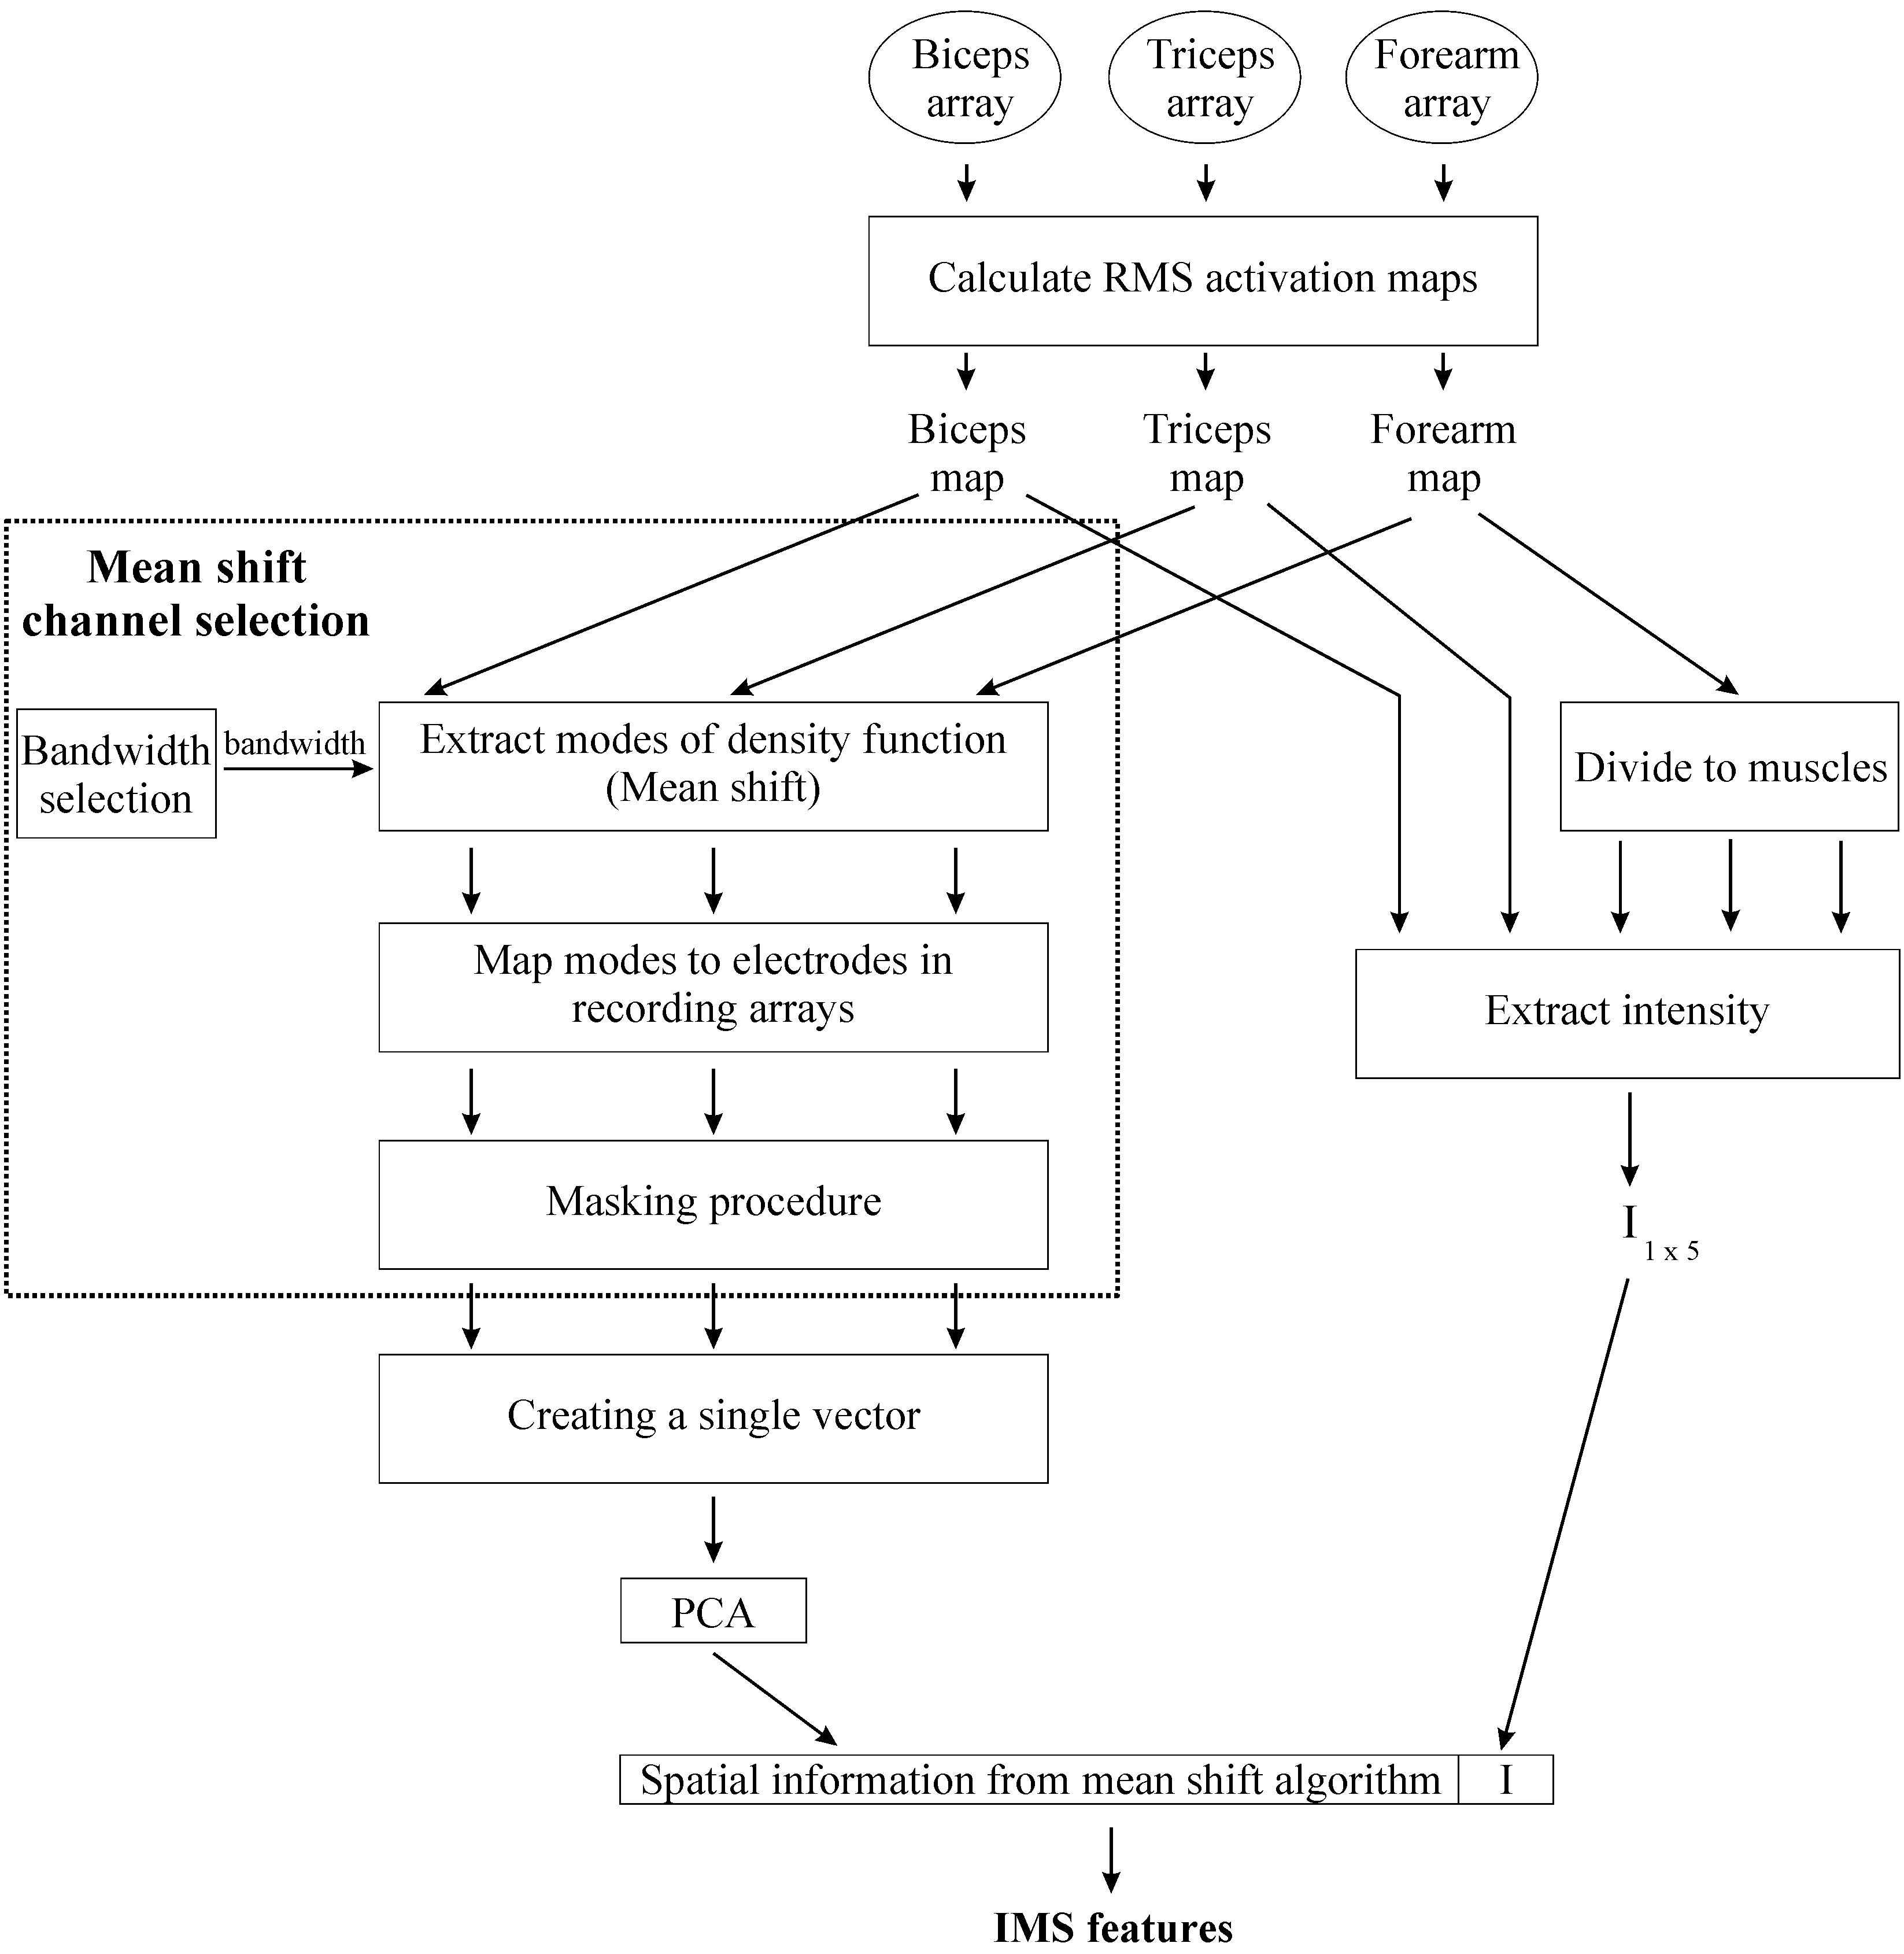
\includegraphics[width=0.9\textwidth]{Images/figure3_2.png}
\caption{Feature extraction flowchart.}
\label{fig:3-2}
\end{figure}   

The bandwidth $h$ was estimated automatically for each map. The maximum Euclidean distance between $k$ nearest neighbors (where $k$ was set to 50\% of the total number of elements in the map) was calculated for every sample and the average of the maximum distances was calculated. The bandwidth used in this paper was obtained by multiplying this average distance by a bandwidth factor of 0.5, selected as a tradeoff between the amount of information and the processing time.

Prior to using the mean shift algorithm, each RMS activation map was transformed to a matrix of $n$ rows, each row a channel, by three columns where the first two corresponded to the $x$, and $y$ location of the channel in the activation map and the third to its intensity as estimated from the RMS of the signal. Since we used the spherical kernel, i.e., the bandwidth $h$ had an equal value in all three dimensions, data was standardized to have zero mean and unity variance in all three dimensions.

A matrix of zeros with the same dimension of the electrode array was then created. Each mode detected by the mean shift algorithm was mapped to the closest location of the electrode in the array and its value was set to one. The result of this step was a binary image where the number of nonzero elements was equal to the number of detected modes. The procedure was repeated for all three activation maps. The resulting matrices were reshaped as a single $1-d$ vector in which the number of elements equaled to the total number of recorded EMG channels (for all three electrode arrays).

Principal component analysis (PCA) was then used for reducing the dimensionality of the feature space. A cumulative percentage of variance of 90\% was used for dimensionality reduction, i.e., after the transformation to the orthonormal space, features were ordered by variance, and only the features explaining at least 90\% of the cumulative variance were kept \citep{Valle1999}. This reduced spatial feature set was then combined with the intensity features.

For calculation of intensity features, HD-EMG activation maps were segmented into areas covering the targeted muscle following the same procedure described in \citep{Rojas-Martinez2012} and repeated in \citep{Rojas-Martinez2013}. Segmentation discards the map areas not covering the recorded muscle (e.g., edges of maps), and also divides the forearm map into three different maps which correspond to forearm muscles. From the resulting five segmented activation maps (biceps brachii, triceps brachii, brachioradialis, anconeus, and pronator teres), intensity features (I) were calculated as:

\begin{equation} \label{eq:3-3}
I = \log_{10} \frac{1}{N} \displaystyle\sum_{i,j} SAM_{i,j}
\end{equation}

where $I$ is the intensity feature, $SAM_{i,j}$ is the intensity value of the pixel at location $(i,j)$ in the segmented activation map $SAM$, and $N$ is the total number of pixels in that map. Therefore, this procedure extracts five intensity features, one for each muscle. By concatenation, these intensity features were combined with the reduced spatial features into a single feature vector. These generated features were used in the identification and will be referred to as IMS from now on.
Results were compared with the previously proposed feature set: a combination of intensity and center of gravity (ICG) of segmented activation maps \citep{Jordanic2016a, Jordanic2016b, Rojas-Martinez2013}. In this feature set, the center of gravity represents the traditional approach of describing the spatial information of intensity distribution over the muscle. The center of gravity ($CG$) has two dimensions and was calculated for each of the five muscles as:

\begin{equation} \label{eq:3-4}
CG = \frac{\displaystyle\sum_{i,j} SAM_{i,j} 
	\begin{bmatrix}
	  \, i \,\\
	  \, j \,\\
	\end{bmatrix}
	}{\displaystyle\sum_{i,j} SAM_{i,j}}
\end{equation}

Therefore, ICG is a feature vector of 15 dimensions. Identification was also performed using only intensity features (I), and two classical features, single differential signal (Diff) and time-domain features (TD). One differential signal was obtained from each of five muscles using a pair of electrodes selected within the electrode arrays. Two adjacent electrodes located over the location proposed by the SENIAM were used to obtain the differential signal. Feature used in the analysis is RMS value of the differential signal calculated over the 150 ms time window. On the other hand, five TD features were calculated for each recorded channel. These features were firstly proposed by Hudgins \citep{Parker2006} and used many times in literature \citep{Hakonen2015}. They were: RMS value, mean absolute value, number of zero crossings, waveform length, and number of slope sign changes. To be reduced in number, obtained features were projected to the space of lower dimensionality using PCA. As for the calculation of MS, only projections explaining 90\% of variance were kept.


\subsection{Task identification}
LDA was used for the identification of motor tasks. Task identification was evaluated using the repeated holdout method ($N = 20$). Observations were randomly assigned to the training set and the test set (70\% to the training set) using stratified sampling. Both the PCA transformation function and the LDA discriminant function were calculated on the training set, and evaluated on the test set. Only the results of the test set are presented. Identification results were expressed in terms of sensitivity ($S$) and precision ($P$), defined as:

\begin{equation} \label{eq:3-5}
S = \frac{TP}{TP + FN}
\end{equation}

\begin{equation} \label{eq:3-6}
P = \frac{TP}{TP + FP}
\end{equation}

where $TP$ (true positive) is the number of samples that were correctly classified, $FN$ (false negative) is the number of samples belonging to a certain class and erroneously classified into another class, whereas $FP$ (false positive) is the number of samples incorrectly classified to a certain class \citep{Sokolova2009}.

The identification was evaluated under various conditions:

\begin{itemize}
\item Short-term identification
\item Long term identification
\item Identification during fatigue
\end{itemize}

In short term identification, the training and validation sets were recorded at the same time. This are in fact the “perfect conditions” where the slow time-dependent changes in the sEMG signal associated with the recordings were minor. The dataset was composed of the recordings obtained in the first part of the measurement protocol.
Two types of identification were tested: identification of task and identification of task and effort level. In the identification of task, only the task was identified, regardless of the effort level, i.e., recordings of different effort levels were pooled together to form a single class. In this experiment, there were only four classes: flexion, extension, supination, and pronation. Identification of task and effort level was designed as a two-step classifier. In the first step the task was identified, regardless of the effort level, as discussed above. In the second step, classification of three levels of effort was performed for each identified task individually. The second step consisted of four different classifiers, one classifier for the identification of the effort level of each task. For identification of effort level of a sample, the second step classifier was selected depending on the classified task in the first step \citep{Jordanic2016b}. Classifiers in the second step were designed using the reduced feature set, as proposed in \citep{Jordanic2016b}, where features were extracted from agonist-antagonist muscle pairs involved in the selected task, i.e., biceps brachii and triceps brachii for identification of the effort level during flexion and extension; biceps brachii, brachioradialis and anconeus for supination; and pronator teres and anconeus for pronation. Since the modes of the density function were calculated for the entire forearm array (not for each muscle separately), modes extracted from the entire forearm array were used in the identification of the effort level during supination and pronation.
In the long-term identification, robustness to time effect was tested. In this part of the protocol, the training set was composed of all observations recorded in the first part of the measurement protocol, whereas the test set was composed of the first two seconds of the recordings in the second part of the protocol. Having in mind that there was a time gap between the first part of the protocol and the second part of the protocol ($\approx$30 min), using this procedure the influence of different time effects can be evaluated (e.g., drying of conductive gel). On the other hand, to prevent the effect of fatigue, only the first two seconds of the total duration of the exercise were used in the test set.
Robustness of the identification was also tested during endurance tasks recorded during the second part of the recording protocol. Recordings were divided into five equal time epochs. The classifier was trained using the samples extracted from the first 20\% of the total duration of recording (TDR), and was evaluated on five equally long segments throughout the exercise: 0–20\% TDR, 20–40\% TDR, 40–60\% TDR, 60–80\% TDR, and 80–100\% TDR.


\subsection{Statistical methods}
Statistical difference in performance was checked between IMS and other feature sets. The Kolmogorov-Smirnov test showed that the data significantly deviate from a normal distribution, so the non-parametric statistical Wilcoxon signed rank test was used to test for differences between distributions. In addition, the non-parametric repeated measures Friedman test was used to test the differences in identification of the task when the training set was composed of pool of all effort levels, and test set of only 10\% MVC, 30\% MVC, or 50\% MVC. This was repeated for all feature sets. The significance level was set to $p = 0.05$. Statistical tests were performed using the IBM SPSS Statistics software package (IBM SPSS Statistics for Windows, version 20.0, released 2011; IBM Corp.: Armonk, NY, USA).
\clearpage


\section{Results} \label{sc:3-3}
\subsection{Bandwidth and time window selection}
Two aspects where considered in the choice of the bandwidth factor: the average execution time of the mean shift algorithm and the amount of information, i.e., number of detected modes (Figure \ref{fig:3-3}). The average processing time was measured on a standard desktop computer featuring an Intel\textregistered \, E8400 Core\textsuperscript{TM} 2 Duo CPU (Intel, Santa Clara, CA, USA). Both graphs show that the elbow point was at the bandwidth factor of 0.5. If the bandwidth factor is set to a lower value, both the execution time and the number of modes increase notably. A rapid increase of the number of modes for lower bandwidths implies that the mean shift algorithm is focused on local maxima, whereas the increase of the execution time increases the latency of the system. On the other hand, there was not much difference when the bandwidth factor ranges between 0.5 and 1.0, both in the number of estimated modes, and the execution time. Therefore, the range from 0.5 to 1.0 was considered of interest for the selection of the bandwidth factor.

\begin{figure}[ht]
\centering
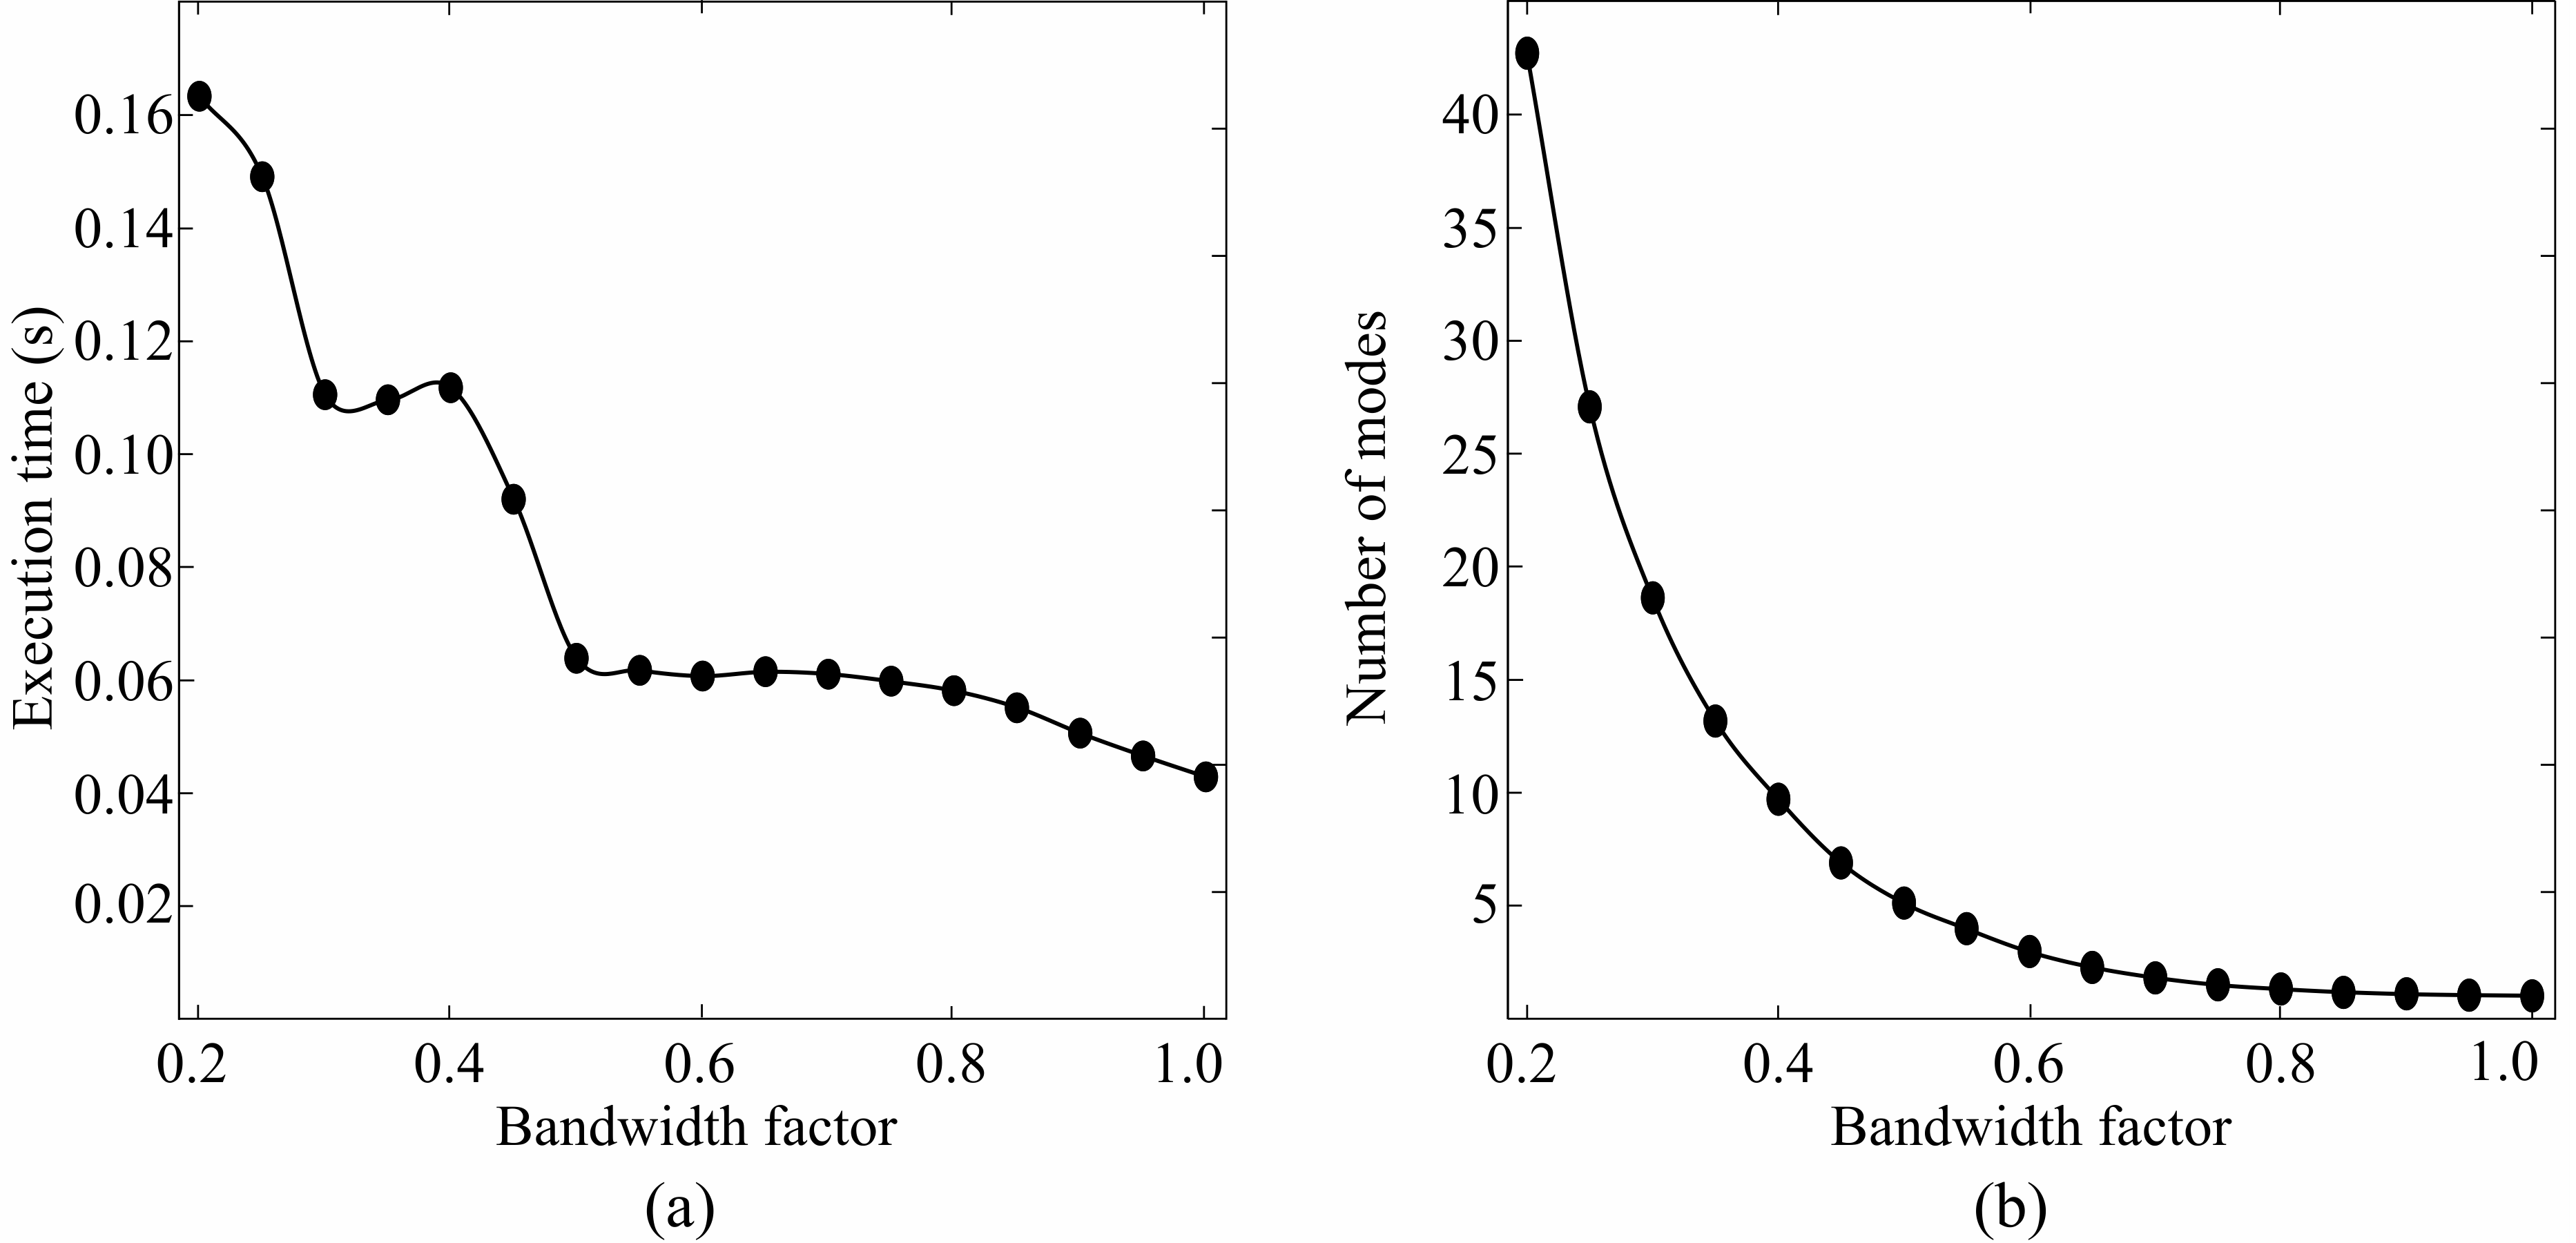
\includegraphics[width=0.9\textwidth]{Images/figure3_3.png}
\caption{Figure shows average processing time (a) and number of estimated modes (b) of mean shift algorithm given the specific bandwidth factor in the range from 0.2 to 1.}
\label{fig:3-3}
\end{figure}   

The identification of task and the identification of task and effort level (Figure \ref{fig:3-4}) were compared using the bandwidth factor of 0.5 and 1.0. The performance of the algorithm was significantly higher when using the bandwidth of 0.5 compared with that of 1 ($p < 0.05$).

\begin{figure}[ht]
\centering
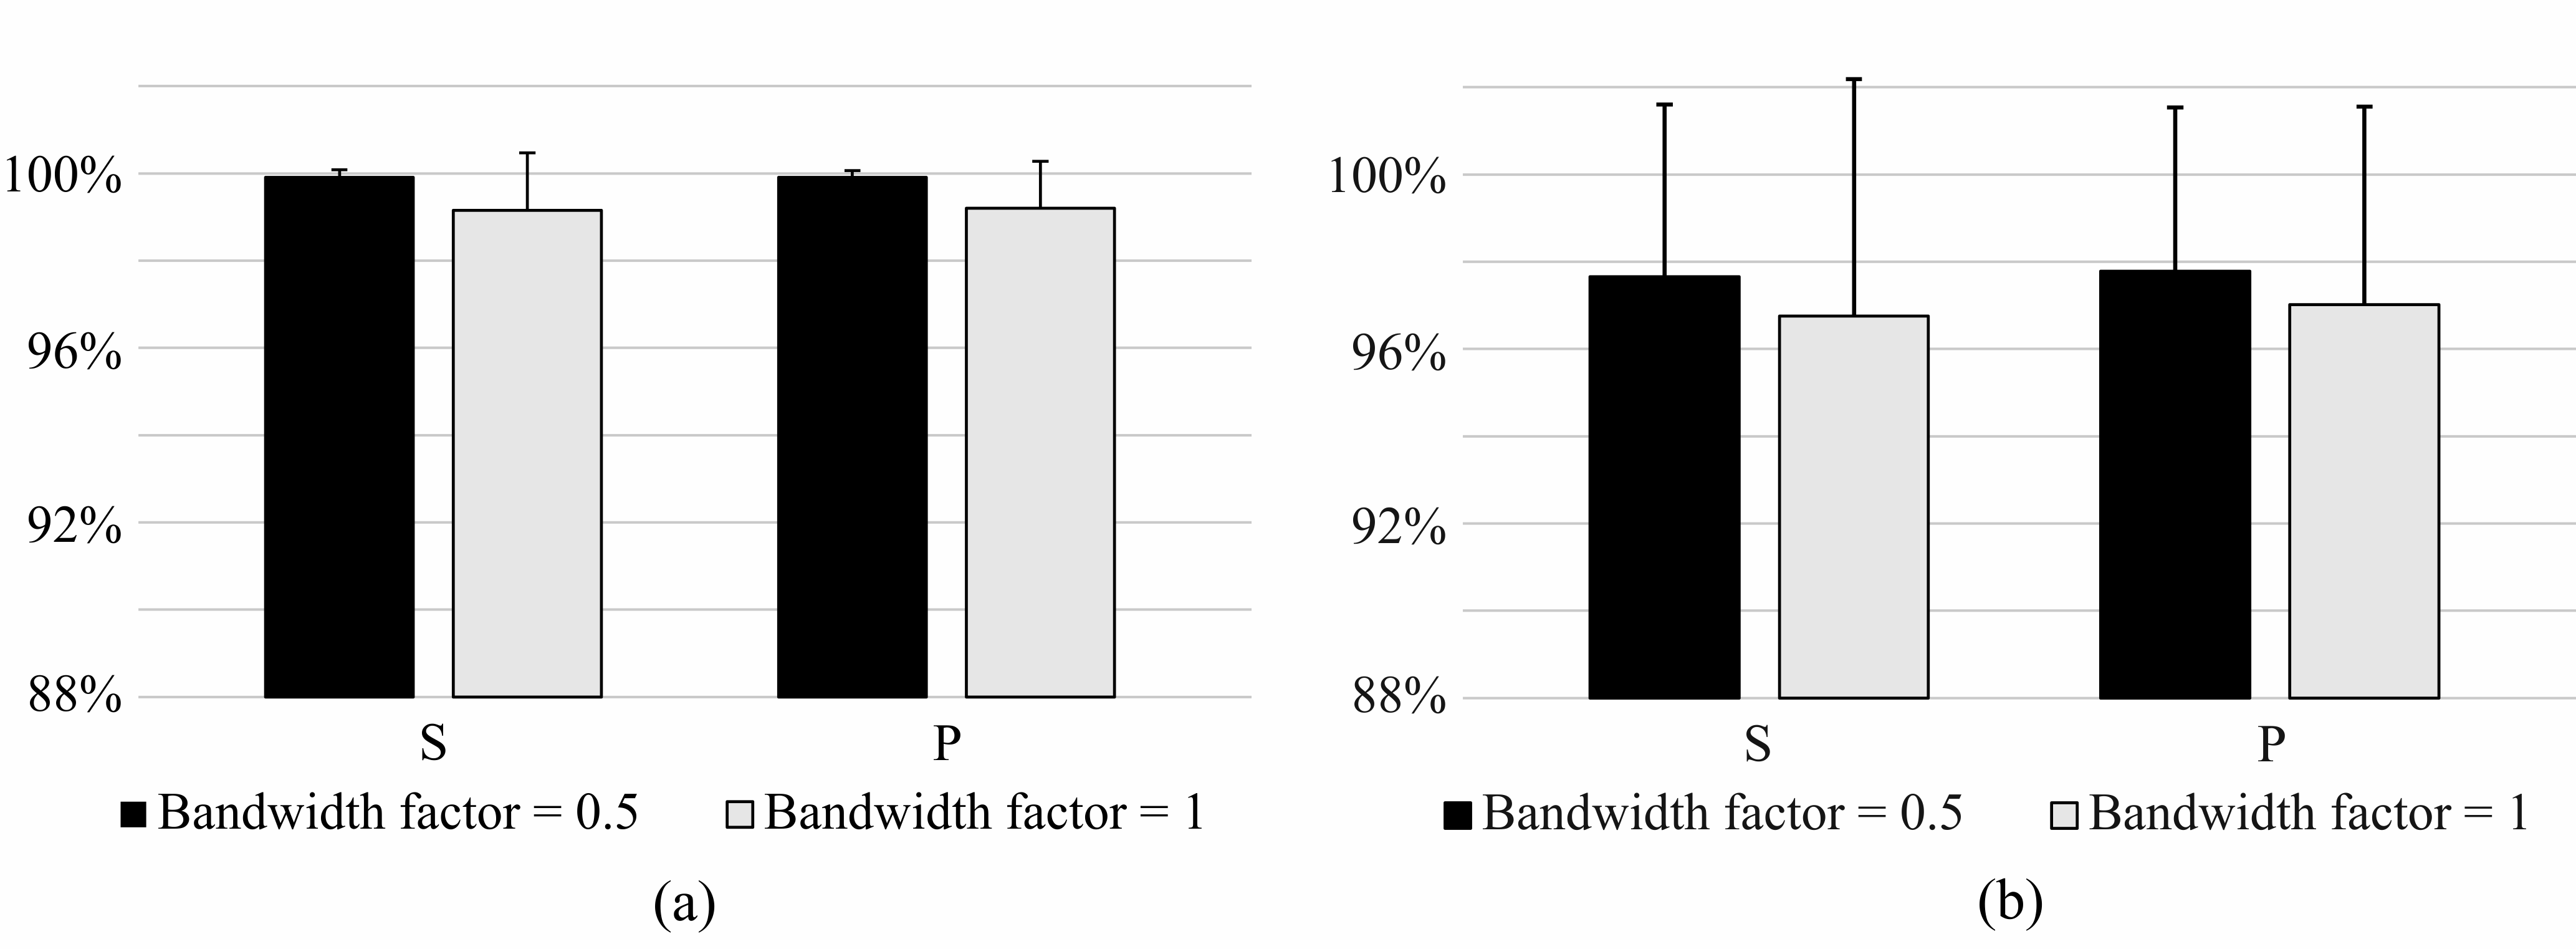
\includegraphics[width=0.9\textwidth]{Images/figure3_4.png}
\caption{Sensitivity and precision of short-term identification of (a) identification of task and (b) identification of task and effort level using bandwidth factors 0.5 and 1.0 in mean shift algorithm.}
\label{fig:3-4}
\end{figure}   

On the other hand, the effect of duration of time window in which the features were calculated was analyzed and results are presented in Figure \ref{fig:3-5}. Identification based on the IMS features extracted from the 150 ms and 200 ms time windows significantly outperform the identification when features were extracted from shorter time windows, whereas no significant difference was found between results calculated on 150 ms and 200 ms windows.

\begin{figure}[ht]
\centering
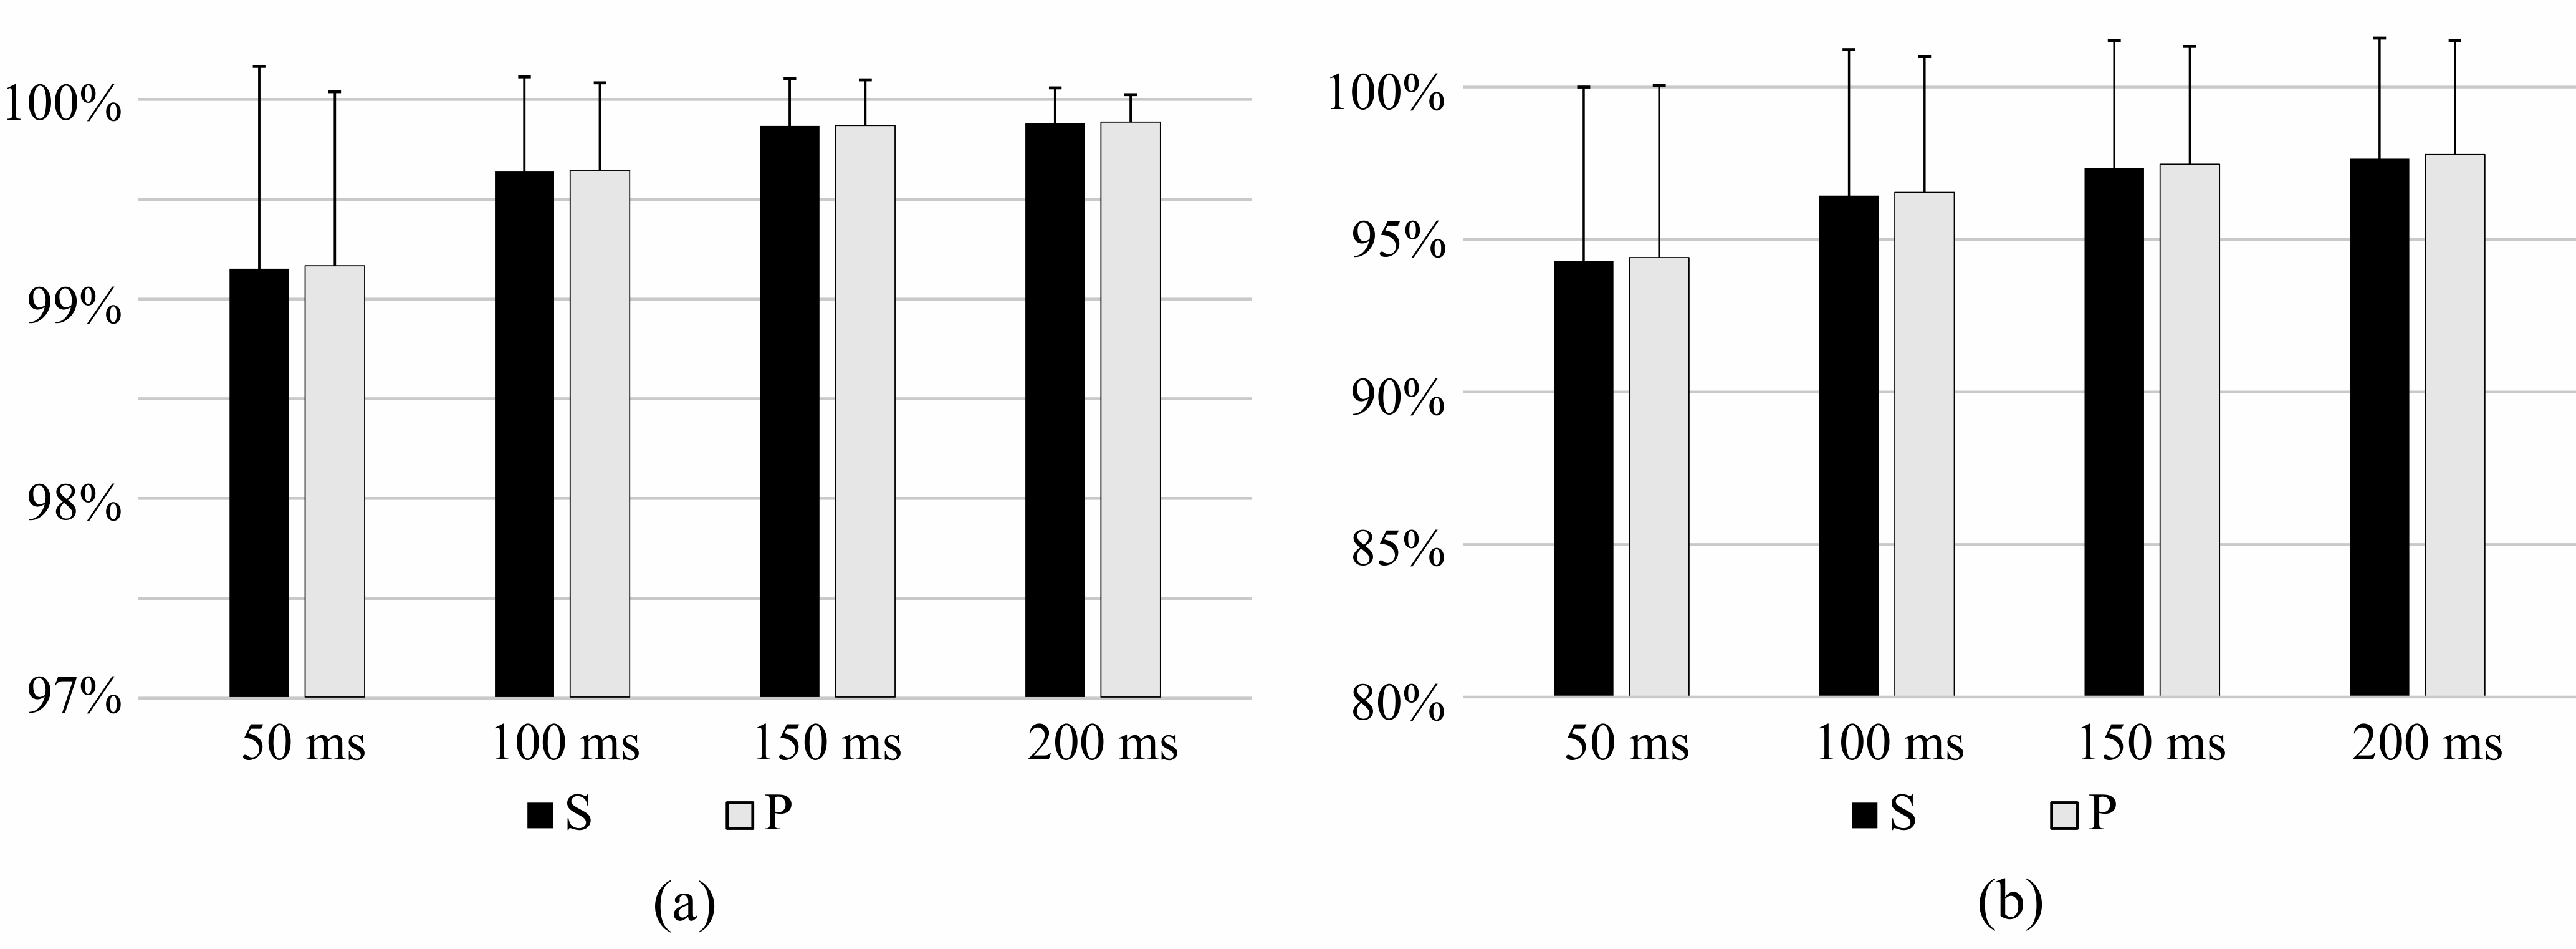
\includegraphics[width=0.9\textwidth]{Images/figure3_5.png}
\caption{Sensitivity (S) and precision (P) of (a) identification of task and (b) identification of task and effort level for time windows of 50 ms, 100 ms, 150 ms, and 200 ms.}
\label{fig:3-5}
\end{figure}   

Consequently, the bandwidth factor of 0.5 and the time window of 150 ms were used in the rest of the paper.

\subsection{Short-term identification}
Table \ref{tb:3-1} shows the results of the identification of task using the novel features proposed in this paper and Figure \ref{fig:3-6} shows the comparison between IMS, ICG, I, TD, an Diff features in the identification of tasks. IMS significantly outperformed all of the compared features ($p < 0.05$).

\begin{figure}[ht]
\centering
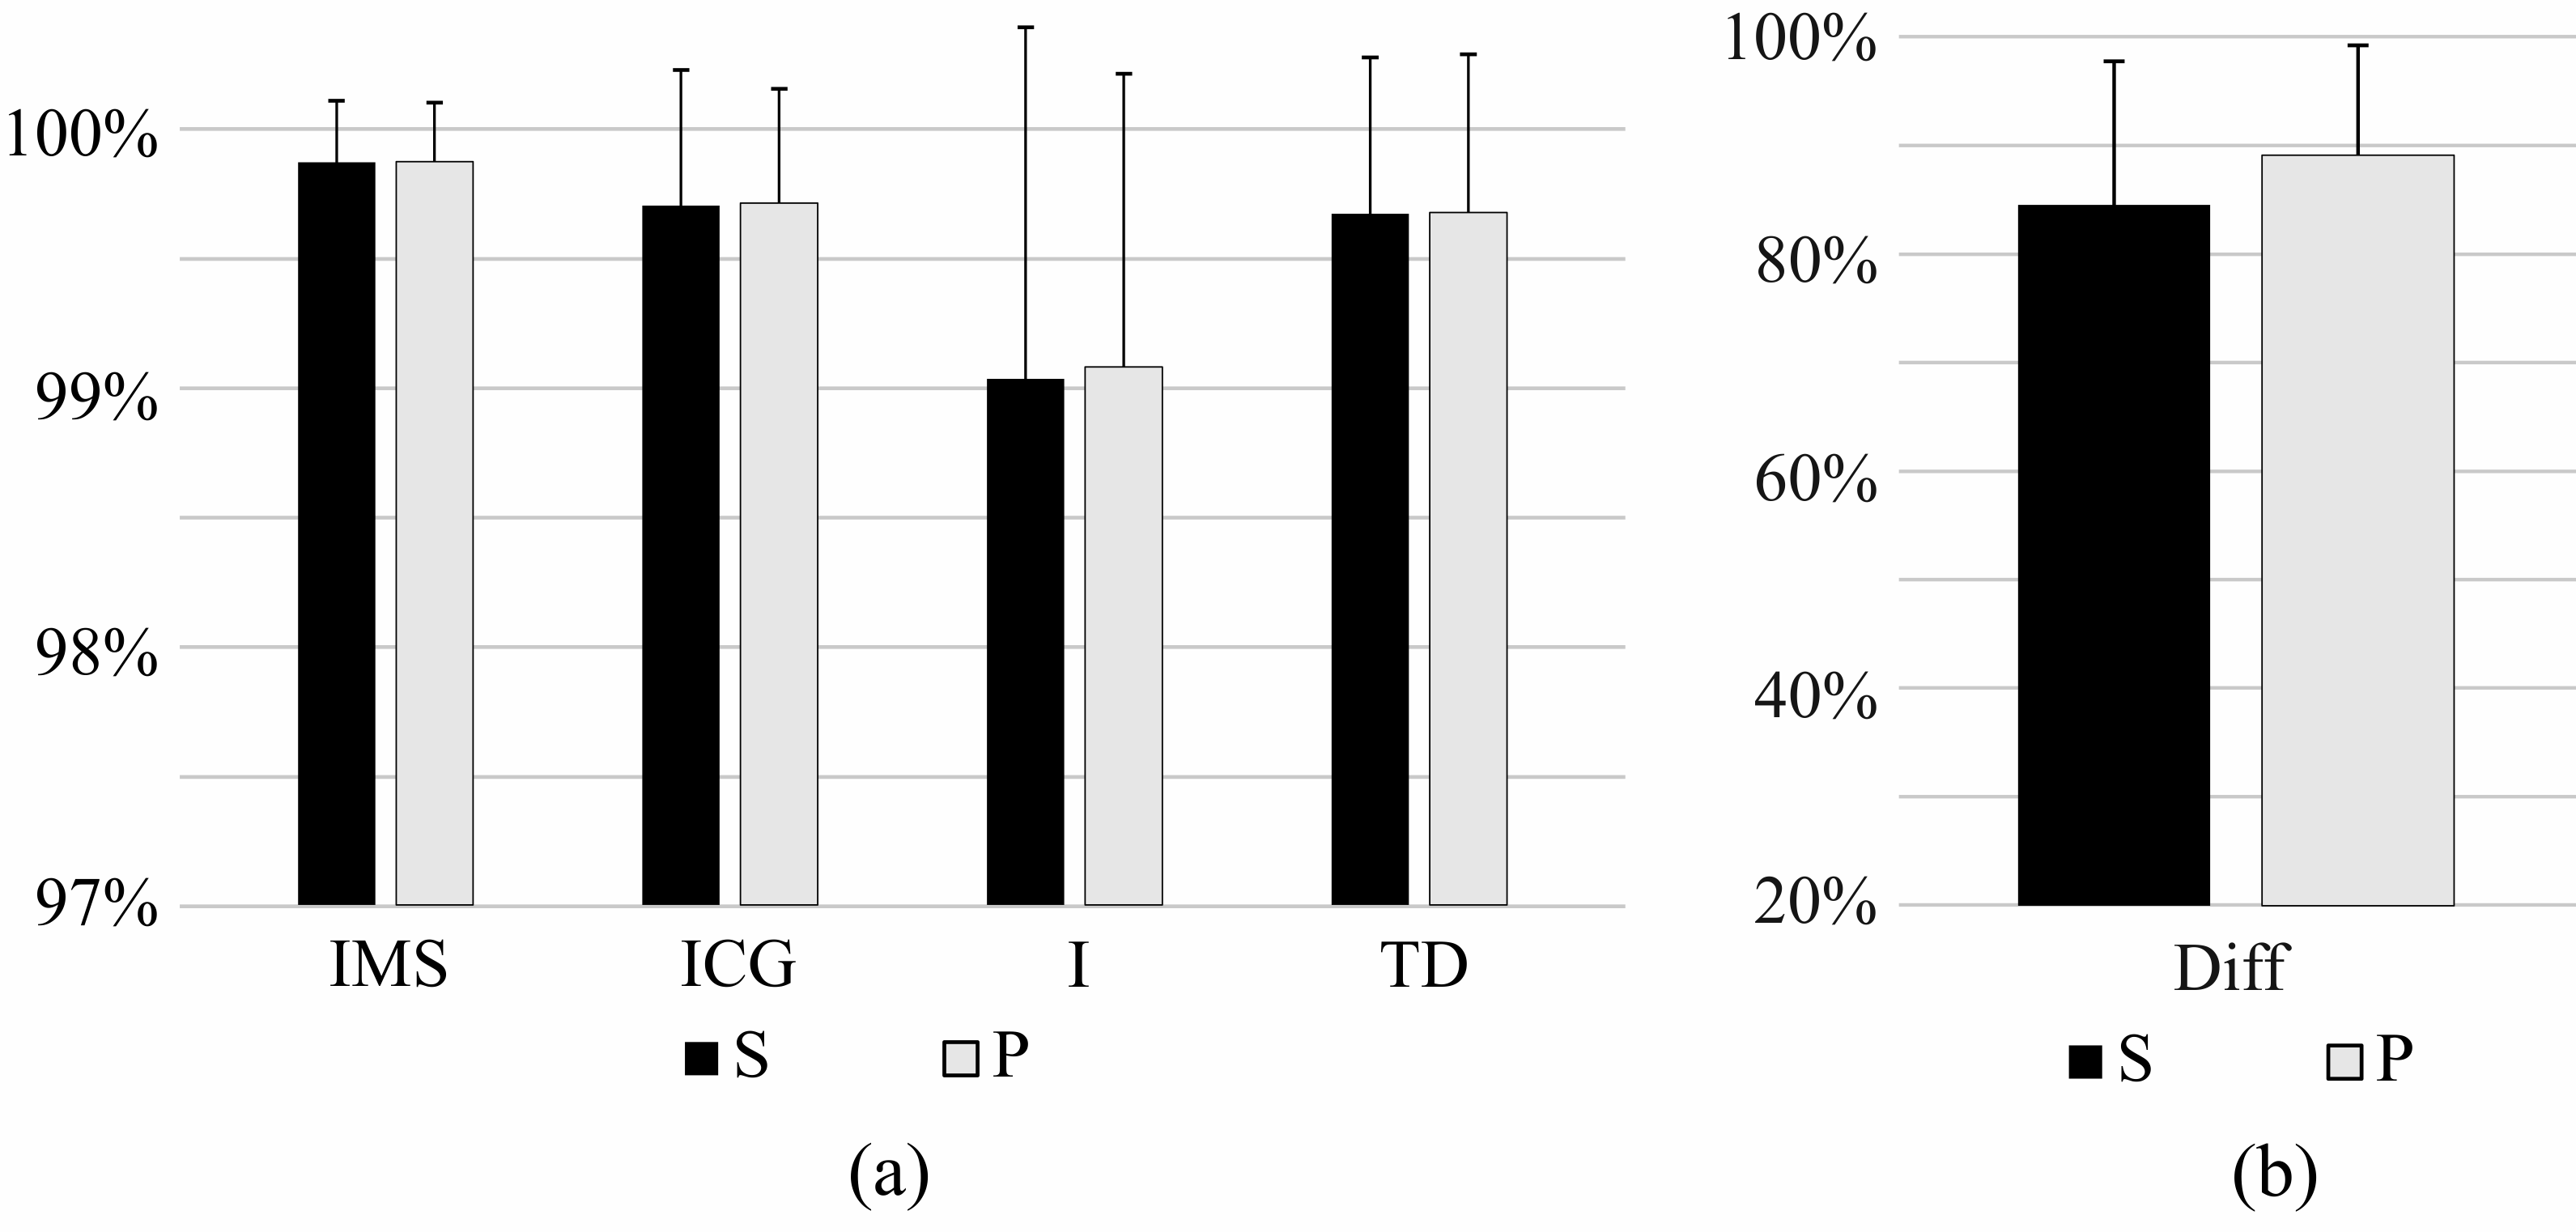
\includegraphics[width=0.9\textwidth]{Images/figure3_6.png}
\caption{Sensitivity (S) and precision (P) of short-term identification of task using (a) IMS, ICG, I, and TD features, and (b) using Diff features. Results of the identification using Diff is showed in a different scale.}
\label{fig:3-6}
\end{figure}   

\begin{table}[h!]
\centering
\caption{Sensitivity and precision of identification of task using IMS features averaged between patients. Identification Indices for each patient were calculated as an average of hold-out repetitions ($N = 20$) and presented in terms of mean and standard deviation.}
\small
\vspace{3mm}
\label{tb:3-1}
\begin{threeparttable}
\begin{tabular}{lcc}
Task       & Sensitivity\%           & Precision \% \\ \hline
              &                &                                              \\
Flexion             & 99.7 $\pm$ 0.5             & 99.9 $\pm$ 0.2                      \\
Extension             & 99.9 $\pm$ 0.1             & 99.9 $\pm$ 0.1                      \\
Supination             & 99.9 $\pm$ 0.2             & 99.7 $\pm$ 0.5                          \\
Pronation             & 99.9 $\pm$ 0.1            & 99.9 $\pm$ 0.1             \\
\textbf{Average}             & \textbf{99.9 $\pm$ 0.2}             & \textbf{99.9 $\pm$ 0.2}           
\end{tabular}
    \end{threeparttable}
\end{table}


The results of the identification of the task and effort level using IMS features are given in Table \ref{tb:3-2}, whereas comparison between IMS and other features is shown in Figure \ref{fig:3-7}. IMS features significantly outperform I, TD, and Diff features ($p < 0.05$), whereas the ICG features slightly outperform IMS features ($\Delta$S = 0.6\%, $\Delta$P = 0.6\%; $p < 0.05$).

\begin{figure}[ht]
\centering
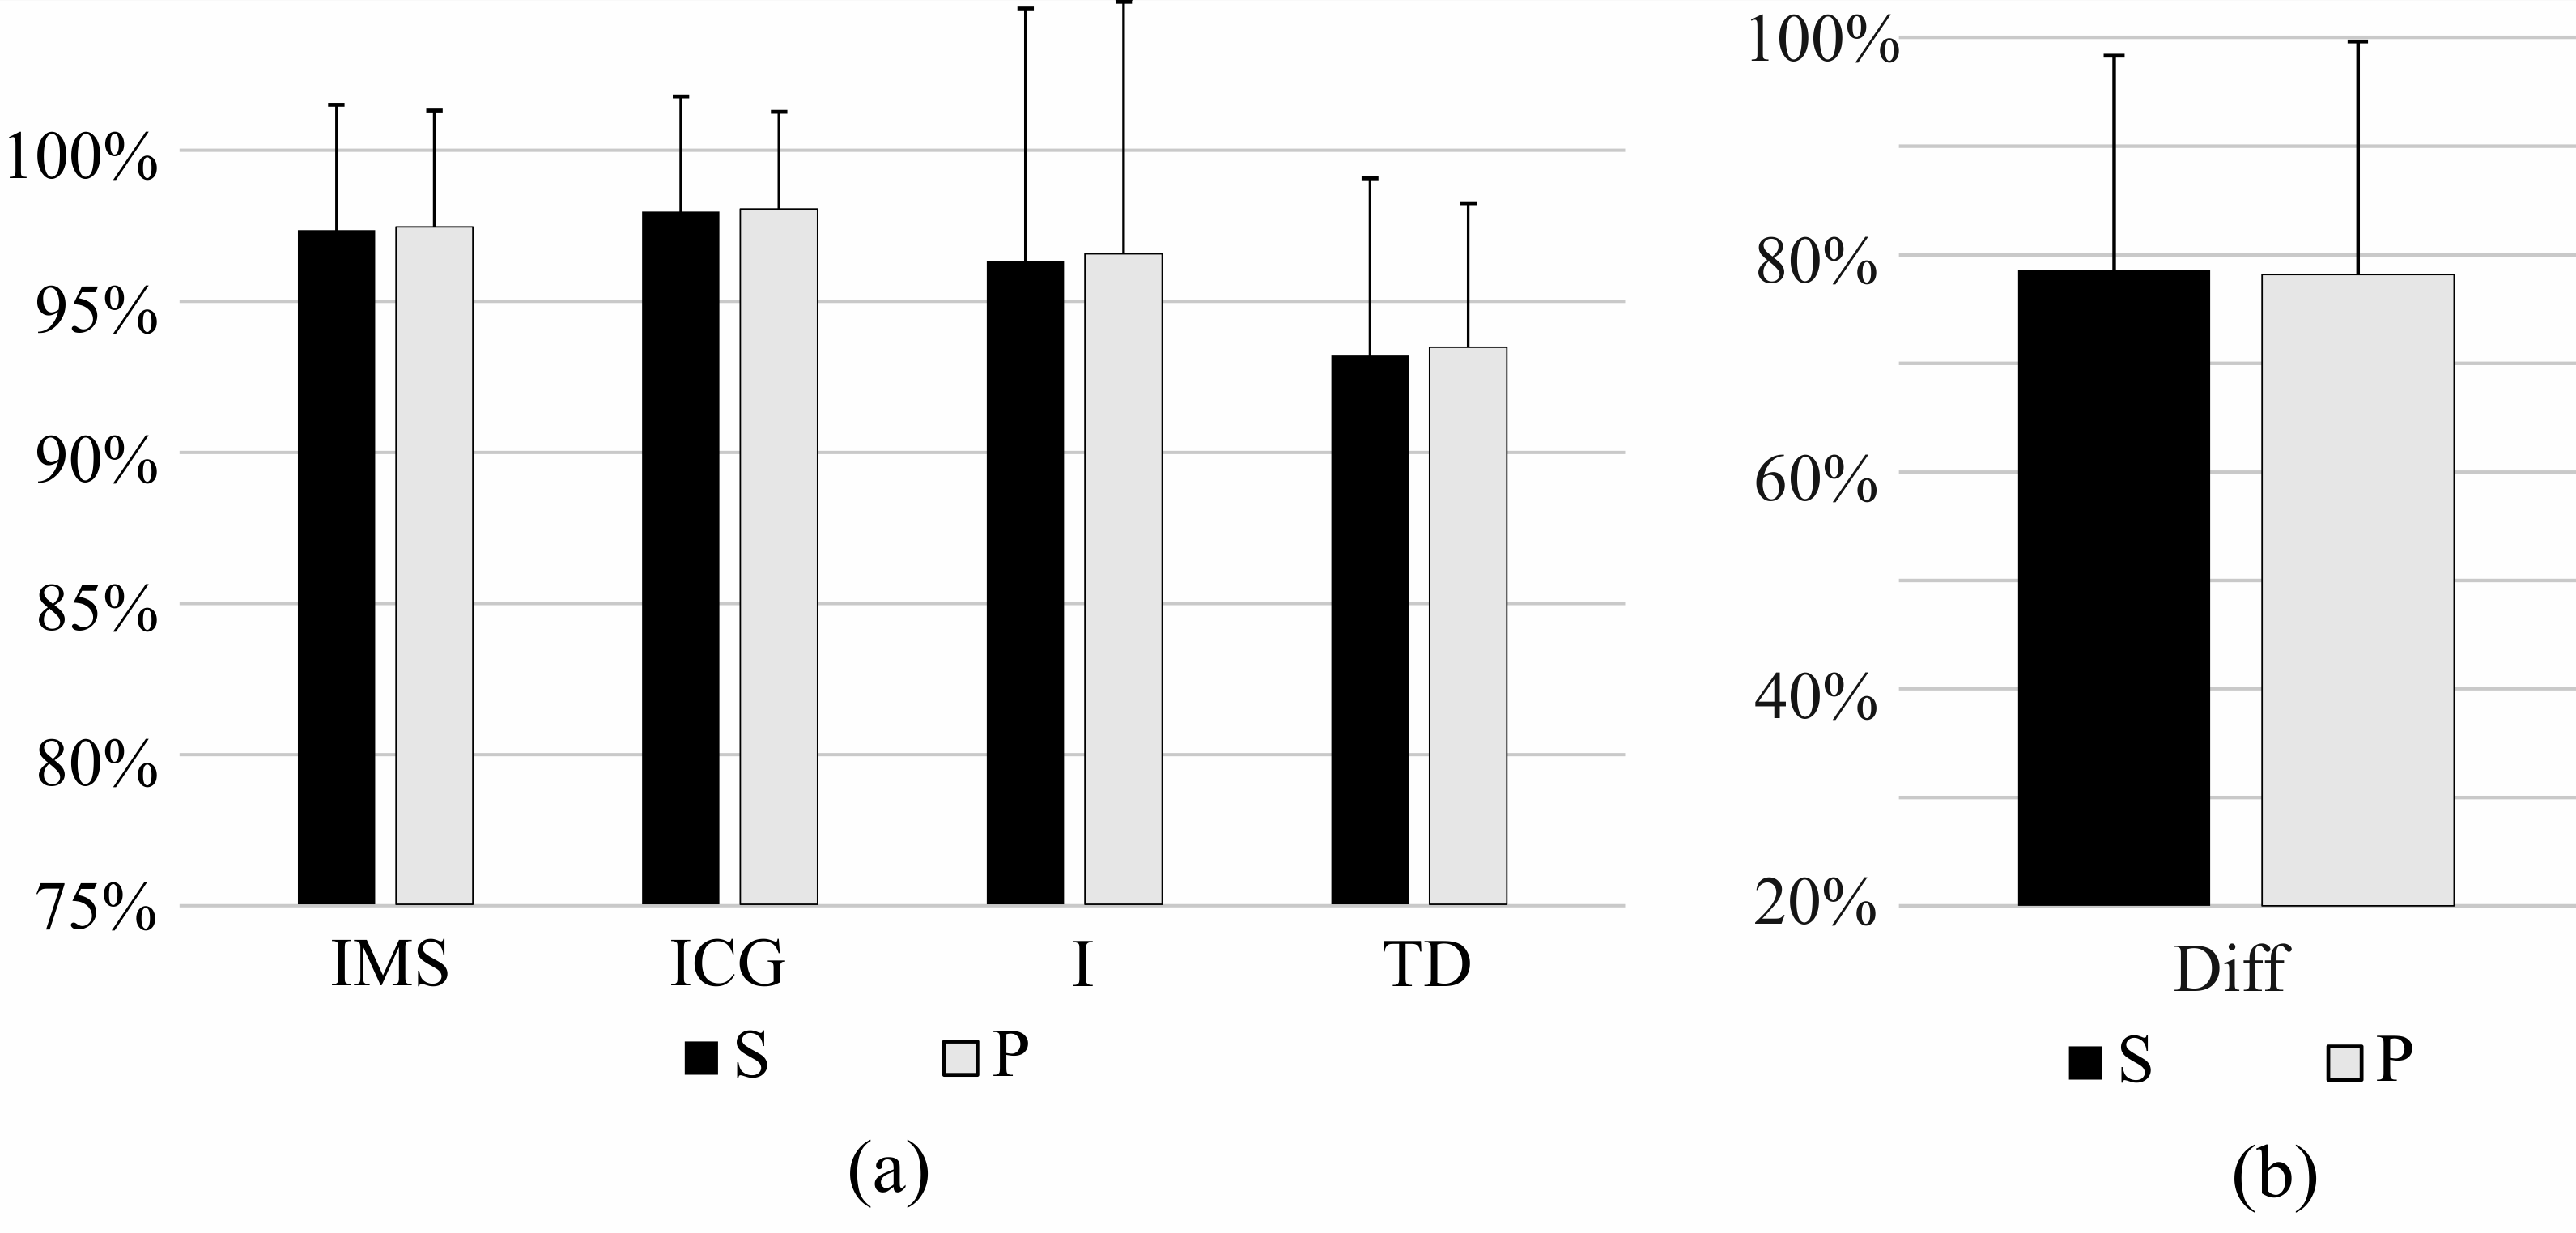
\includegraphics[width=0.9\textwidth]{Images/figure3_7.png}
\caption{Sensitivity (S) and precision (P) of short-term identification of task and effort level using (a) IMS, ICG, I, and TD features, and (b) using Diff features. Results of the identification using Diff is showed in a different scale.}
\label{fig:3-7}
\end{figure}   

\begin{table}[h!]
\centering
\caption{Sensitivity and precision of identification of task and effort level averaged between patients. Identification indices for each patient were calculated as an average of hold-out repetitions (N = 20) and presented in terms of mean and standard deviation.}
\small
\vspace{3mm}
\label{tb:3-2}
\begin{threeparttable}
\begin{tabular}{lcc}
Task       & Sensitivity\%           & Precision \% \\ \hline
              &                &                                              \\
Flexion 10\% MVC             & 98.2 $\pm$ 2.8             & 99.9 $\pm$ 0.3                      \\
Flexion 30\% MVC             & 98.7 $\pm$ 1.1            & 97.0 $\pm$ 3.1                      \\
Flexion 50\% MVC             & 97.7 $\pm$ 2.9             & 98.6 $\pm$ 1.1                         \\
Extension 10\% MVC             & 99.7 $\pm$ 0.6            & 99.6 $\pm$ 1.1             \\
Extension 30\% MVC             & 97.4 $\pm$ 3.4             & 97.5 $\pm$ 2.1                      \\
Extension 50\% MVC             & 97.7 $\pm$ 2.3             & 98.2 $\pm$ 2.9                      \\
Supination 10\% MVC             & 99.7 $\pm$ 0.5             & 99.9 $\pm$ 0.2                          \\
Supination 30\% MVC             & 95.2 $\pm$ 7.1            & 96.0 $\pm$ 5.1             \\
Supination 50\% MVC             & 96.6 $\pm$ 4.9             & 95.4 $\pm$ 6.3                      \\
Pronation 10\% MVC             & 99.8 $\pm$ 0.2             & 99.4 $\pm$ 1.1                      \\
Pronation 30\% MVC             & 93.8 $\pm$ 12.3             & 93.9 $\pm$ 11.3                          \\
Pronation 50\% MVC             & 93.7 $\pm$ 11.9            & 94.2 $\pm$ 11.9             \\
\textbf{Average}             & \textbf{97.4 $\pm$ 4.2}             & \textbf{97.5 $\pm$ 3.9}           
\end{tabular}
    \end{threeparttable}
\end{table}


The sensitivity and precision of the task identification when the classifier was trained using all effort levels (pool of 10\%, 30\%, 50\% MVC) and tested using a specific effort level can be seen in Figure \ref{fig:3-8} and Figure \ref{fig:3-9} for comparison of IMS, ICG, I, and TD features, and for Diff features, respectively. This experiment shows how well each feature set identifies the task of a specific effort level. The difference in performance is especially pronounced in the identification of tasks at very low effort level (10\% MVC). IMS significantly outperforms I and Diff features at all effort levels, but the difference between IMS and ICG features and the difference between IMS and TD are not significant at moderate effort levels (30\% MVC and 50\% MVC), whereas IMS features are specifically and significantly better when identifying tasks at low effort levels (10\% MVC).

\begin{figure}[ht]
\centering
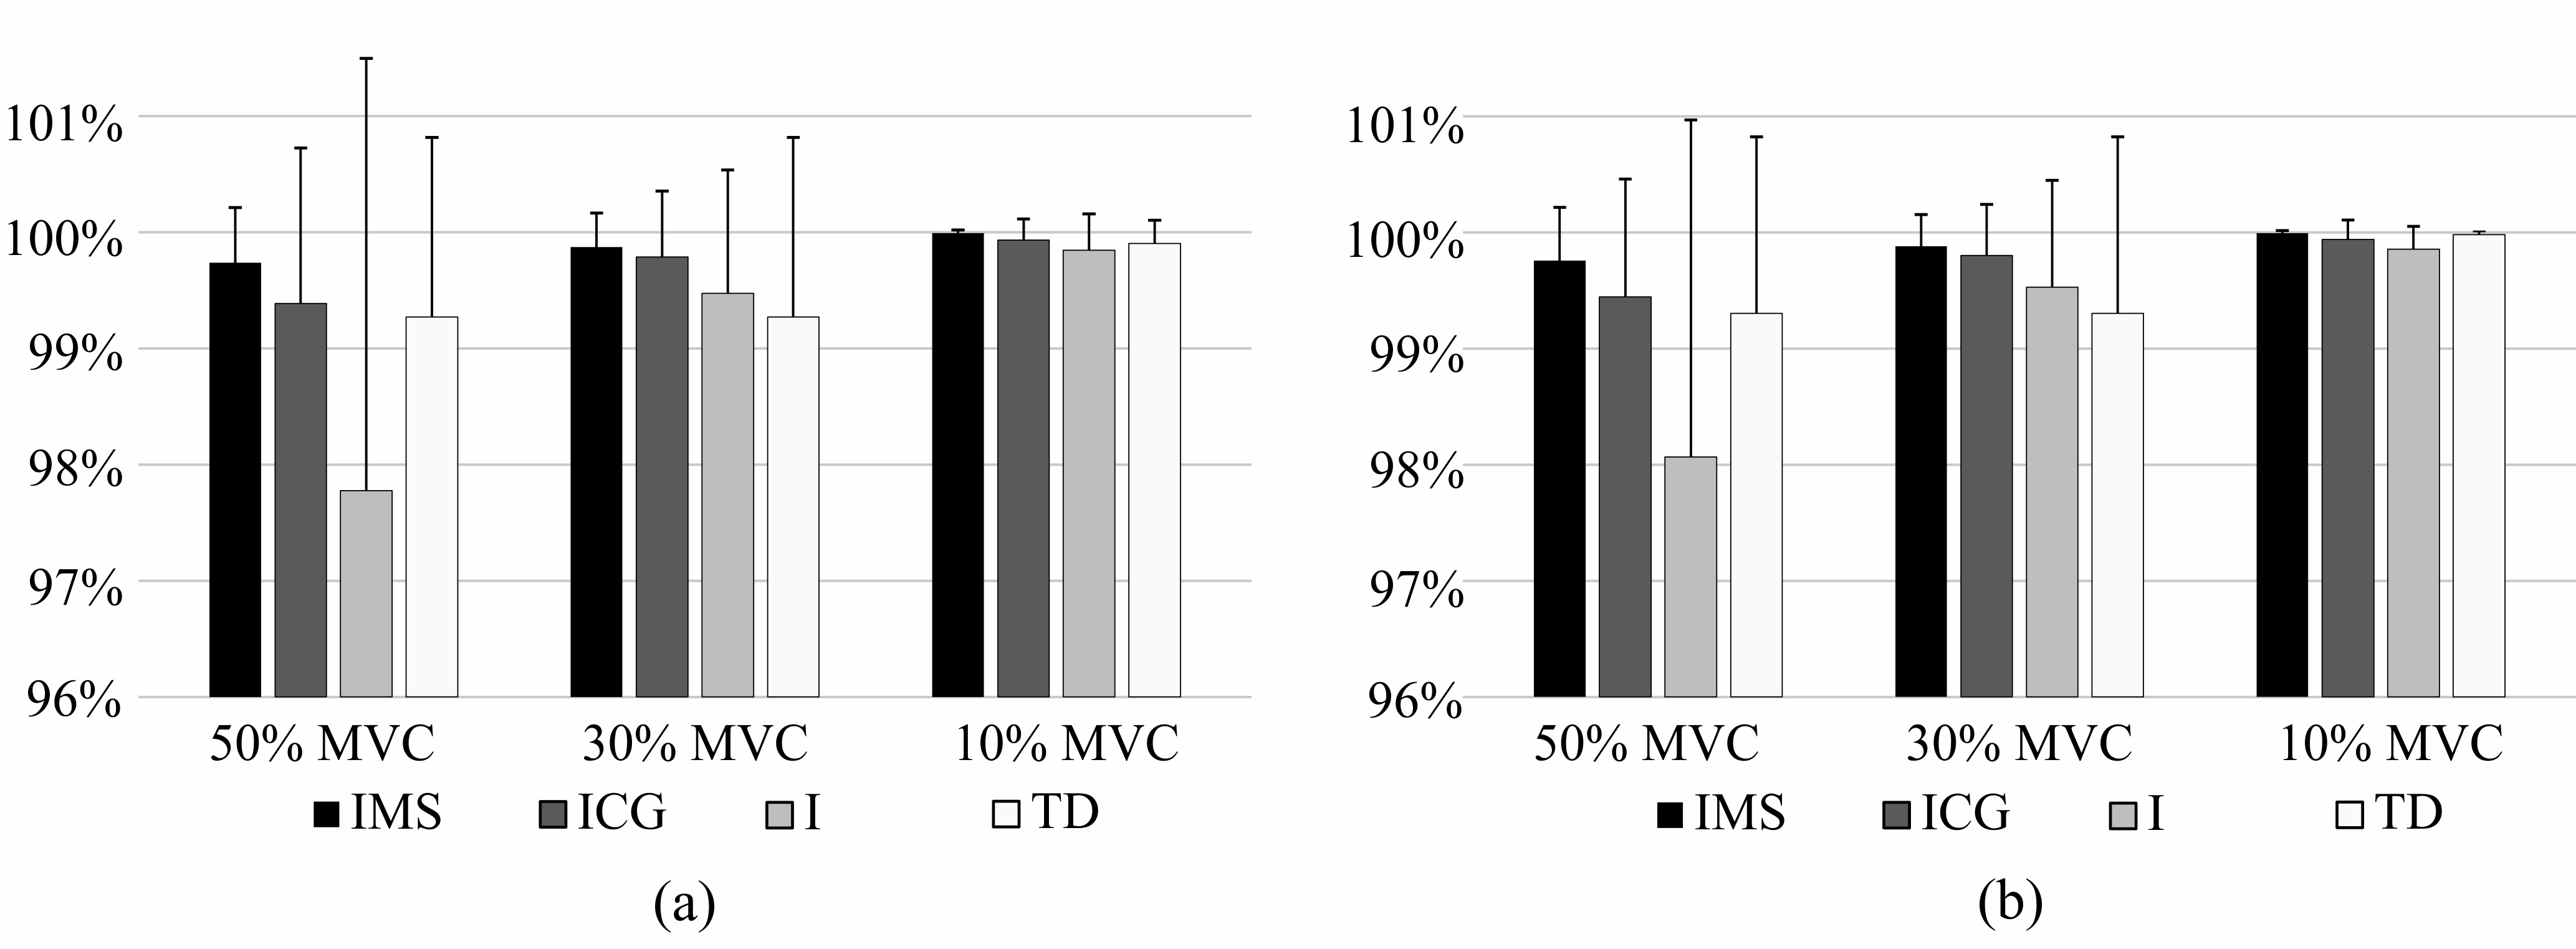
\includegraphics[width=0.99\textwidth]{Images/figure3_8.png}
\caption{Figure shows sensitivity (a) and precision (b) of short-term identification of task recorded at specific effort level using IMS, ICG, I, and TD features.}
\label{fig:3-8}
\end{figure}   

\begin{figure}[ht]
\centering
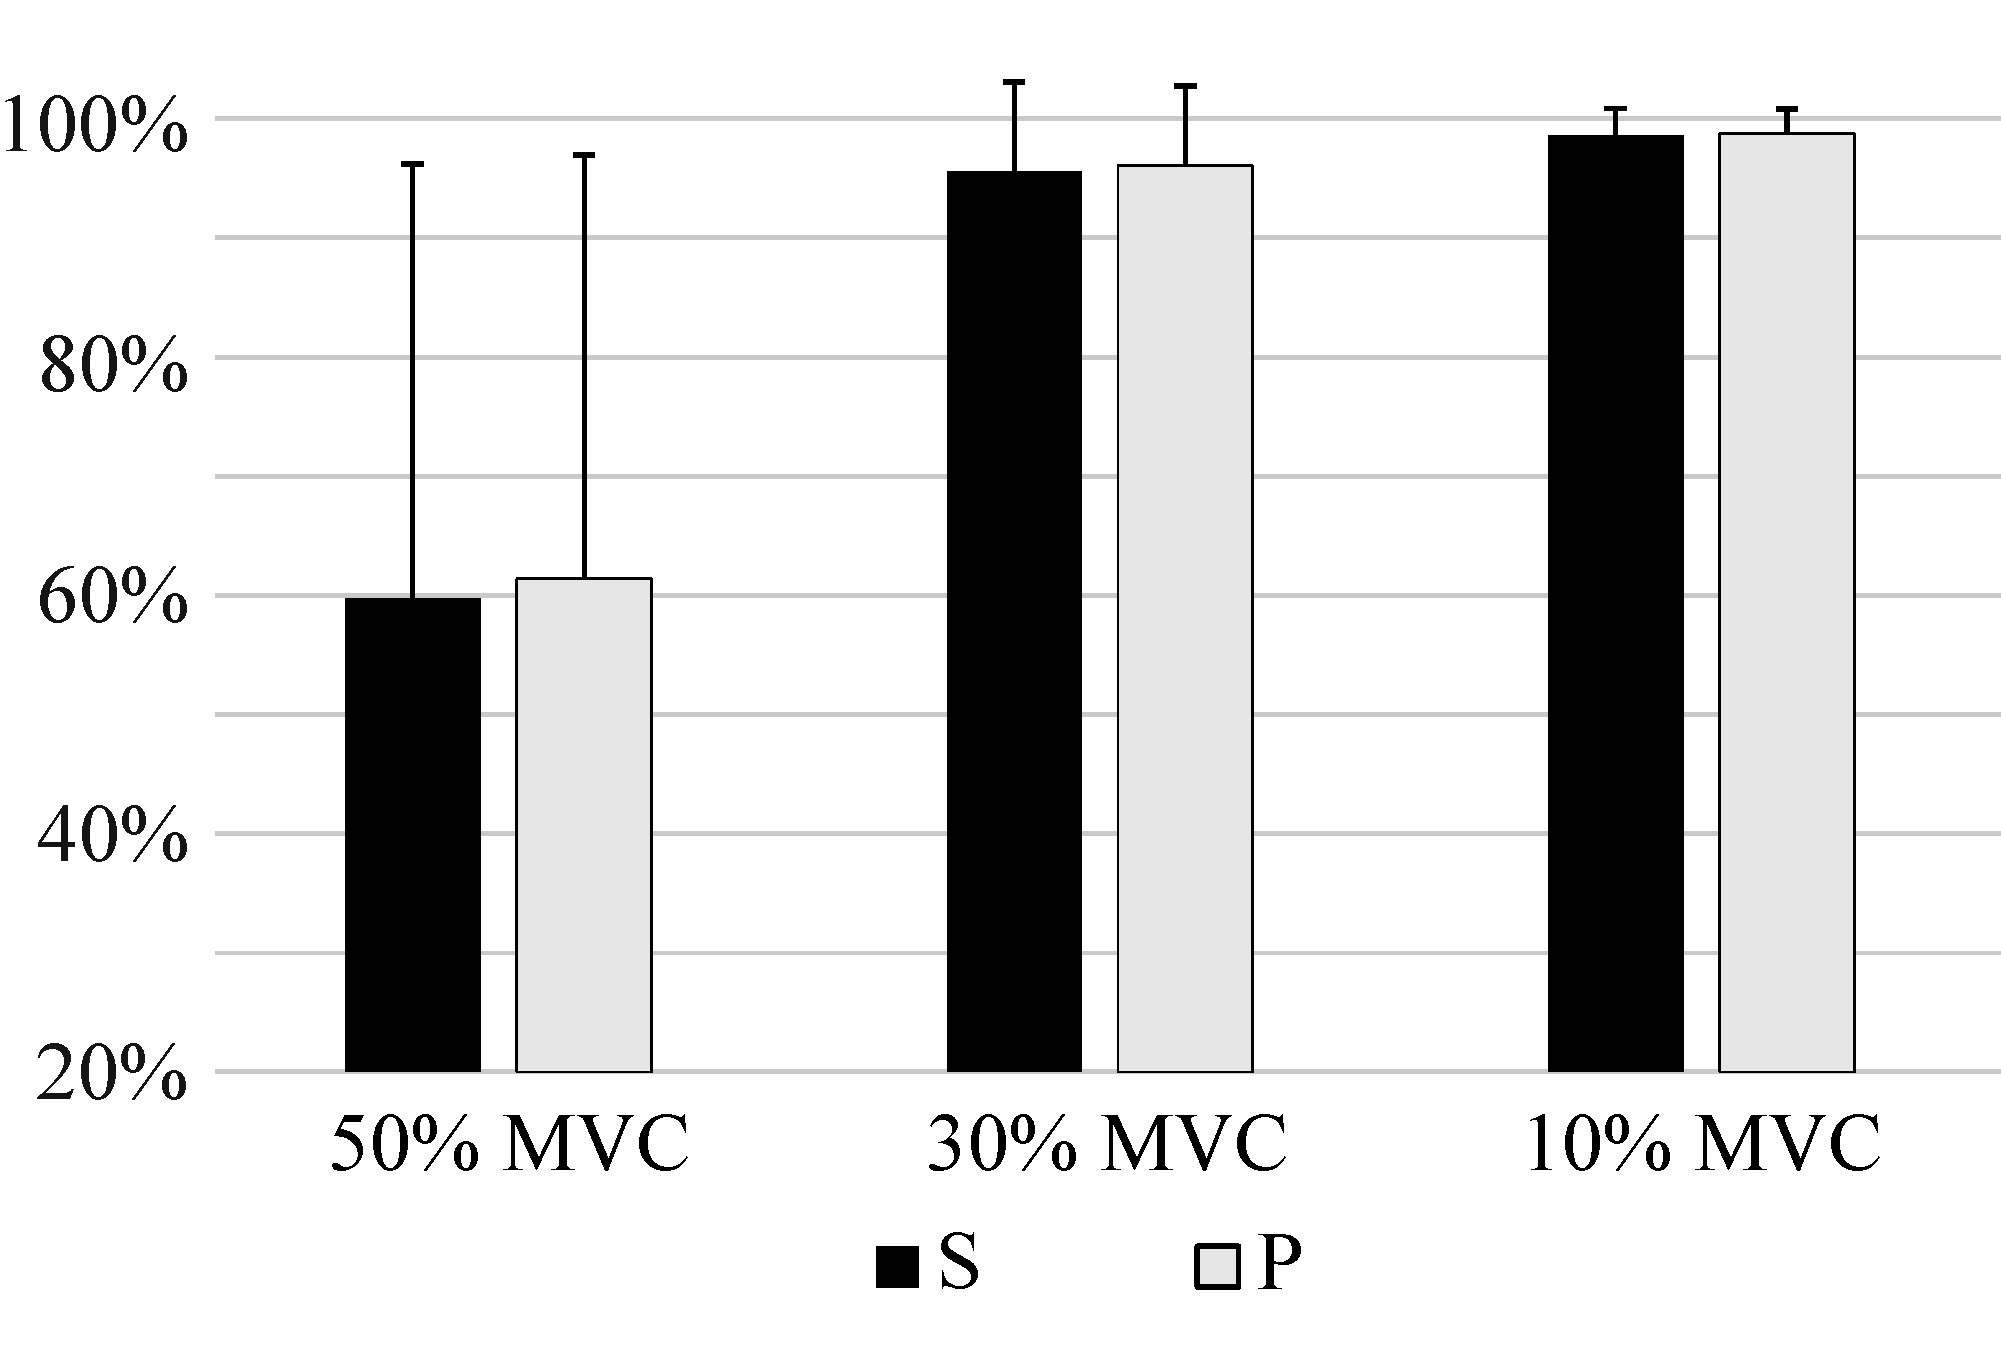
\includegraphics[width=0.45\textwidth]{Images/figure3_9.png}
\caption{Figure shows sensitivity (S) and precision (P) of short-term identification of task recorded at specific effort level using Diff features.}
\label{fig:3-9}
\end{figure}   

Additionally, no significant difference between task identification at three different effort levels was seen when using IMS features, whereas these differences were significant for other feature sets. This could mean that these novel IMS features are more robust to the variation in the effort level.

\subsection{Long-term identification}
Identification was tested when a significant amount of time passed between the recording of the training and test sets. This allowed an evaluation of influence of slow time-dependent changes in the EMG signal on the robustness of the identification. Figure \ref{fig:3-10} shows the comparison of the intensity features and the combination of intensity and spatial features when these last ones were calculated as the center of gravity or using the mean shift algorithm. There are no significant differences in performances between these IMS, ICG, and I features, whereas IMS feature significantly outperform TD and Diff features ($p < 0.05$). However, it should be noted that the test set was composed only of samples recorded at 50\% MVC. And, as previously proven in literature \citep{Jordanic2016a}, and shown in Figure \ref{fig:3-8} and Figure \ref{fig:3-9}, the use of spatial information is particularly useful in contractions at low effort levels, whereas only intensity can be sufficient to successfully identify contractions of moderate effort levels (as 50\% MVC).

\begin{figure}[ht]
\centering
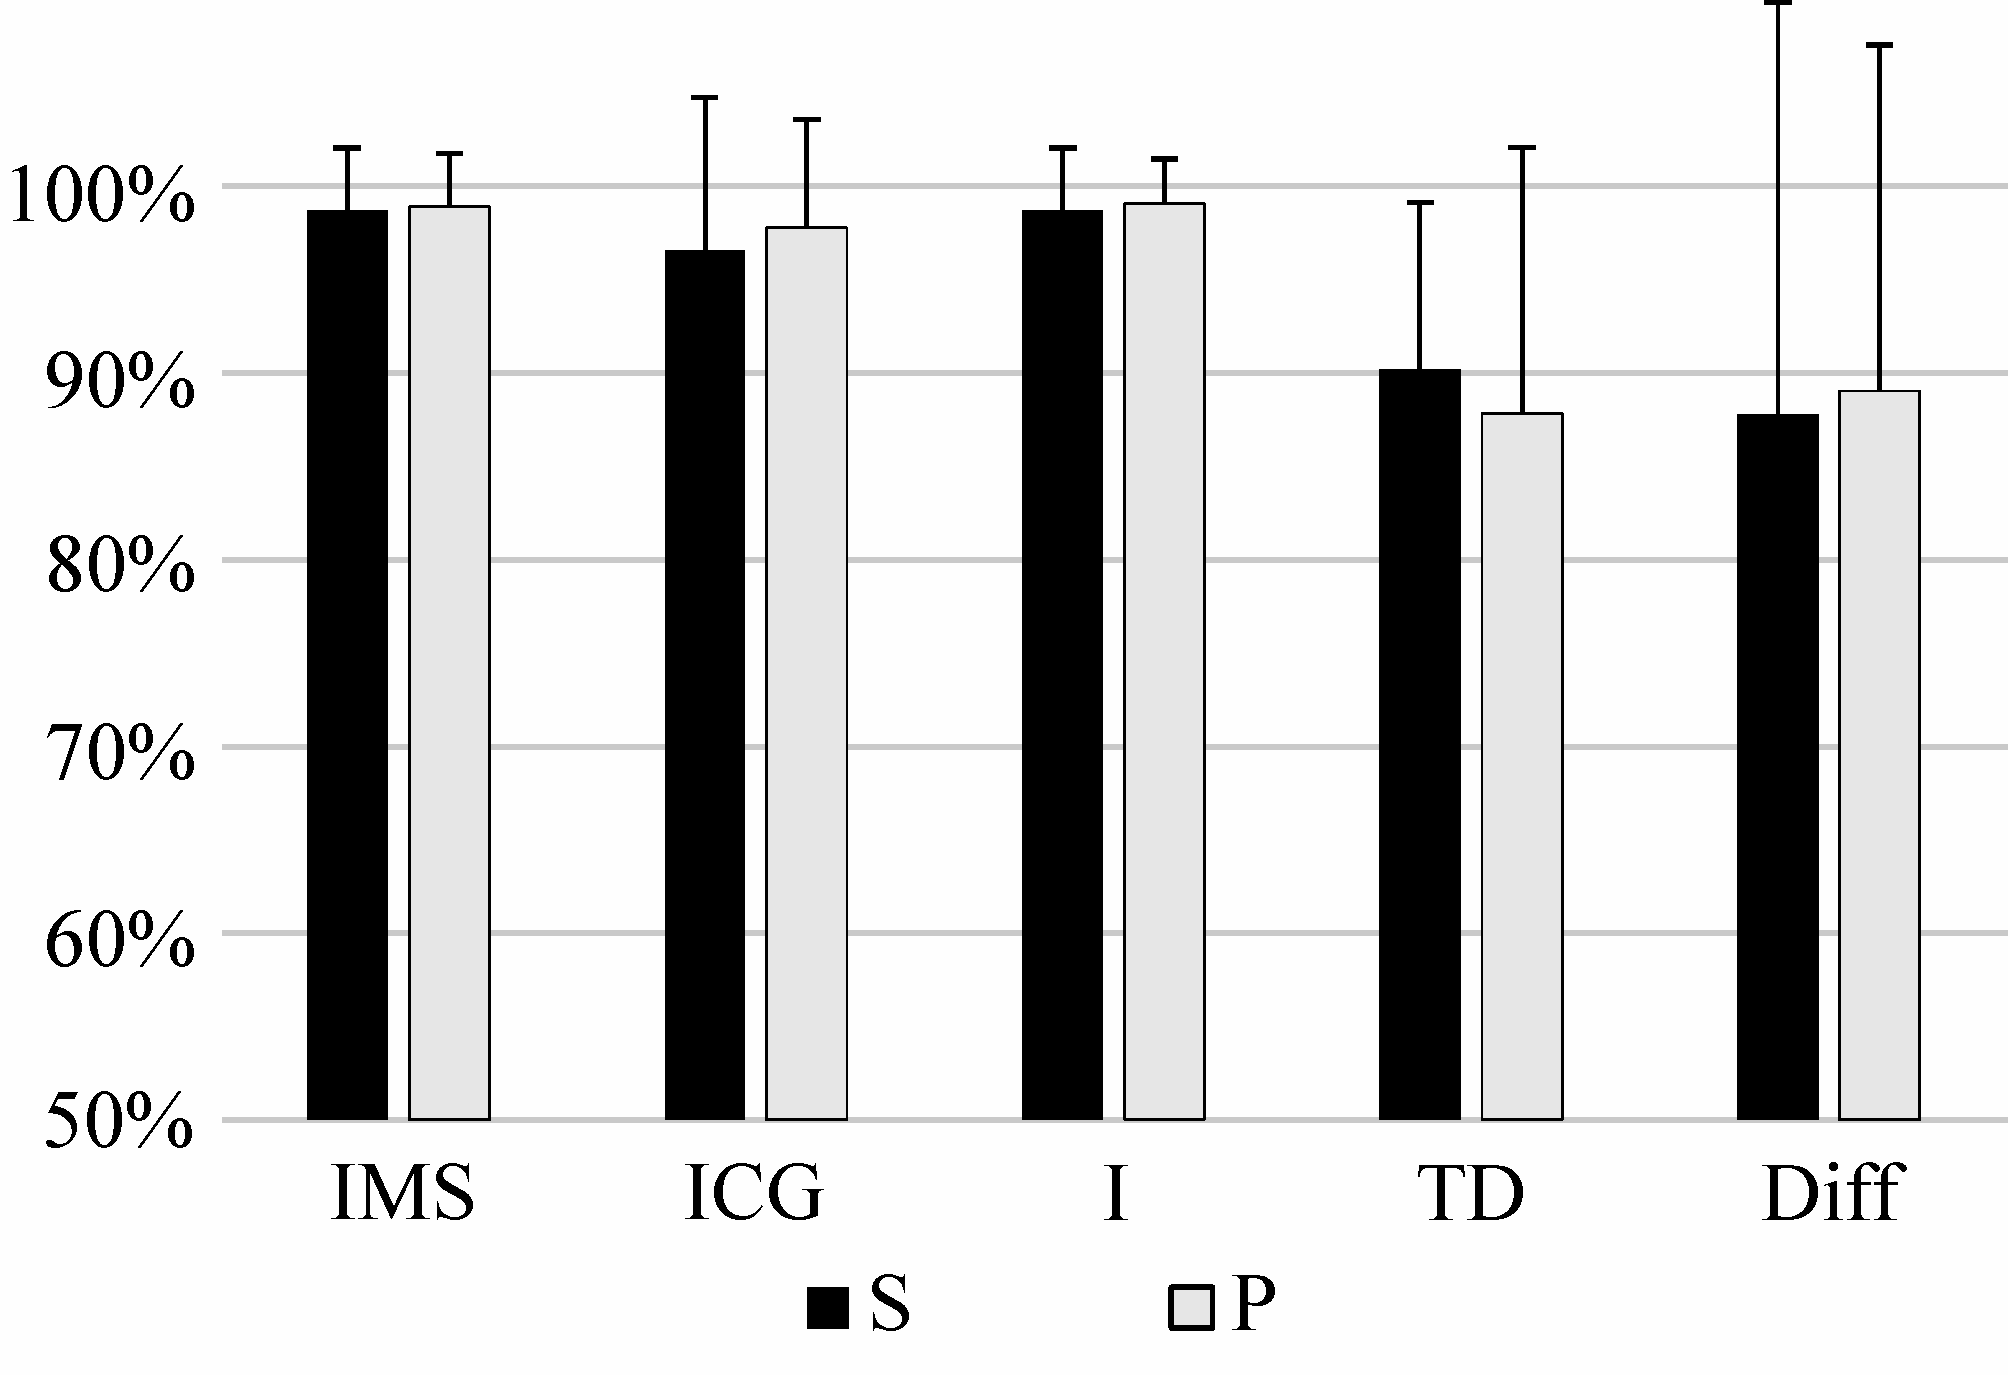
\includegraphics[width=0.45\textwidth]{Images/figure3_10.png}
\caption{Sensitivity (S) and precision (P) of long-term identification of task using IMS, ICG, I, TD, and Diff features.}
\label{fig:3-10}
\end{figure}   

\subsection{Identification during fatigue}
The influence of fatigue on EMG was evaluated using endurance recordings. Recordings were divided into five equal time epochs. The training set was obtained from the first epoch (0–20\% TDR), and the identification was performed on all five time epochs.
Changes of sensitivity and precision during the exercise can be seen in Figure \ref{fig:3-11}. It can be seen how all feature sets perform similarly at the beginning of the contraction, whereas identification indices decay towards the end as the fatigue accumulates. However at the final stages of fatigue (80\%–100\% TDR) IMS features significantly outperform other feature sets ($p < 0.05$). These results show the robustness of the IMS features to the fatigue.

\begin{figure}[ht]
\centering
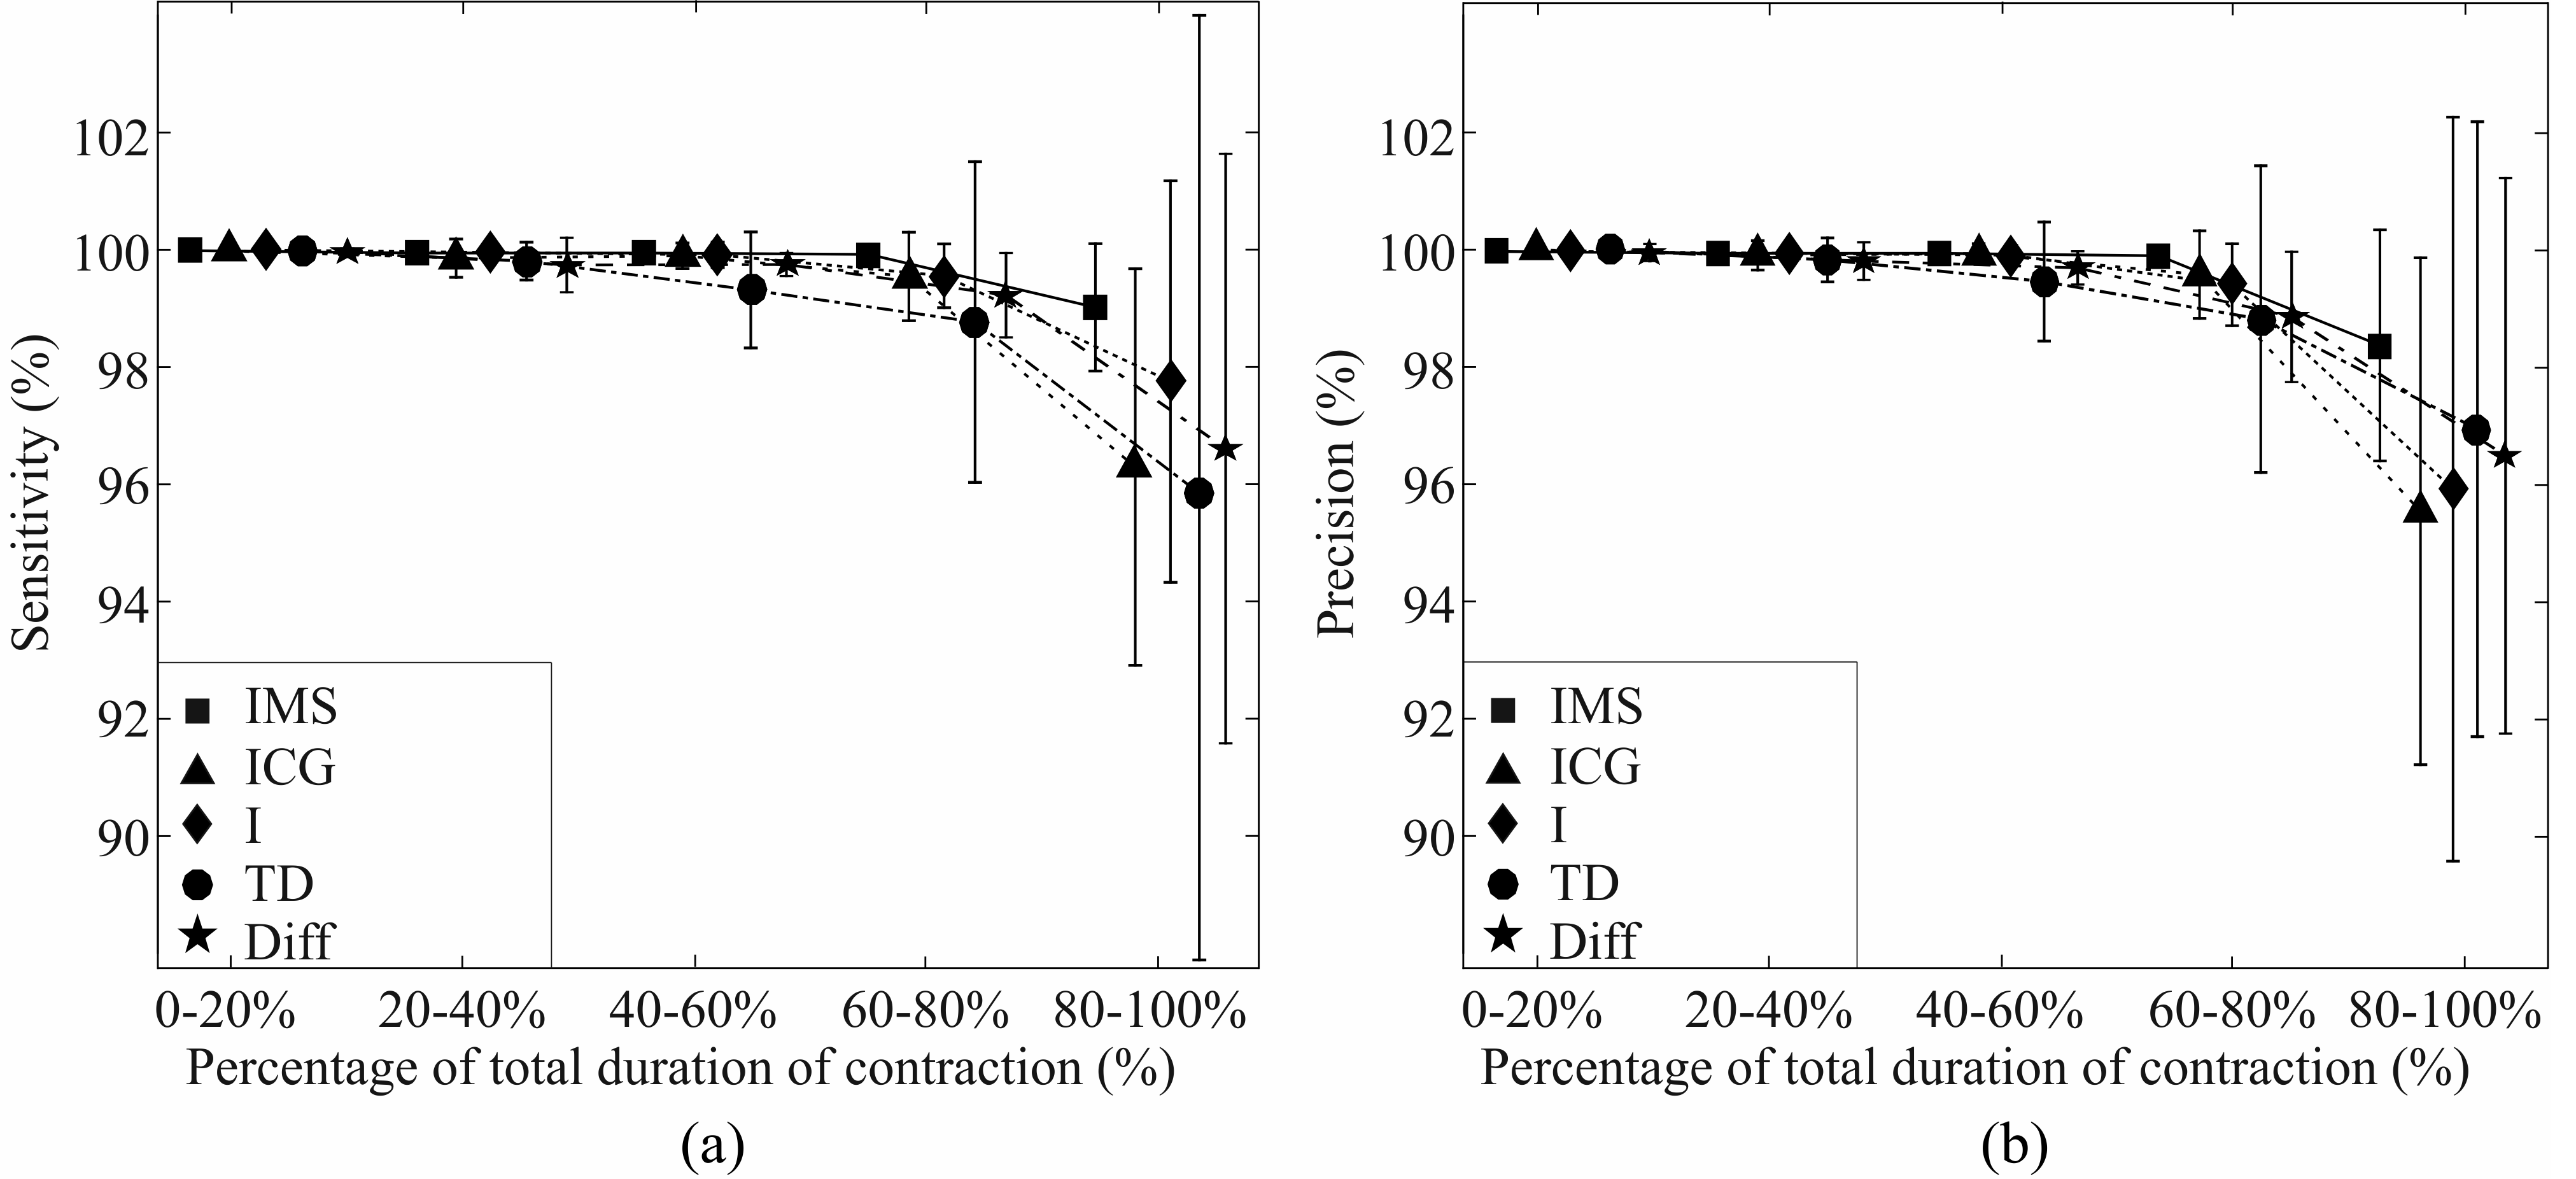
\includegraphics[width=0.9\textwidth]{Images/figure3_11.png}
\caption{Influence of fatigue on (a) sensitivity and (b) precision of the identification of task using IMS, ICG, I, TD, and Diff features.}
\label{fig:3-11}
\end{figure}   
\clearpage

\section{Discussion} \label{sc:3-4}
This study showed that the combination of intensity and spatial information is useful for the extraction of neuromuscular information. The spatial information was calculated from the RMS activation maps using the mean shift algorithm. Results were evaluated using the 70\% repeated holdout method and stratified sampling as to have sufficient number of samples of each class in the sets. To prevent the type III statistical error \citep{Mosteller1948, Mohebian2017}, a repeated hold-out was used. Sensitivity and precision, as appropriate unbiased measures in analyzing imbalanced multi-class problems \citep{Jordanic2016b, Rojas-Martinez2013}, were used to quantify the identification.

IMS features achieved very good results compared to other feature sets during task identification when the task was performed at very low effort level. Moreover, the Friedman test showed no significant differences in task identification using IMS when tasks were performed at 10\% MVC, 30\% MVC, or 50\% MVC. This can be a very important quality in everyday applications where subject could not need to contract muscles at moderate effort level to complete the task. It can be a step toward more natural control where even slight contractions can be successfully identified. In fact, only activations with low level of intensity are sometimes possible in patients with neuromuscular impairments.

A high identification rate is not the only factor important in the extraction of neural information from sEMG. The system should also be robust to slow time-dependent changes such as fatigue and electrode-skin contact impedance \citep{Farina2014}. Therefore, the robustness of the proposed features was tested with respect to time and fatigue. When evaluating the time effect, no significant differences in performance were found between IMS, ICG, and I feature sets and IMS significantly outperformed TD and Diff features. However, time effect was evaluated only when test set was composed of contractions recorded at 50\% MVC and, as shown in Figure \ref{fig:3-6}, all features perform similarly for the identification of that effort level. This phenomenon was already remarked and described in \citep{Jordanic2016a} where authors noted that adding spatial features to intensity features significantly improved the identification of tasks recorded at low effort levels, whereas improvement is not significant at moderate effort levels. On the other hand, the proposed features are particularly robust in task identification during fatiguing exercises and show significantly higher identification rate when compared to other features. Further improvements in reliability of the identification during the long-term contractions and fatiguing contractions can be achieved by using adaptive identification models that are being constantly updated during the usage, e.g., \citep{Vidovic2016, Hahne2015, Sensinger2009}.

In the current work, features were extracted from the RMS activation maps of the HD-EMG. Although these features proved to be very effective, by describing the EMG signal with its RMS value, i.e., the estimator of variance, the information is partially lost. Since the gradient of the probability density function of raw EMG is a useful feature in task identification, statistical measures (e.g., modes) of the raw HD-EMG, i.e., joint distribution of instantaneous EMG amplitude over the electrode array, could provide valuable information. Moreover, in literature, features were often calculated for each channel separately and selected using the simple sequential method prior to classification \citep{Hargrove2009, Li2017}. On the other hand, Geng et al. recently proposed a more advanced channel selection method based on common spatial patterns \citep{Geng2014}. Modes of the HD-EMG density function could be correlated with the channels with discriminative information and could be a useful tool in channel selection.

Finally, the mean shift algorithm can be used for clustering and, since it was shown that the algorithm is most effective in low-dimensional data, image segmentation is one of its most successful applications \citep{Comaniciu2002}. A mode of the density estimate, or in this case, a channel selected by the mean shift algorithm, can be considered as a cluster representative \citep{Hennig2015}, related to the possible image segments, where spatial (pixel locations) and range features (the intensity of the grayscale value) are considered. The advantage of the mean shift is that it can be used for clustering non-convex shapes, albeit, it could segment complex non-convex regions in the activation maps. Since segmentation of the muscle activation map can improve the neuromuscular activity estimation \citep{Vieira2010}, this could be a reason why mean shift features improved the performance of the movement detection system compared with previously published attributes. In addition, the algorithm only requires setting one parameter, bandwidth ($h$) and, unlike in the similar methods, it is not necessary to define the number of expected clusters. This is a big advantage because it does not require a priori knowledge on the number of clusters.

As a limitation of the study, it should be noted that the proposed features were tested only in highly controlled conditions of isometric contractions. The experiments during non-isometric contractions should be performed in order to validate the quality of the features in dynamic and more natural movements. Also, the experiment included only four tasks related to the elbow joint. Further analysis should include higher number of more complex tasks related to hand and shoulder. Moreover, all results were obtained during offline analysis. To evaluate practical aspects of the features, the experiment should be repeated using online identification and considering multiple transitions between tasks.


\section{Conclusions} \label{sc:3-5}
In conclusion, a new set of features for the identification of isometric motor tasks of upper limb was proposed. It was based on the combination of intensity and the spatial distribution of intensity of HD-EMG. These new features were evaluated using the LDA classifier and the results showed they improve the identification of tasks. Moreover, robustness of the features was tested under the influence of slow time-dependent changes of the EMG. They proved to be particularly useful for task identification when muscles were fatigued. The proposed methods could be used for the design and monitoring of rehabilitation therapies intended for patients with neuromuscular impairment, as well as for the control of external devices like exoskeletons, and prostheses.


\section{Acknowledgments}
Special acknowledgement to Laboratory of Engineering of Neuromuscular System and Motor Rehabilitation at the Politecnico di Torino for the help and collaboration during the experiments. This work has been partially supported by the Spanish Ministry of Economy and Competitiveness (Project DPI2014-59049-R), People Programme (Marie Curie Actions) of the Seventh Framework Programme of the European Union (FP7/2007-2013) under REA grant agreement no. 600388 (TECNIO spring programme), and by the grant for the recruitment of early-stage research staff (FI 2014) from the AGAUR, Generalitat de Catalunya, Spain.


\section{Author contributions}
M.R.-M. and M.A.M. conceived and designed the experimental protocol and conducted the experiments. M.J., M.R.M. and M.A.M. designed the study and interpreted the results. M.J. was in charge of the implementation of signal processing and machine learning methods and the analysis of the data. J.F.A. and H.R.M. aided in the analysis of the data and in the interpretation of results. M.J. wrote the manuscript and all authors contributed to the revising it.

\section{Conflicts of interest}
The authors declare no conflict of interest.
\clearpage

\section{Appendix A}
The mean shift algorithm is a non-parametric approach to estimate the gradient of a density function. It was first proposed by \citet{Fukunaga1975}, but did not get a lot of attention of the academic community initially. Although their work was cited more than 1500 times in literature, most of the cites occurred after the famous publication of Comaniciu and Meer in 2002 (counting almost 6000 citations) that revised the method and drew attention of the scientific community to it \citep{Comaniciu2002}.

The algorithm is the enhanced version of the Parzen window technique for the estimation of density using a kernel \citep{Parzen1962} and its extension to multivariate distributions \citep{Cacoullos1966}, given that density for the point $\textbf{x}$ can be estimated based on the observed samples $\textbf{x}_i$ $(i = 1,2,…,n)$ using the kernel function $K$ as:
\begin{equation} \label{eq:3-A1}
\hat{f}(\mathbf{x}) = \frac{1}{n} \sum_{i=1}^{n} K_{H} (\mathbf{x}-\mathbf{x}_i)
\end{equation}
\begin{equation} \label{eq:3-A2}
K_H =  \vert \mathbf{H} \vert ^{-\frac{1}{2}} K (\mathbf{H}^{-\frac{1}{2}} \mathbf{x})
\end{equation}
, where $\hat{f}(\mathbf{x})$ is the estimated density, $K_H$ is the normalized kernel function, and $H$ is $d x d$ bandwidth matrix. The bandwidth matrix $H$ can be fully parameterized, diagonal, or, as in this paper, proportional to identity matrix $(\mathbf{H} = h\mathbf{I})$, which simplifies the expression for the density estimation to:
\begin{equation} \label{eq:3-A3}
\hat{f}(\mathbf{x}) = \frac{1}{nh^d} \sum_{i=1}^{n} K (\frac{\mathbf{x}-\mathbf{x}_i}{h})\
\end{equation}
, where $\hat{f}(\mathbf{x})$ is the estimated density, $h$ is a single bandwidth parameter, $d$ is the number of dimensions, and $K$ is the kernel function. Two commonly used univariate kernel profiles are Epanechnikov $(k_E)$ and Gaussian $(k_N)$:
\begin{equation} \label{eq:3-A4}
k_N (x) = e^{- \frac{1}{2} x},\,\, x \geq 0
\end{equation}
\begin{equation} \label{eq:3-A5}
k_E (x) = \left\{\begin{array}{lr} 1-x & \,\,0 \leq x \leq 1\\ 0  & \,\,x > 1 \ \end{array}\right.
\end{equation}
, which yield multivariate radially symmetric kernel $(K_E)$ and normal kernel $(K_N)$ respectively:
\begin{equation} \label{eq:3-A6}
K_N ( \mathbf{x}) = \frac{1}{2 \pi^{d/2}} e^{- \frac{1}{2} \parallel \mathbf{x} \parallel^2}
\end{equation}
\begin{equation} \label{eq:3-A7}
K_E ( \mathbf{x}) = \left\{\begin{array}{lr} \frac{1}{2} \frac{d+2}{c_d} \left(1 - \parallel \mathbf{x}\parallel^2\right) & \,\, \parallel \mathbf{x}\parallel \leq 1    \\
 0  & \,\,\parallel \mathbf{x}\parallel > 1 \end{array}\right.
\end{equation}
, where $d$ is the number of dimension and $c_d$ is the constant that ensures the kernel integrates to one.

Mean shift vector is defined as \citep{Comaniciu2002}:
\begin{equation} \label{eq:3-A8}
\mathbf{ms} (\mathbf{x}) = 
\frac{\sum_{i=1}^n \, \mathbf{x}_i \, g (\parallel  \frac{\mathbf{x}-\mathbf{x_i}}{h} \parallel^2) }{\sum_{i=1}^n \, g (\parallel  \frac{\mathbf{x}-\mathbf{x}_i}{h} \parallel^2)} - \mathbf{x}
\end{equation}
,where $g(x)$ is the negative derivative of the original univariate kernel profile $k(x)$:
\begin{equation} \label{eq:3-A9}
g(x) = - \frac{dk(x)}{dx}
\end{equation}

Mean shift is a function defined for every point in space. It is a vector of difference between the current position and the weighted mean of all points within its bandwidth $h$, whose weights are defined by the kernel profile $g(x)$. Therefore, the mean shift vector always points to the direction of maximum increase of the density and can be considered as a function proportional to the gradient of the density function:
\begin{equation} \label{eq:3-A10}
\mathbf{ms}_g (\mathbf{x}) \, \propto \, \nabla \hat{f}_k (\mathbf{x})
\end{equation}

In addition, mean shift can be effectively used to find modes (local maxima) of the underlying density function by an iterative procedure. Kernel is usually centered at a random point in space and the mean shift vector is calculated. In the next iteration, the kernel is centered at the location pointed by the mean shift vector. The procedure is mathematically defined as:
\begin{equation} \label{eq:3-A11}
\mathbf{y}_{i+1} \coloneqq 
\frac{\sum_{j=1}^n \, \mathbf{x}_j \, g (\parallel \frac{\mathbf{y}_i-\mathbf{x}_j}{h} \parallel^2) }
{\sum_{j=1}^n \, g (\parallel  \frac{\mathbf{y}_i-\mathbf{x}_j}{h} \parallel^2)}
\end{equation}

By repeating this procedure, at every step, the center of the kernel is shifted to the direction of maximum increase of the density function until the local maximum is reached. At this location, the difference between two consecutive points is zero (up to a tolerance). These final stationary points are considered to be modes of the probability density function:
\begin{equation} \label{eq:3-A12}
\mathbf{y}_{i+1} - \mathbf{y}_i = 0
\end{equation}
\begin{equation} \label{eq:3-A12}
\mathbf{y}_{i+1} - \mathbf{y}_i = 0
\end{equation}
\begin{equation} \label{eq:3-A13}
\mathbf{ms}_g (\mathbf{y}_{i}) = \nabla \hat{f}_k \, (\mathbf{y}_i) = 0
\end{equation}

This algorithm is very useful in image processing and feature space analysis with many applications, of which clustering is the most popular. It only requires setting one parameter, bandwidth $(h)$. On the other hand, unlike the similar methods, e.g., $k-$ means clustering, it is not necessary to define the number of expected clusters. This is a big advantage because it does not require \textit{a priori} knowledge on the number of clusters. Detailed explanation of the mean shift algorithm can be found in the literature \citep{Comaniciu2002, Fukunaga1975}.

In this study, modes of the density function of root-mean-square (RMS) activation maps were found using the mean shift algorithm implemented in Python \citep{scikit-learn} and were used as features in the identification. The Epanechnikov kernel profile was employed to describe the density function, which yielded flat kernel profile $g(x)$ in the calculation of the mean shift vector:
\begin{equation} \label{eq:3-A14}
g (x) = \left\{\begin{array}{lr} 1, & \,\, \parallel x \parallel \leq h \\
0,  & \,\,\parallel x \parallel > h \end{array}\right.
\end{equation}

This choice of the kernel profile simplified the update of the mean shift centroid to:
\begin{equation} \label{eq:3-A15}
\left. \mathbf{y}_{i+1} \coloneqq \frac{\sum_{j=1}^{N} \mathbf{x}_j}{N} \right\vert_{\forall \mathbf{x} \,s.t. \,\parallel \mathbf{x}-\mathbf{y}_i \parallel \leq h}
\end{equation}
In the other words, the new centroid was calculated as the mean value of $N$ points located within the Euclidean distance $h$ from the current centroid.
\clearpage


\section{Appendix B}\label{Apx B}
Example of the torque signals during supination and pronation can be seen in the Figure \ref{fig:3-B1}, along with the EMG signal recorded on pronator teres. It is possible to observe that the polarity of the torque signals change depending on the direction of the movement. The mechanical brace is fixed at the wrist so that the exerted force during supination and pronation is monitored by left and right torque meters, respectively. In addition, as expected, the amplitude of the sEMG signal in the Pronator Teres is higher during pronation.

\begin{figure}[ht]
\centering
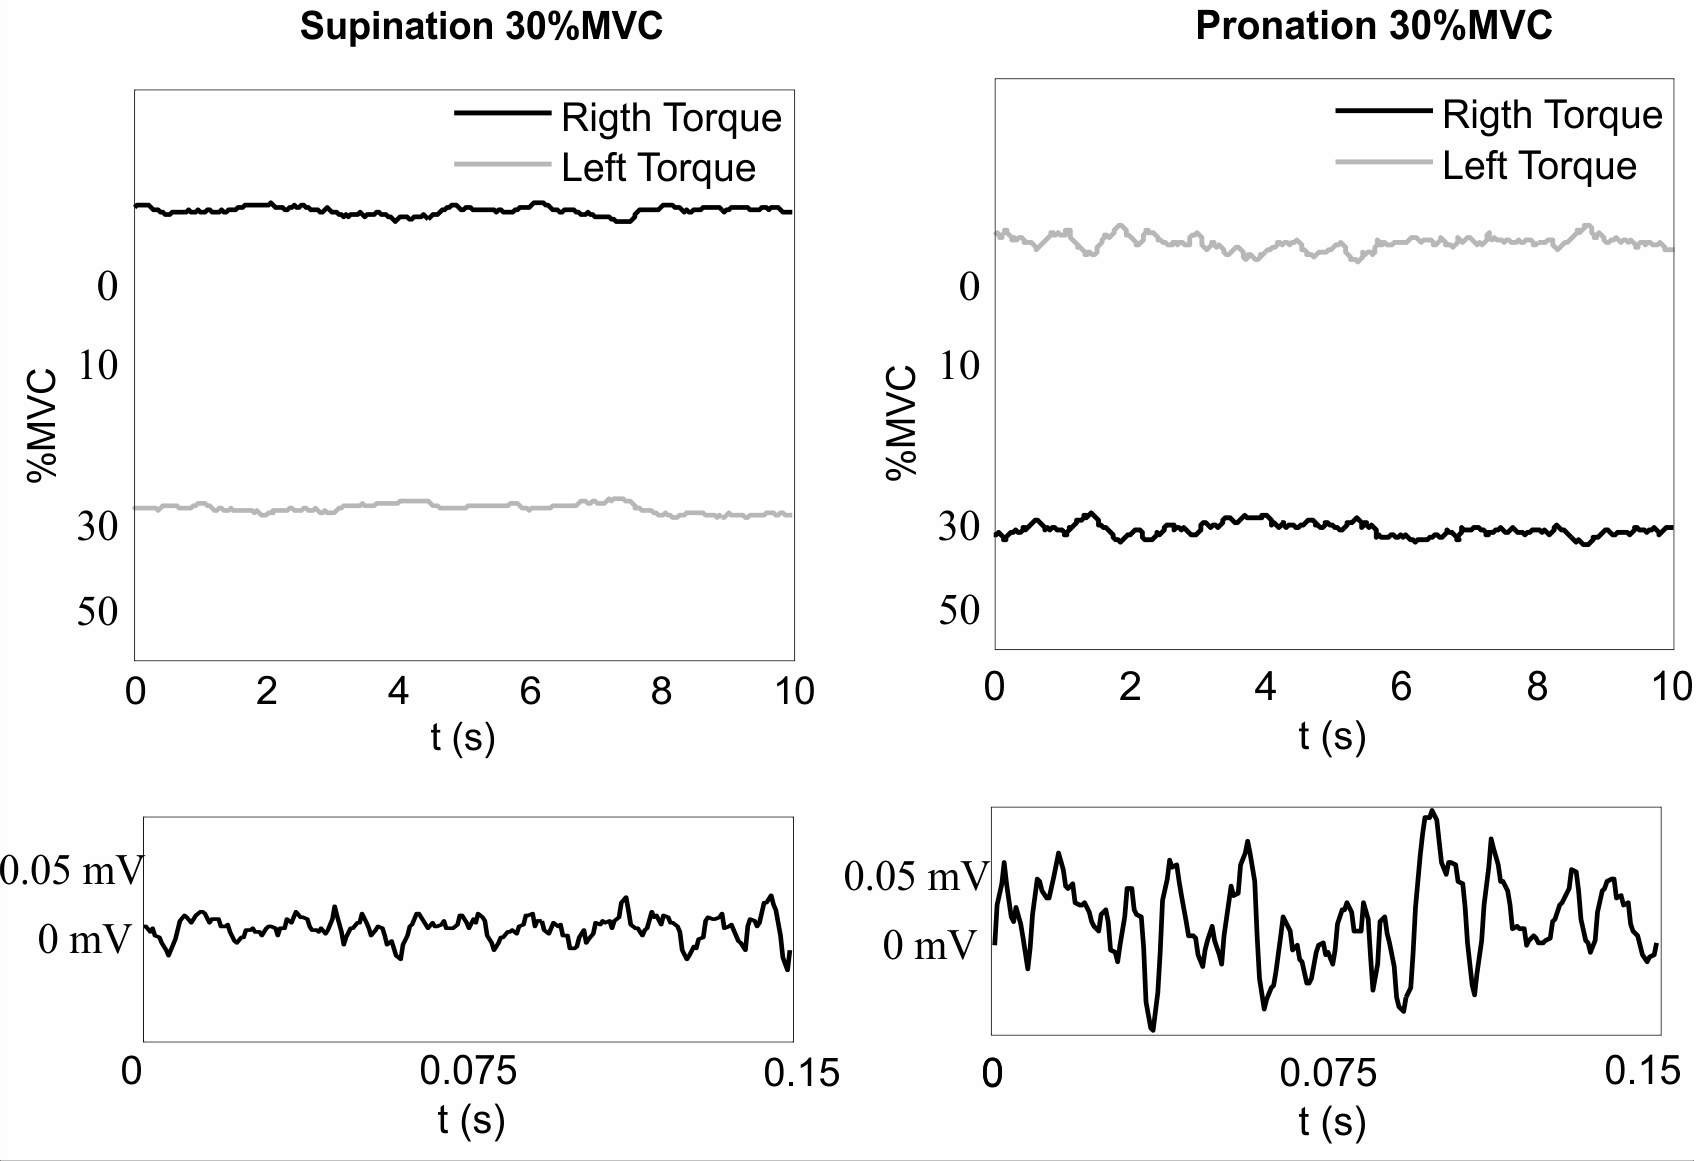
\includegraphics[width=0.9\textwidth]{Images/figure3_B1.png}
\caption{Example of torque and EMG signals in supination and pronation in one subject. Left. Supination at 30\% MVC. The exerted torque on right (black) and left (gray) sides of the mechanical brace are shown at the top of the figure. The sEMG signal recorded on one of the channels of the Pronator Teres muscle is shown at the bottom. Rigth. Torque signals for Pronation at 30\% MVC are shown on the top of the figure. The sEMG signal recorded on the same channel as in the previous case is shown at the bottom.}
\label{fig:3-B1}
\end{figure}   


On the other hand, examples of EMG signals recorded on five muscles during 30\% MVC flexion, extension, supination, and pronation can be seen in Figure \ref{fig:3-B2}, Figure \ref{fig:3-B3}, Figure \ref{fig:3-B4} and Figure \ref{fig:3-B5}, respectively. Figures show raw EMG signals and signals filtered using 4\textsuperscript{th} order Butterworth filter with cut-off frequencies of of 15 Hz and 350 Hz. Scale for each muscle is the same across different tasks to show difference in EMG amplitudes in dependence of task.

\begin{figure}[ht]
\centering
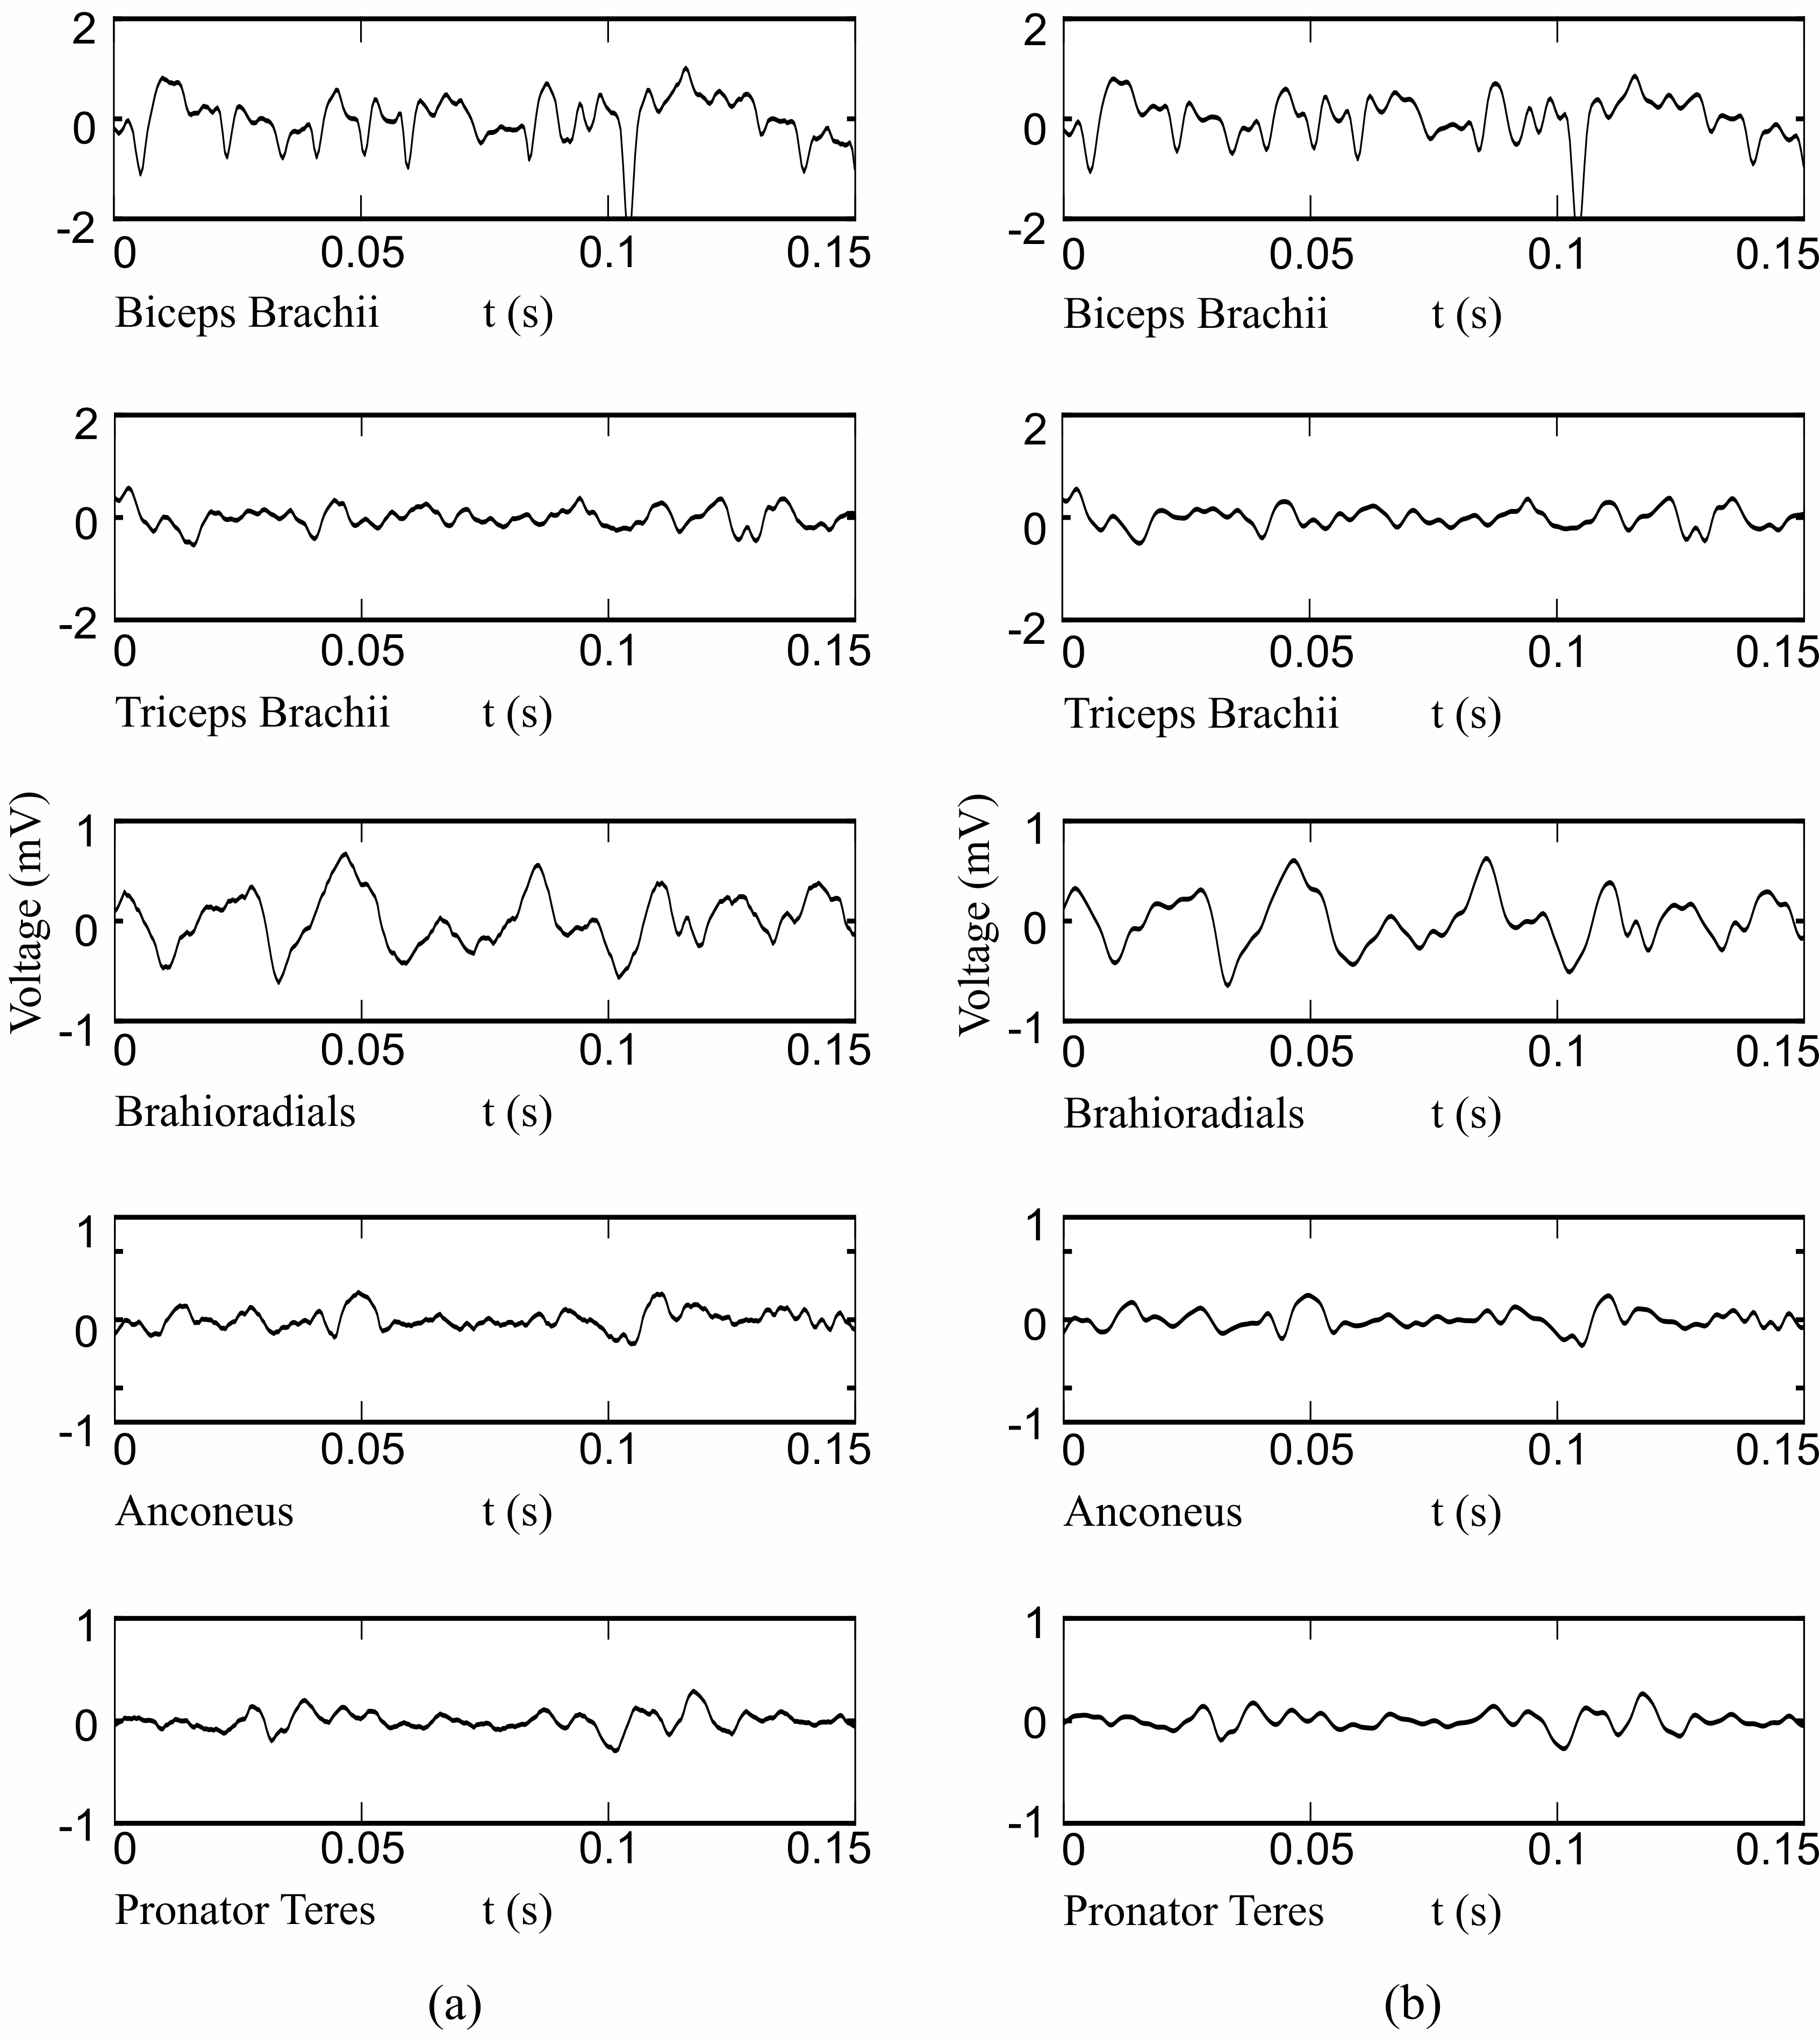
\includegraphics[width=0.99\textwidth]{Images/figure3_B2.png}
\caption{Examples of recorded EMG signals from five muscles (biceps brachii, triceps brachi, brachioradialis, anconeus, bracioradialis, and pronator teres) during flexion. Figure shows (a) raw signals and (b) signals filtered using 4\textsuperscript{th} order Butterworth filter with the cut-off frequencies of 15 Hz and 350 Hz.}
\label{fig:3-B2}
\end{figure}   

\begin{figure}[ht]
\centering
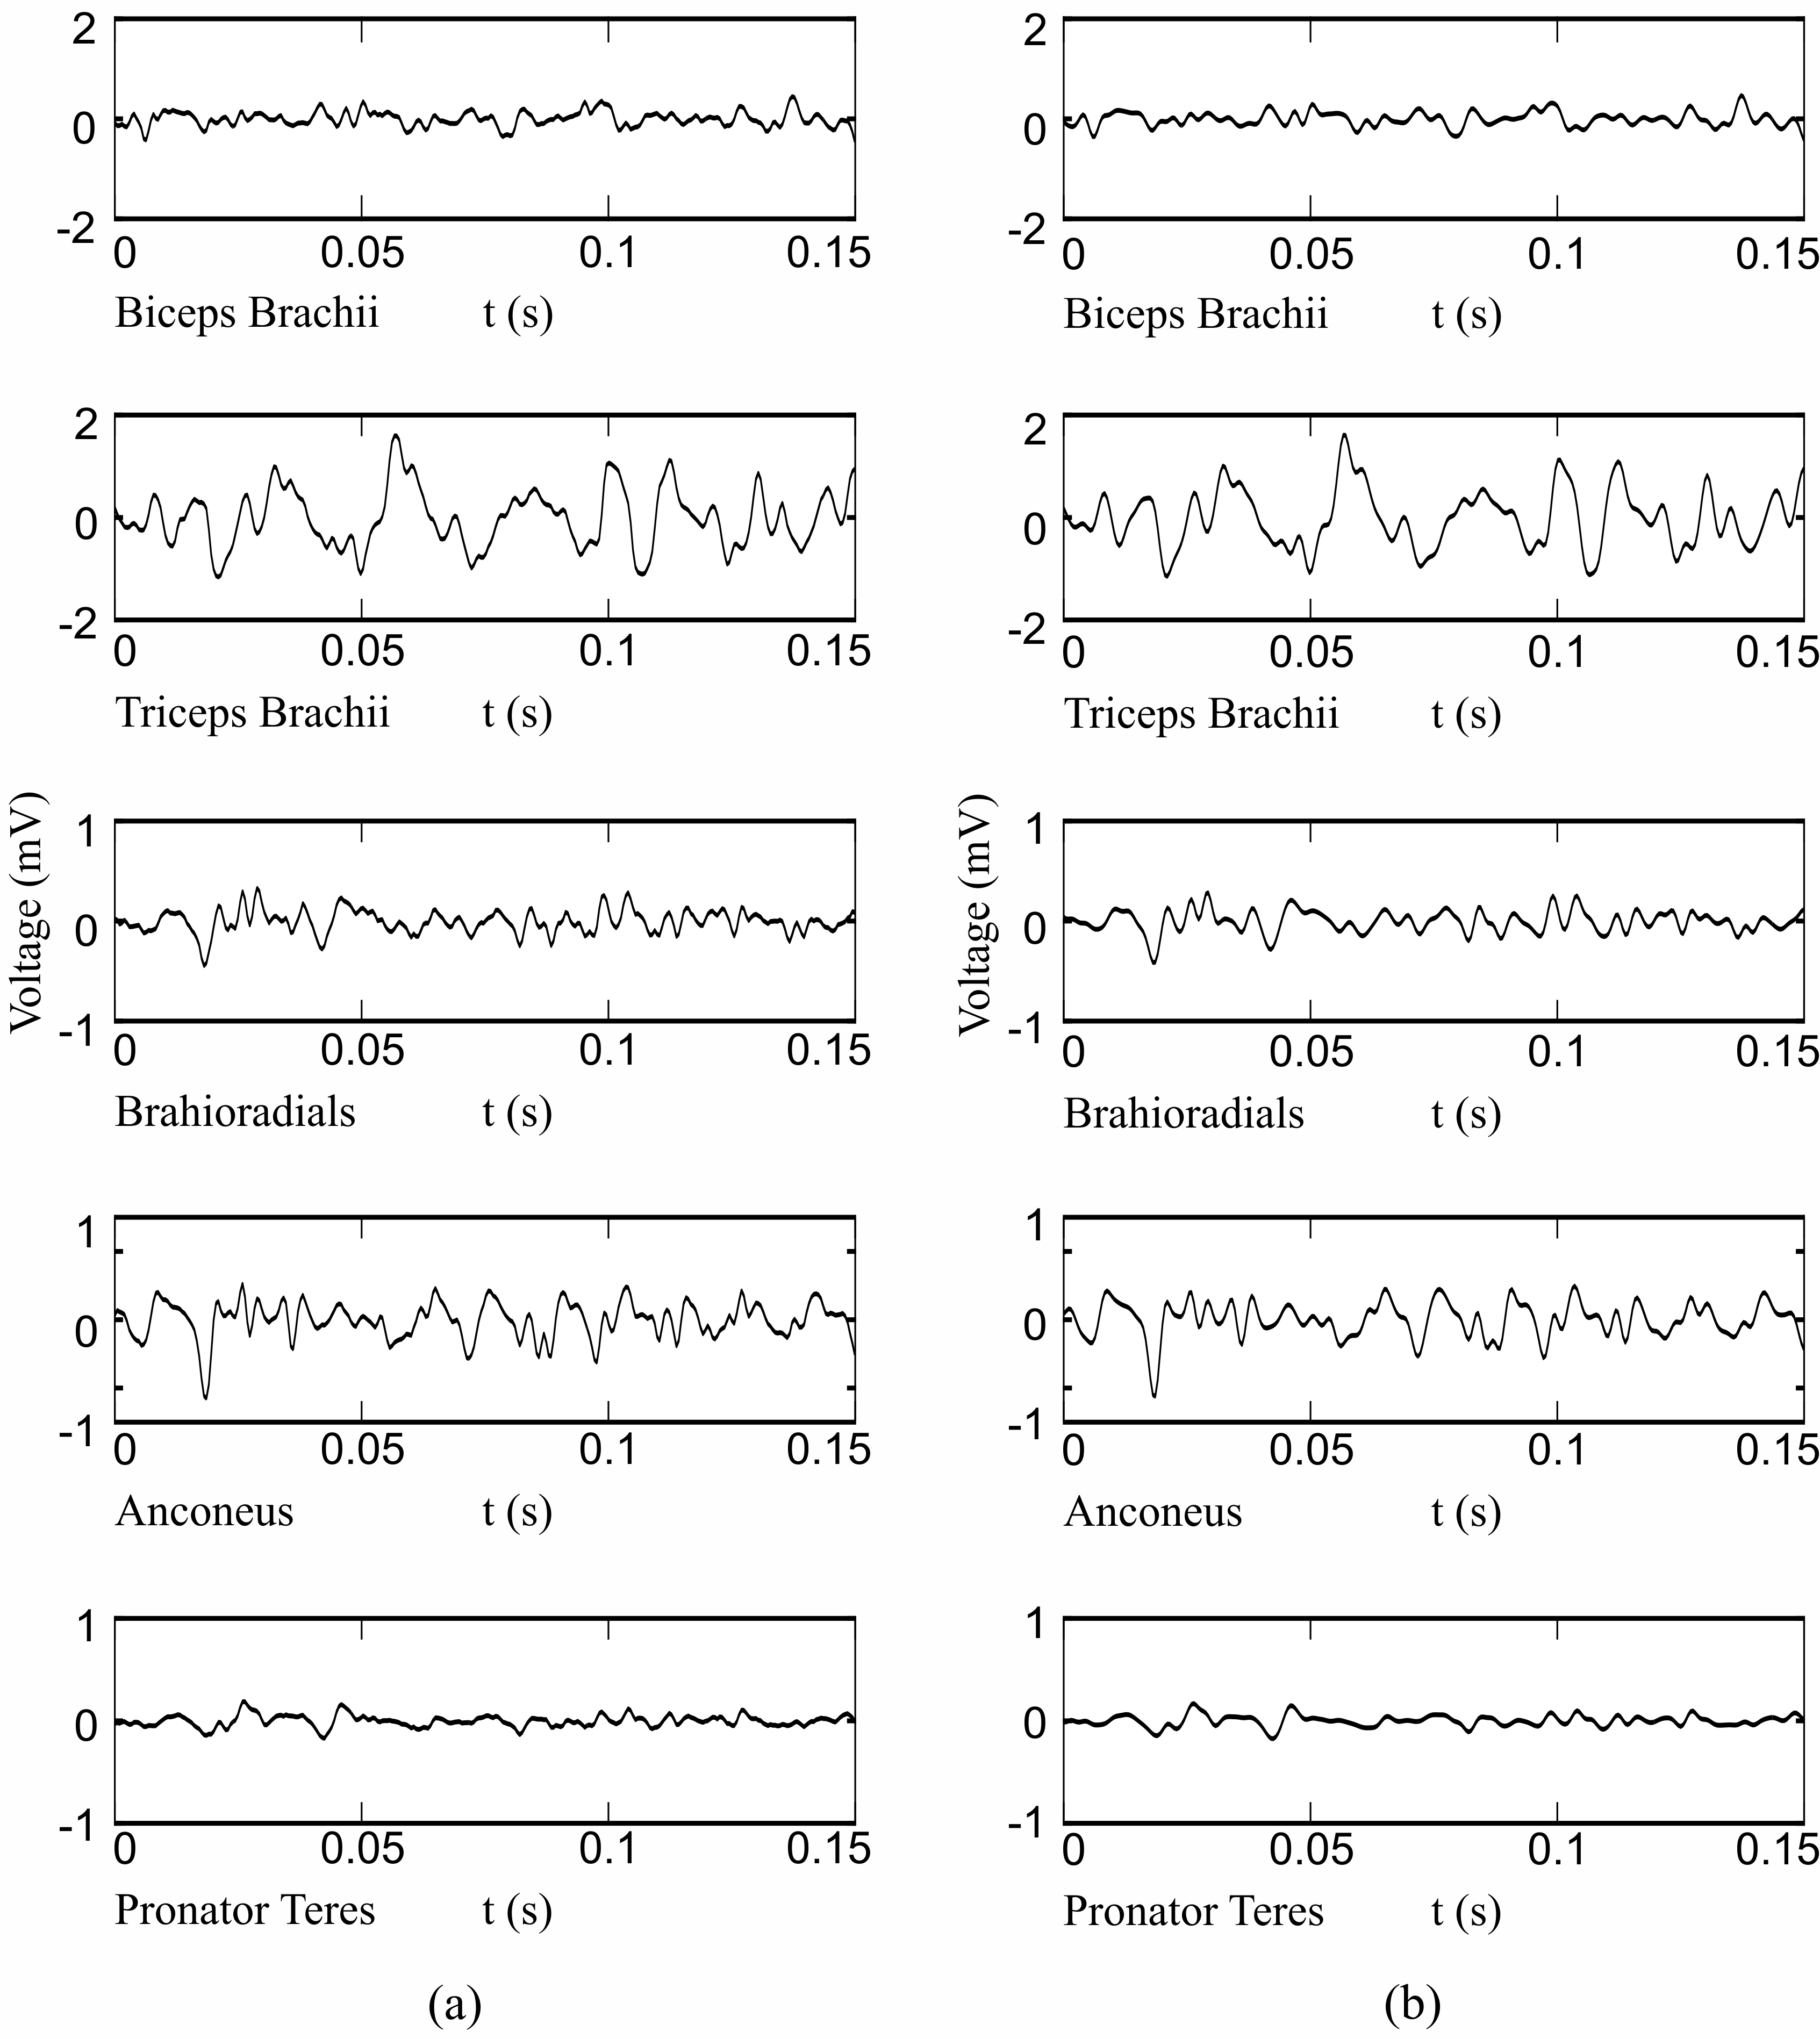
\includegraphics[width=0.99\textwidth]{Images/figure3_B3.png}
\caption{Example of recorded EMG signals from five muscles (biceps brachii, triceps brachi, brachioradialis, anconeus, bracioradialis, and pronator teres) during extension. Figure shows (a) raw signals and (b) signals filtered using 4\textsuperscript{th} order Butterworth filter with the cut-off frequencies of 15 Hz and 350 Hz.}
\label{fig:3-B3}
\end{figure}   

\begin{figure}[ht]
\centering
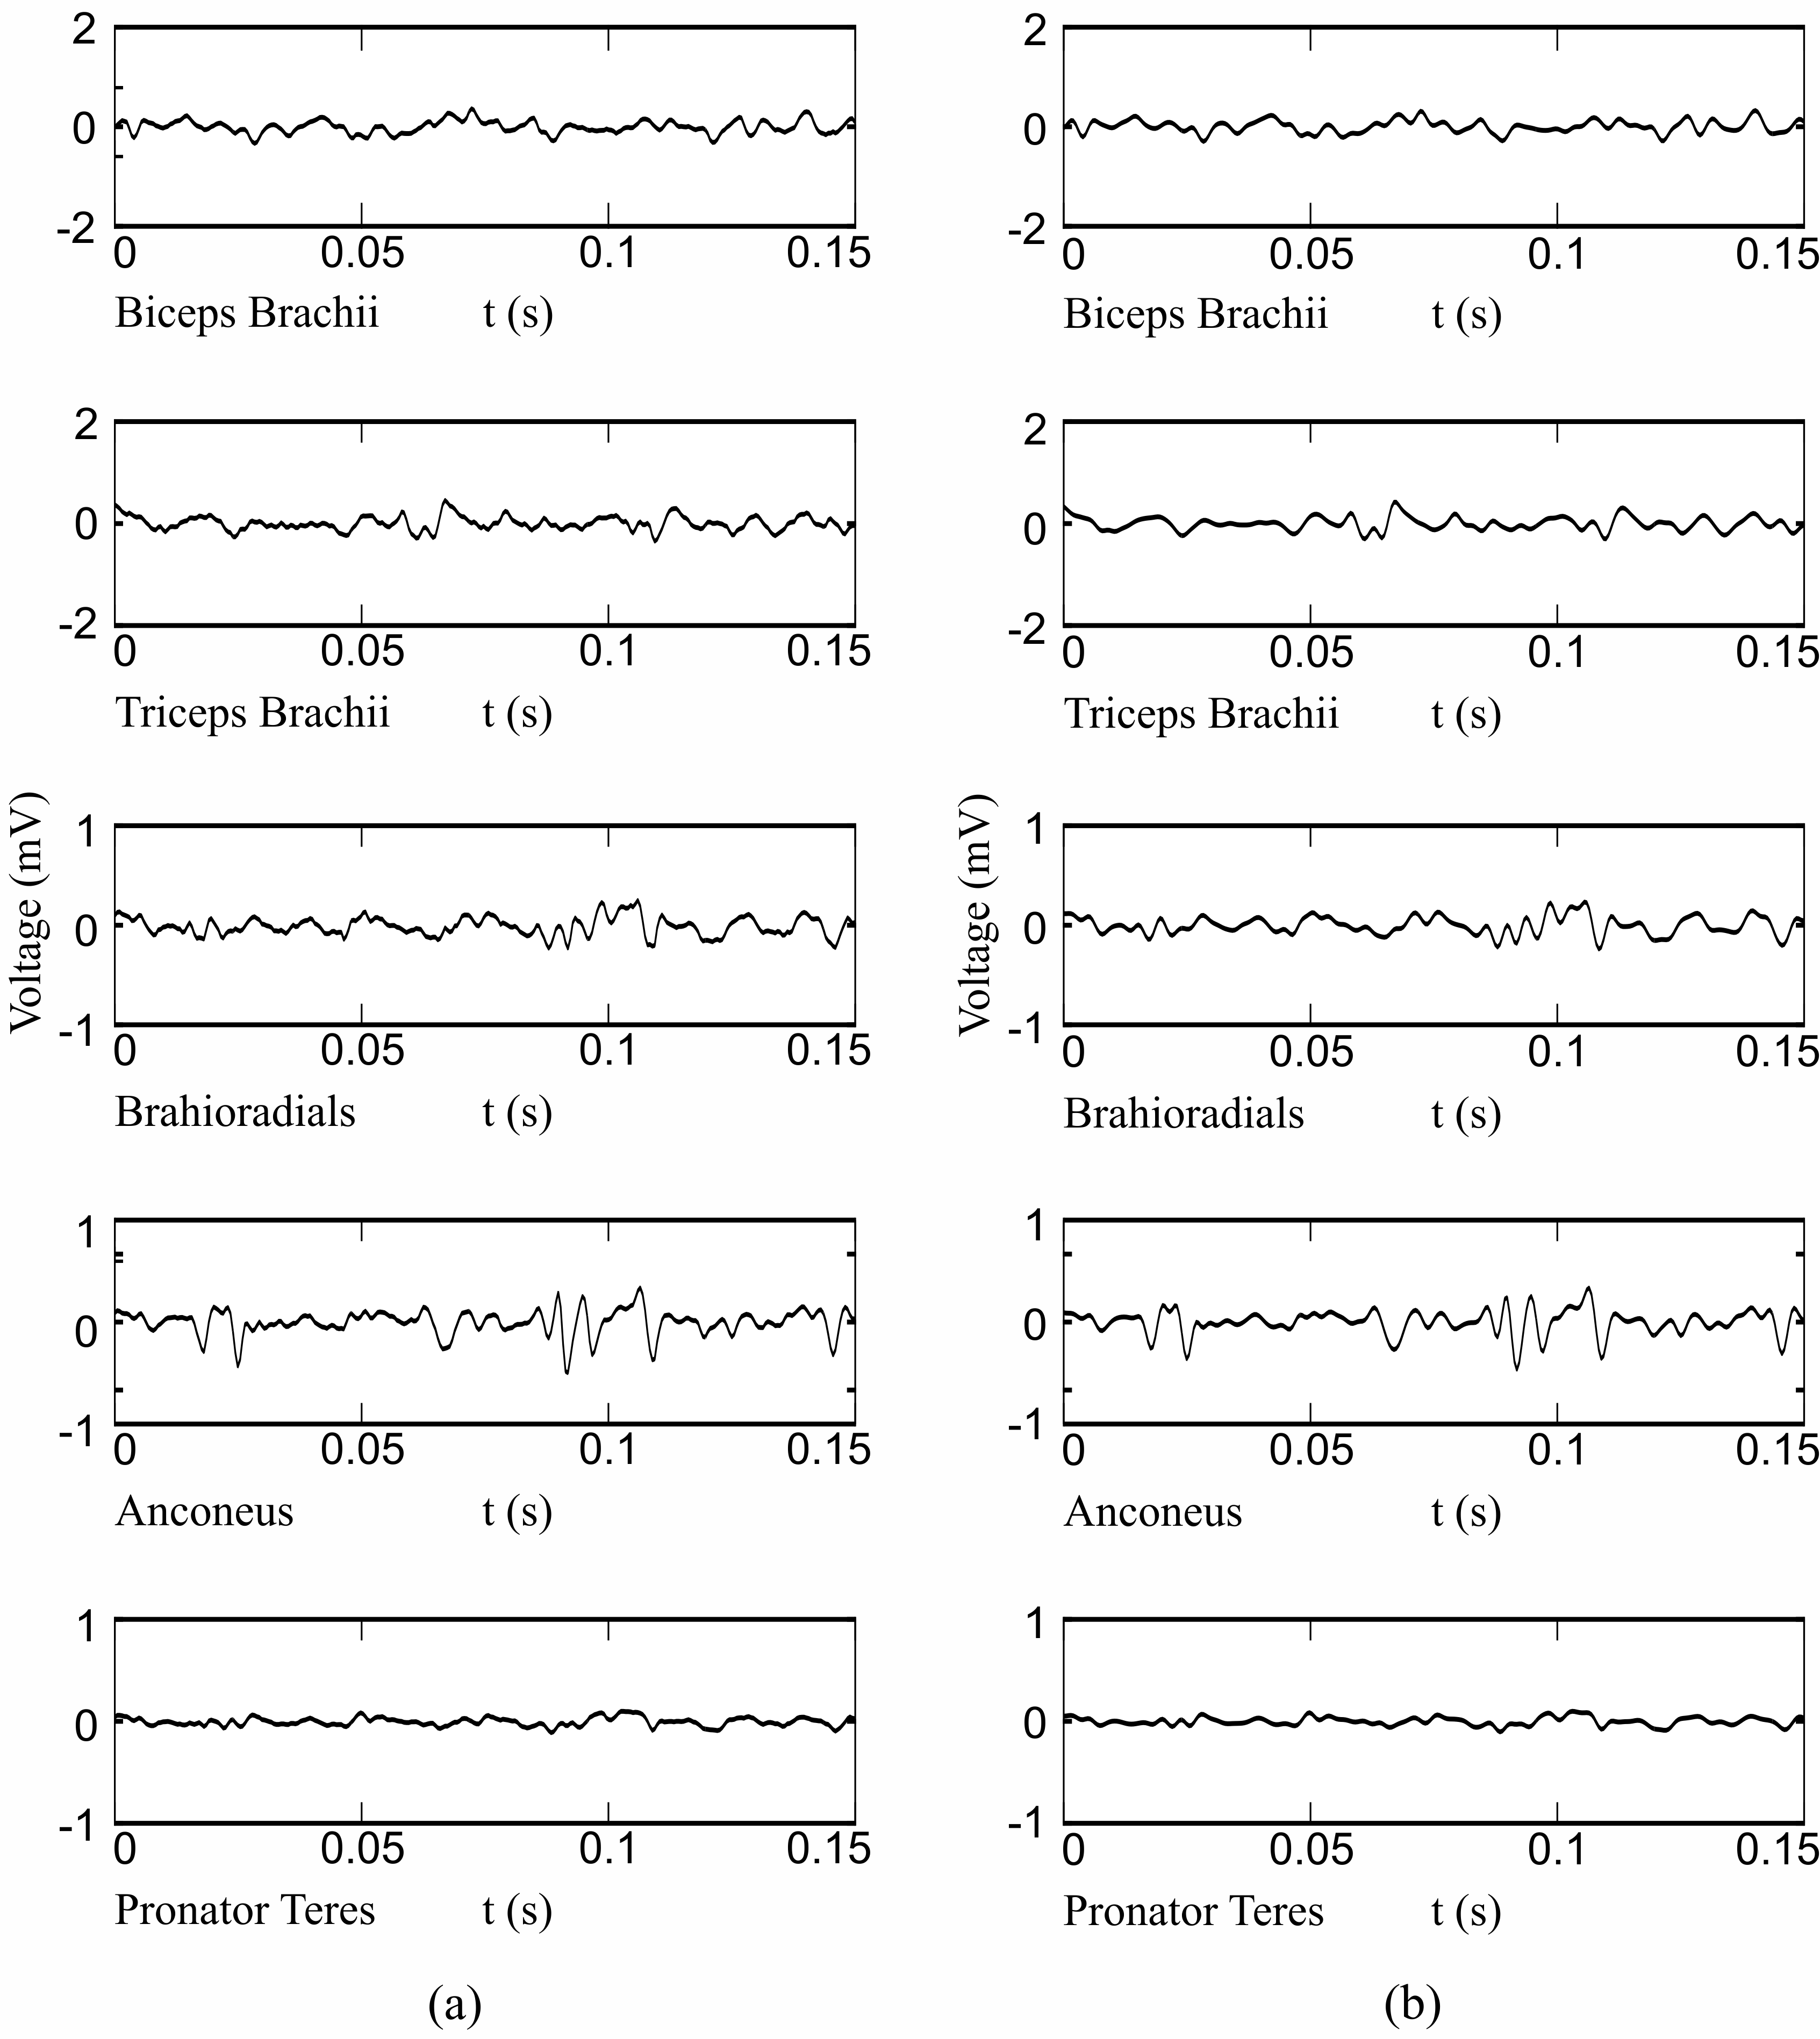
\includegraphics[width=0.99\textwidth]{Images/figure3_B4.png}
\caption{Example of recorded EMG signals from five muscles (biceps brachii, triceps brachi, brachioradialis, anconeus, bracioradialis, and pronator teres) during supination. Figure shows (a) raw signals and (b) signals filtered using 4\textsuperscript{th} order Butterworth filter with the cut-off frequencies of 15 Hz and 350 Hz.}
\label{fig:3-B4}
\end{figure}   

\begin{figure}[ht]
\centering
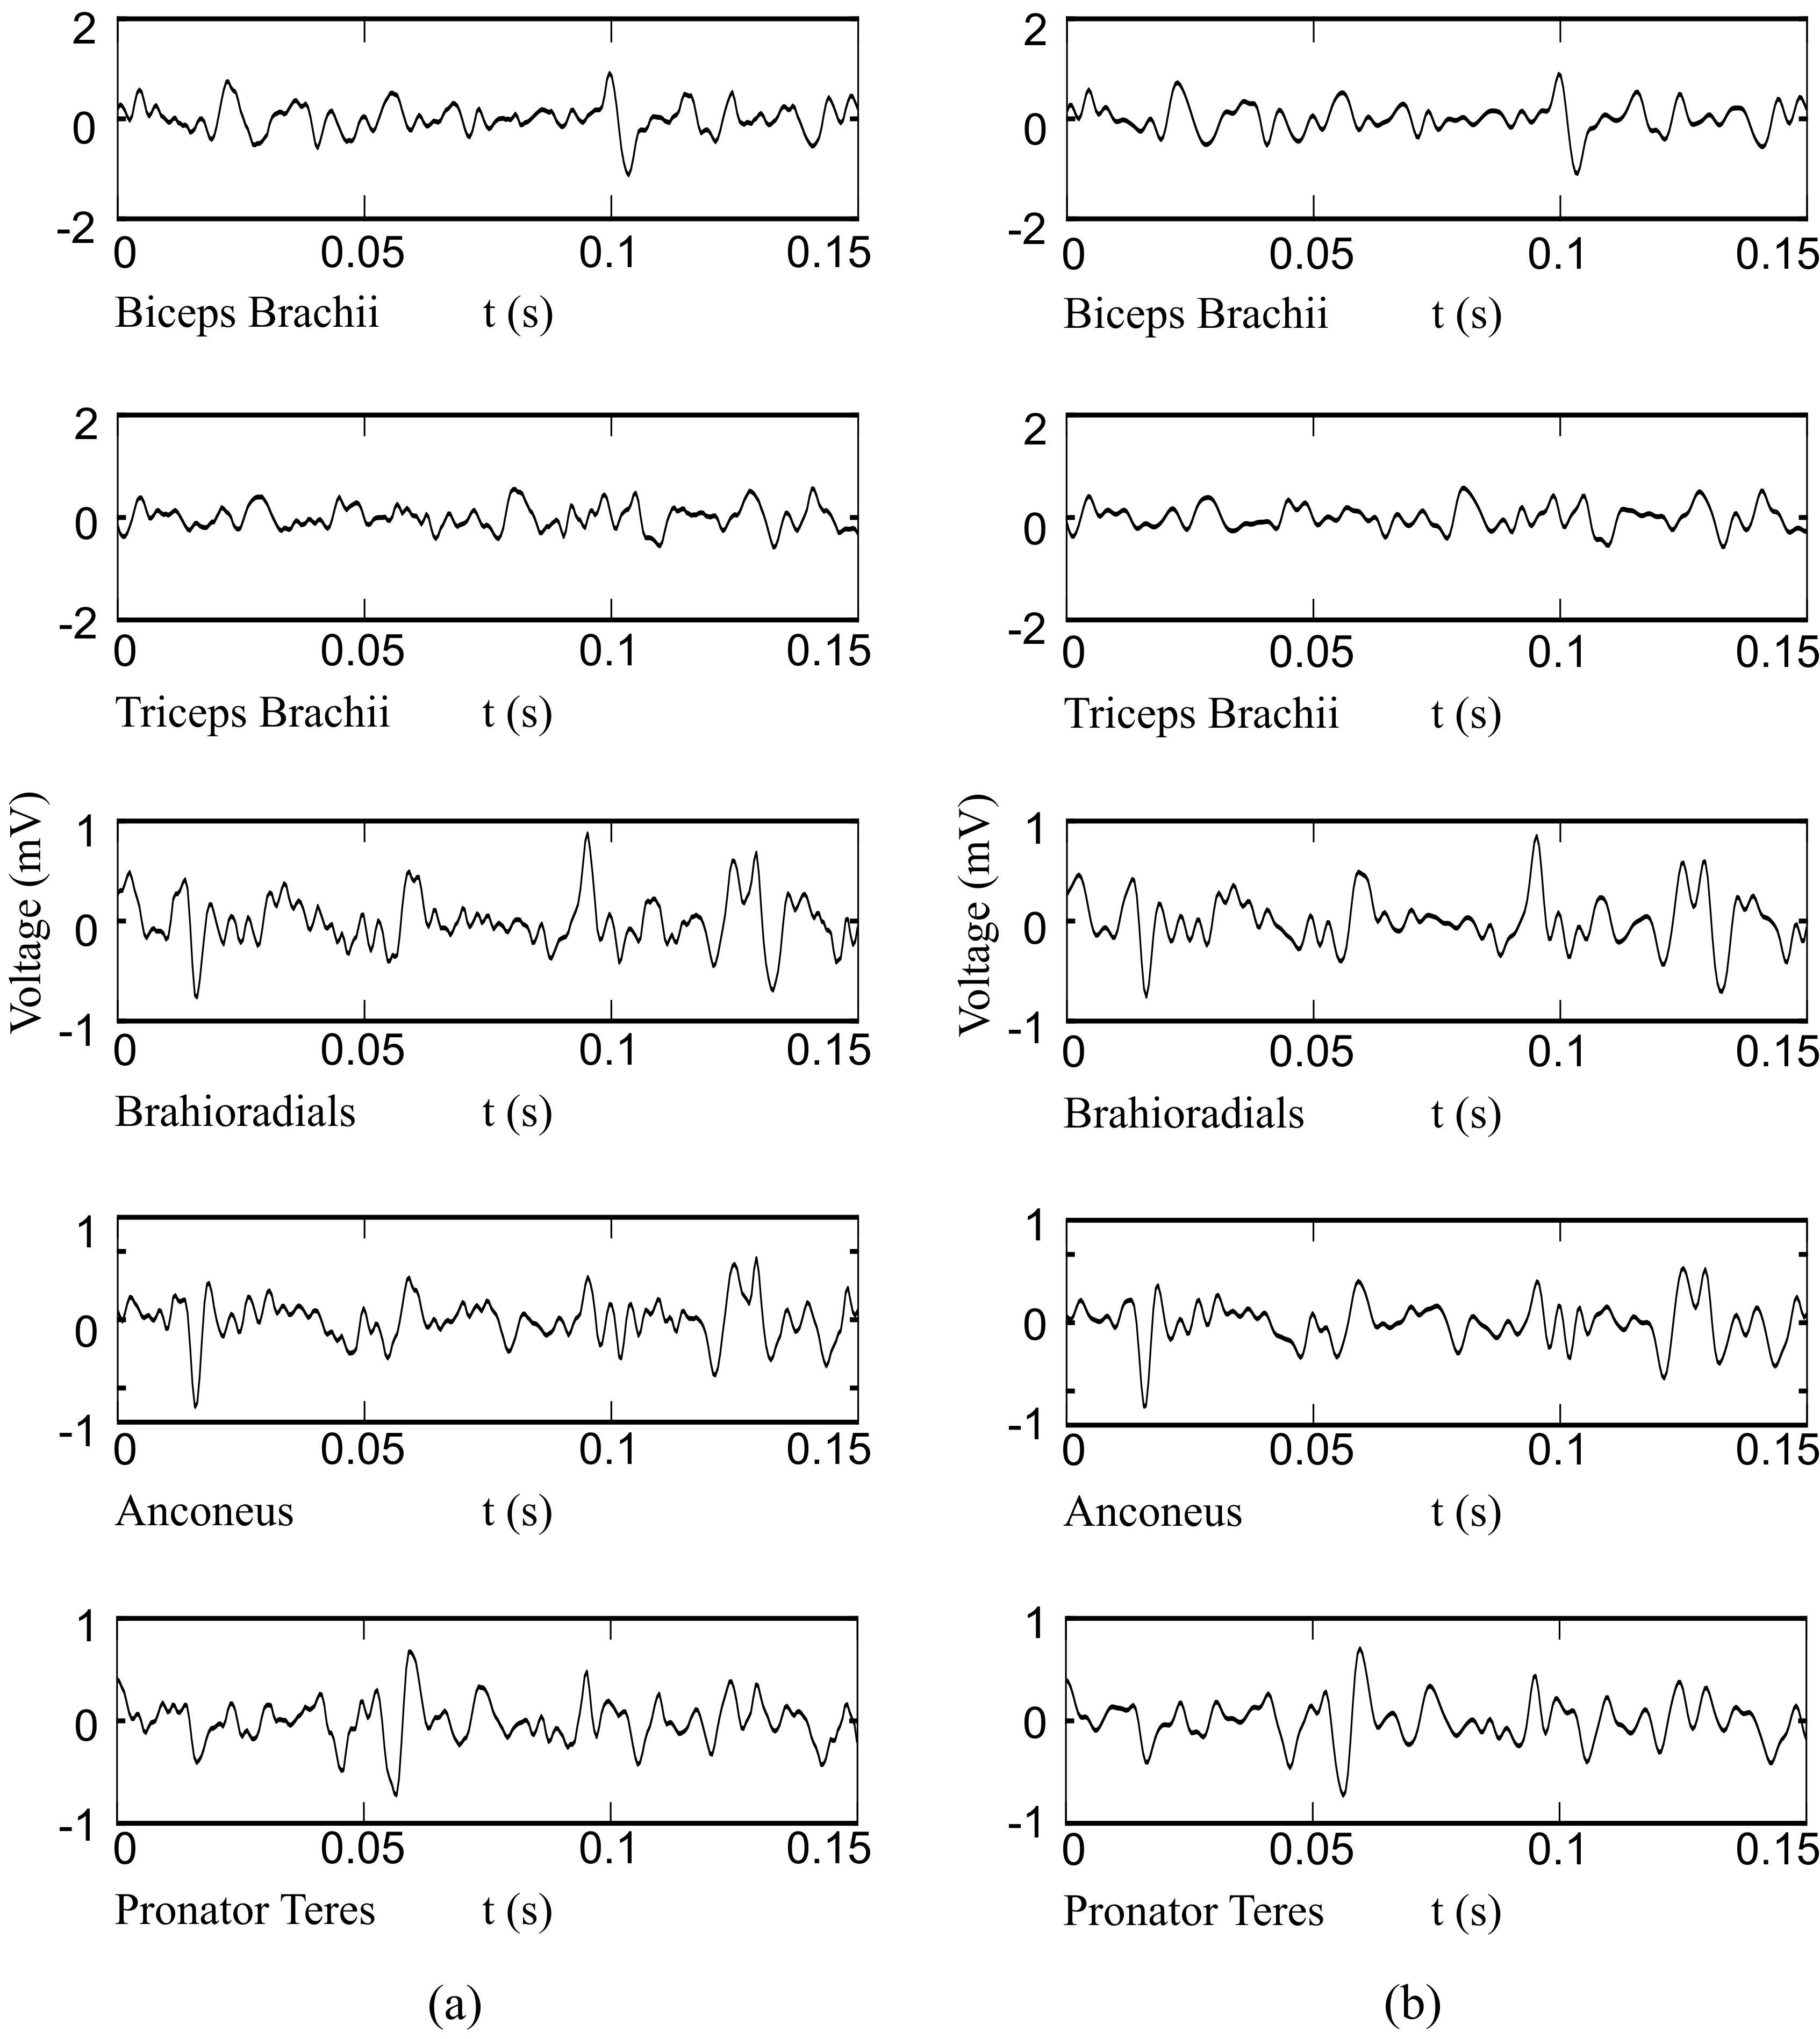
\includegraphics[width=0.99\textwidth]{Images/figure3_B5.png}
\caption{Example of recorded EMG signals from five muscles (biceps brachii, triceps brachi, brachioradialis, anconeus, bracioradialis, and pronator teres) during pronation. Figure shows (a) raw signals and (b) signals filtered using 4\textsuperscript{th} order Butterworth filter with the cut-off frequencies of 15 Hz and 350 Hz.}
\label{fig:3-B5}
\end{figure}   

% body of thesis comes here


\newpage
\thiswillnotshow{\large{Hidden notes} \\ More info at: https://tex.stackexchange.com/questions/9796/how-to-add-todo-notes}
\listoftodos[Notes]

%\chapter{Conclusion}
\label{ch:conclusions}

\section{Summary}

Task identification and movement estimation based on EMG are very popular topics involving different areas in machine learning, and, particularly pattern recognition with many possible applications in assistive and rehabilitation devices. The emergence of high-density EMG (HD-EMG) opened new possibilities for extracting neural information and it has been reported that spatial distribution of HD-EMG intensity is a valuable feature in identification of isometric tasks.

This doctoral thesis investigates further the spatial muscle co-activation patterns of myoelectric activity extracted from the HD-EMG activation maps. HD-EMG was measured on five muscles of forearm and upper arm in monopolar configuration during isometric forearm tasks. Measurements were performed on the group of healthy subjects and on the group of patients with incomplete spinal cord injury.

In the chapters 3 and 4, co-activation patterns of patients with incomplete spinal cord injury were analyzed by the means of pattern-recognition-based identification of task and effort level. Both intensity related features, and spatial features were analyzed. In chapter 3, co-activation patterns were analyzed for each patient individually, whereas in chapter 4, co-activation patterns were analyzed within the group of patients. In spite the great diversity between different patients and their levels and types of injury, similarities between activation patterns were found not only in intensity of myoelectric signal, but also in spatial distribution expressed as center of gravity.

In the chapter 5, novel feature for task identification was proposed. The feature is based on spatial distribution of myoelectric activity recorded by HD-EMG. This new feature was evaluated in identification of task and identification of task and effort level in healthy subjects. The evaluation was performed for each subject individually. 


\section{Main conclusions}

In chapter 3, muscle co-activation patterns were analyzed during four isometric tasks and three effort levels in patients with incomplete spinal cord injury. Intensity-based activation maps were calculated for each muscle and different features were extracted: the average intensity of an HD-EMG map, and the center of gravity of an HD-EMG maps. Using the extracted feature sets, a successful patient-specific task identification method was designed. It is capable to estimate with high accuracy not only the motor task, but also the force. This implies that patients with incomplete spinal cord injury have repeatable co-activation muscular pattern not only in intensity, but also in spatial distribution of intensity over the muscle surface. Moreover, the results lead to the conclusion that spatial distribution of myoelectric activity has significant and discriminative power in classification. Furthermore, adding information on spatial distribution of myoelectric intensity improves not only identification result, but also resilience to fatigue and time effect.

Furthermore, in chapter 4 it was discovered that the repeatable patterns in intensity and spatial distribution besides existing for each patient individually, also exist for the entire group of patient. To demonstrate the existence of distinguishable group-specific patterns in HD-EMG, the identification of different tasks was performed, where classifier was not trained exclusively using the samples of a single patient, but it was trained using the samples of all patients, and tested using the samples of all patients, i.e., group-specific classifier was designed. The existence of the patterns is an interesting result because there should be a high level of variability between patients due to the nature of the injury. Co-activation patterns were found not only between different tasks, but also between different effort levels. Group-specific identification of motion intention in patients with neuromuscular impairment could potentially improve the translation of pattern recognition techniques to clinical practice. Also, the results show that the similarity is greater between patients with similar level of lesion (vertebra at which spinal cord injury occurred). This could also have an interesting implication in translation to the clinical practice because patients with the similar level of injury could be able to use the same assisitive/rehabilitation devices with greater ease. 

Finally, in chapter 5, a novel feature for identification of task and effort level was designed. It is based on the locations of local maxima of the probability density function of HD-EMG activation maps, and is obtained using the mean shift algorithm. The feature was tested on the population of healthy subjects in subject-specific approach, that is, classifier was trained and tested for each subject individually. The feature yields higher identification indices compared to the more classical features, especially in task identification at very low effort level. By analyzing the influence of fatigue and other time-dependent changes (e.g. drying of conductive gel) on identification, novel feature had a very good performance. Since the goal of this study was to analyze different feature sets rather than classification methods, LDA was utilized given that this method is the most commonly used, and is generally recommended for myoelectric interfaces \citep{Hakonen2015}.

Density function from which modes were extracted represents RMS activation maps of the HD-EMG. Although the feature proved to be useful, by calculating RMS value, the information is partially lost. Therefore, the modes, or other statistical measures of the raw HD-EMG, i.e. joint distribution of instantaneous EMG amplitude over the electrode array, could also be a useful feature in identification of motion intention. Furthermore, in the literature, features are often calculated for each channel separately and then selected prior the classification using the, e.g., sequential method \citep{Hargrove2009, Li2017}, selection based on common spatial patterns \citep{Geng2014}, or based on the independent component analysis clustering \citep{Naik2016}. Modes of the HD-EMG density function could be correlated with the channels with discriminative information and could be a useful tool in channel selection.

Finally, the mean shift algorithm can be used for clustering and, since it was shown that the algorithm is most effective in low-dimensional data, image segmentation is one of its most successful applications \citep{Comaniciu2002}. A mode of the density estimate, or in this case, a channel selected by the mean shift algorithm, can be considered as a cluster representative \citep{Hennig2015}, related to the possible image segments, where spatial (pixel locations) and range features (the intensity of the grayscale value) are considered. The advantage of the mean shift is that it can be used for clustering non-convex shapes, albeit, it could segment complex non-convex regions in the activation maps. Since segmentation of the muscle activation map can improve the neuromuscular activity estimation \citep{Vieira2010}, this could be a reason why mean shift features improved the performance of the movement detection system compared with previously published attributes. In addition, the algorithm only requires setting one parameter, bandwidth ($h$) and, unlike in the similar methods, it is not necessary to define the number of expected clusters. This is a big advantage because it does not require a priori knowledge on the number of clusters.

The proposed motor task identification method based on spatial information of myoelectric distribution could contribute to the human-machine interface technology. There are many possible applications for this type of technology, for example computer games, exoskeletons, automatic wheelchairs, rehabilitation robots, prostheses, etc. Nowadays, field of brain-computer interface (BCI) technology is advancing very fast with high investments of leading global corporations. However, non-invasive BCI is still an open problem with low output rate, which can be greatly improved by using EMG-based identification of motor intention. For example, 
Müller-Putz et al. suggest non-invasive hybrid brain-computer interfaces (hybrid BCI) designed as EEG-based system, supplemented with other biological and mechanical signals  \citep{Muller-Putz2015}. Joining EEG and EMG recordings in identification of task intention significantly improves the accuracy of individual EEG or EMG system. EMG usually has higher SNR ratio than EEG and it is widely used in the identification of the motion intention, however, it is prone to malfunction due to fatigue. When fatigue occurs, the supplemented EEG input keeps the identification stable, and increases the robustness of the system. Thus, advances in obtaining methods more robust to fatigue or time effect are very interesting.

Some patients with neuromuscular impairment can weakly activate their muscles, but insufficiently to generate a movement. In these patients, as well as in patients that can generate only weak movements, HD-EMG maps can still be generated and used in identification of motion intention, as demonstrated in this study. This approach could supplement the existing BCI or inertial sensors based prostheses and result in a device with a better performance. For example, \citet{Rohm2013} performed a very interesting study with a single SCI patient. Their neuroprosthesis consisted of a functional electrical stimulation of the forearm and upper arm muscles, and a semiactive elbow orthosis. Using BCI and a shoulder joystick, the patient was able to perform complex hand and elbow tasks from everyday life (e.g. eating an ice cream cone). The reported performance of that study was 70\%, which was remarkable considering the fact that the patient did not have any control over involved muscles. However, performance of similar patients could be increased using hybrid BCI if myoelectric activation exists.

As a limitation of the thesis, it should be noted that the proposed features were tested only in highly controlled conditions of isometric contractions. The experiments during non-isometric contractions should be performed in order to validate the quality of the features in dynamic and more natural movements. Also, the experiment included only four tasks related to the elbow joint. Further analysis should include higher number of more complex tasks related to hand and shoulder. Moreover, all results were obtained during offline analysis. To evaluate practical aspects of the features, the experiment should be repeated using online identification and considering multiple transitions between tasks.


\section{Main contributions}

The original contributions provided by the compendium of publications of this thesis are:

\begin{itemize}
\item The definition of a novel pattern-recognition algorithm for task and force identification. The method was based on combination of intensity and spatial distribution of intensity of myoelectric signal, namely center of gravity. The algorithm was validated in the group of patients with incomplete spinal cord injury in terms of robustness during slow time dependent changes, such as fatigue and drying of conductive gel. The results prove the existence of repeatable co-activation pattern in intensity and spatial distribution for each patient. Furthermore, the pattern exists for different tasks, but also for different effort levels.

\item The co-activation pattern in intensity and its spatial distribution of HD-EMG was identified for the group of patients with spinal cord injury. After the injury there is a coherence between activation patterns of different patients, both task-related and force-related. This coherence can be observed in intensity of HD-EMG, but also in spatial distribution of intensity. Furthermore, greater similarity was found within the group of patients with similar level of injury. This result implies the possibility of building assistive/rehabilitation devices for the group of patients with significantly lower training time.

\item Definition of novel statistical spatial feature derived from the HD-EMG. It was used for the identification of task and effort level in group of healthy subjects. This feature is based on the probability density function of the HD-EMG activation map. 


\end{itemize}

\section{Future Work}
\label{sec:fw}
The work developed in this thesis opens new possibilities in the field of myocontrol in rehabilitation. Some of the most interesting possibilities for future works are the following: 

\begin{description}
\item[Dynamic contractions] \hfill \\ 
	The use of spatial information of myoelectric activity is a novel method which already showed very good results in identification of tasks, both in healthy subjects, and in patients with incomplete spinal cord injury during isometric contractions. Isometric contractions are standard to the field of work, that is, pattern recognition for control of human-machine interfaces, and are a good starting point to test the new feature with respect to more classical features. Recordings during isometric contractions provide measurements with more controlled conditions, i.e., minimized influences related to relative shift of recording electrodes with respect to source of the signal – muscle fiber. Therefore it is a good practice to start using new features in graduate analysis in order to establish reliably and precisely the circumstances in which features are useful. However, further studies are necessary to consider non-isometric contractions, which are closer to real conditions. One of this study was already performed within the scope of the thesis and the results were published:\\
	\small{Rojas-Martínez, M., Alonso, J.F., Jordanić, M., Romero, S., Mañanas, M.A. \textbf{Identificación de tareas isométricas y dinámicas del miembro superior basada en EMG de alta densidad}. \textit{Revista Iberoamericana de Automática e Informática Industrial}, Accepted for publication 2017, JCR 0.390, Q4 in Automation and Control Systems (57/60)}
	
	
%	However, isometric contractions The  the merit of combination of intensity and spatial features for identification of specific group of tasks during isometric contractions, and extends the analysis to identification of dynamic tasks. Research is focused on control strategies of upper-limb in normal subjects. Tasks analyzed in the study are related to hand movement in horizontal plane, which mostly involves movements at shoulder joint. These movements were found important because they are commonly used in rehabilitation robots. Although this research was performed on healthy subjects, methods which are proposed could be used for the design and monitoring of rehabilitation therapies intended for patients with neuromuscular impairment. 
	
%	We are already planning and developing the new framework within which we will record non-isometric upper-limb tasks. In our opinion, real time identification of non-isometric tasks should be the final goal of the project.

\item[Generalized mean shift approach] \hfill \\
	In chapter 5 is explained the motor task identification algorithm that uses the novel spatial feature. This spatial feature is based on the modes of the probability density function of HD-EMG activation maps. Instead, the viability of features based on the  modes of the probability density function of raw HD-EMG signal should be explored. Since the information is partially lost by calculating the RMS value of the signal to obtain the activation maps, using joint distribution of instantaneous EMG amplitude over the electrode array could provide higher identification results.
	
\item[Mean shift approach for channel selection] \hfill \\
	Geng et al. recently proposed a more advanced channel selection method based on common spatial patterns \citep{Geng2014} and Naik et al. propose the channel selection based on the independent component analysis \citep{Naik2016}. Modes of the HD-EMG density function, a novel feature proposed in chapter 5, could be correlated with the channels with discriminative information and could be a useful tool in channel selection.

\item[Real time application] \hfill \\
	The task identification system cannot find application without ability of online processing. Therefore, appropriate recording device along with an optimized processing unit should be built. The device should be able to process the task identification in real time using optimized firmware.

\item[Hybrid brain-computer interface] \hfill \\
	The fusion of EEG and EMG could further improve the results of upper-limb task identification, the study we performed using only HD-EMG recordings both in healthy subjects and iSCI patients. This type of study can have impact on numerous fields of application including brain – computer interfaces (BCI). A goal could be to exploit the fusion of cerebral and neuromuscular information and to quantify the improvements when the innovative technique of HD-EMG is joined with the cerebral activity, what was recently called by the research community a \emph{hybrid BCI} \citep{Muller-Putz2015, Rohm2013}.

\item [Increase of identification fidelity] \hfill \\
	Fidelity of the identification could be increased further by using an adaptive model of classifier that is being constantly updated throughout the exercise in order to compensate for the changes in the myoelectric signal caused by, e.g., fatigue ore sweating. There are several recent publications on this subject \citep{Hahne2015, Vidovic2016, Sensinger2009}.

\item[Spatial distribution of frequency] \hfill \\
	Features extracted from frequency/scale domain proved to be very useful in identification of motor task \citep{Oskoei2007}. In future works, it would be interesting to investigate the spatial distribution of frequency over the muscle in search of the discriminative feature.

\end{description}

\section {Publications derived from the thesis}
\subsection{Journal papers}

\begin{itemize}
\item Jordanić, M., Rojas-Martínez, M., Mañanas, M.A., Alonso, J.F., Marateb, H.R. A Novel Spatial Feature for the Identification of Motor Tasks Using High-Density Electromyography. \textit{Sensors}, 17(7): 1597, 2017, JCR 2.077, Q1 in Instruments and instrumentation (10/58)

\item Rojas-Martínez, M., Alonso, J.F., Jordanić, M., Romero, S., Mañanas, M.A. Identificación de tareas isométricas y dinámicas del miembro superior basada en EMG de alta densidad. \textit{Revista Iberoamericana de Automática e Informática Industrial}, Accepted for publication 2017, JCR 0.390, Q4 in Automation and Control Systems (57/60)

\item Jordanić, M., Rojas-Martínez, M., Mañanas, M.A., Alonso, J.F. Prediction of isometric motor tasks and effort levels based on high-density EMG in patients with incomplete spinal cord injury. \textit{Journal of Neural Engineering}, 13(4): 46002, 2016, JCR 3.465, Q1 in Biomedical Engineering (13/77)

\item Jordanić, M., Rojas-Martínez, M., Mañanas, M.A., Alonso, J.F. Spatial distribution of HD-EMG improves identification of task and force in patients with incomplete spinal cord injury. \textit{Journal of NeuroEngineering and Rehabilitation}, 13(1): 41, 2016, JCR 3.222, Q1 in Rehabilitation (3/65)
\end{itemize}


\subsection{Conference papers}

\begin{itemize}
\item Jordanić, M., Rojas-Martínez, M., Mañanas, M.A. Muscle pattern from HD-EMG applied to identification of movement intention. Summer School on Neurorehabilitation (SSNR 2015), 2015, Valencia, Spain

\item   Jordanić, M., Rojas-Martínez, M., Mañanas, M.A., Alonso, J.F. Use of frequency features of HD-EMG in identification of upper-limb motor task. \textit{Cognitive Area Networks}, 4(1): 19:23, 9. Simposio CEA de Bioingeniería: Interfaces Cerebro-Máquina y Neurotecnologías para la Asistencia y la Rehabilitación, 2017, Badalona, Spain

\item Jordanić, M., Rojas-Martínez, M., Alonso, J.F., Migliorelli, C. Mañanas, M.A. Identificación de Contracciones Isométricas de la Extremidad Superior en Pacientes con Lesión Medular Incompleta mediante Características Espectrales de la Electromiografía de Alta Densidad (HD-EMG). Jornadas de Automática (Bioineniería), 2017, Gijon, Spain

\end{itemize}



%
\newpage
\phantomsection
%\cleardoublepage
\addcontentsline{toc}{chapter}{Bibliography}
\bibliographystyle{abbrvnatnourl}
\narrowlinespacing

%\begin{myquote}
%\begin{flushright}
%\textit{So many books, so little time.} \\Frank Zappa
%\end{flushright}
%\end{myquote}

\bibliography{biblio/thesis}


%\appendix
%% appendices come here



\end{document}